\documentclass[10pt,a4paper]{article}
\usepackage[utf8]{inputenc}
\usepackage{amsmath}		% for some math stuff
\usepackage{amsfonts}
\usepackage{amssymb}
\usepackage{graphicx}		% required to include images to document
\usepackage{trfsigns}		% Laplacetransofrmations Zeichen
\usepackage{float}			% gives the option [H] for figures to make them appear according to source code. Otherwise figures may shift to a different page wich is confusing without references

\usepackage[hyperref]{ntheorem} % das [hyperref] wird benötigt um mit dem Paket hyperref kompatibel zu sein
\usepackage{mdframed}		% package to make frames for exaples, definitions and theorems
							% http://www.ctan.org/tex-archive/macros/latex/contrib/mdframed/

\usepackage[hidelinks]{hyperref}		% use table of contents liek links

\global\mdfdefinestyle{satz}{linecolor=red,linewidth=2pt,skipabove=10pt,skipbelow=5pt}
% \mdtheorem[style=satz]{satz}{Satz} % indexing didn't work with this, mdframed doku confirms this
\newmdtheoremenv[style=satz]{satz}{Satz}

\global\mdfdefinestyle{defi}{linecolor=green,linewidth=2pt,skipabove=10pt,skipbelow=5pt}
% \mdtheorem[style=defi]{defi}{Definition} % indexing didn't work with this, mdframed doku confirms this
\newmdtheoremenv[style=defi]{defi}{Definition}

\global\mdfdefinestyle{bsp}{linecolor=blue,linewidth=2pt, skipabove=10pt,skipbelow=5pt}
% \mdtheorem[style=bsp]{bsp}{Beispiel} % indexing didn't work with this, mdframed doku confirms this
\newmdtheoremenv[style=bsp]{bsp}{Beispiel}


\author{Benedict Simlinger, published by \url{http://latex4ei.de/}}
\title{Mitschrift von "Höhere Mathematik 4", Sommer 2013, Prof. Ulbrich}

\renewcommand*\contentsname{Inhaltsverzeichnis}

% für indexing of examples, satz and definition
% http://tex.stackexchange.com/questions/74857/toc-like-list-of-definitions-using-theorem-environments
% http://tex.stackexchange.com/questions/3899/how-to-create-an-index-for-custom-environments
% http://texblog.org/2008/07/13/define-your-own-list-of/


\begin{document}

\maketitle
\tableofcontents
\newpage



\section{Gewöhnliche DGL}


\subsection{nichtlineare DGL erster Ordnung}

Eine nichtlineare DGL hat die Form 

\begin{eqnarray}
y'(x)&=& f(x, y(x)) \\
&&x \in I \in \mathbb{R} \nonumber \\
&&f(x,y) \in I \times \mathbb{R} \rightarrow \mathbb{R} \nonumber
\end{eqnarray}

 und gesucht wird ein $y(x), I \rightarrow \mathbb{R}$ welches diese Gelichung erfüllt, wobei $f(x,y)$ mindestens stetig sein muss.

Ein Anfangswertproblem (AWP) liegt vor, wenn eine DGL und deren Anfangswerte $y(x_0)=y_0$ gegeben ist. Bei solchen AWPs stellt sich die Frage nach
\begin{itemize}
\item Existenz
\item Eindeutigkeit
\item Lösungsweg
\end{itemize}

\subsubsection{DGL mit getrennten Variablen}
DGLs mit trennbaren Variablen haben die Form 
\begin{equation}
y'(x)=f(x) \cdot g(y(x))
\end{equation}

Mit einer formalen Taschenspielerei trennt man die Variablen


\begin{eqnarray*}
					y(x)'					&=&f(x) \cdot g(y(x)) \\
\Leftrightarrow		\frac{dy}{dx}			&=&f(x) \cdot g(y(x)) \\
\stackrel{g(y(x)) \not= 0}{\Leftrightarrow	}	\frac{1}{g(y(x))}dy	&=&f(x)dx
\end{eqnarray*}


Wenn man nun statt $g(y(x))$ schreibt $g(y)$ sieht man, dass alles was mit $y$ zu tun hat, links steht, und alles was mit $x$ zu tun hat, rechts steht. Weiter geht es mit 

\begin{eqnarray*}
\underbrace{\int \frac{1}{g(y(x))} dy}_{G(y)} &=& \underbrace{\int f(x)dx}_{F(x)} + c \\
G(y)-F(x) &=& c
\end{eqnarray*}

Die Integrale ausrechnen und eine Umformung nach $y$ führen dann zur Lösung, wobei die Konstante $c$ die Integrationskonstante ist, die sich aus den Anfangswerten berechnet, wie wir später sehen werden.

Für den Fall $g(y_0)=0$ gilt

\begin{equation}
g(y_0)=0 \rightarrow y = y_0
\end{equation}

Sind die Anfangswerte gegeben, so gilt 

\begin{eqnarray*}
G(y)=\int_{y_0}^{y} \frac{1}{g(\eta)} d\eta \\
F(x)=\int_{x_0}^{x}f(\xi) d\xi
\end{eqnarray*}


als die Lösung des Problems. Beachte, dass hier keine Integrationskonstanten mehr vorkommen!



\begin{satz}[Existenz- und Eindeutigkeitssatz für trennbare DGL]

\begin{equation*}
\begin{array}{rl} 
$Sei$ & f ~ $in$ I_x = \{x|a \leq x \leq b\} $stetig, $ x_0 \in I_x$,$ \\
$und$ & g~$in $I_y =  \{y|a \leq y \leq b\} $stetig, $ y_0 \in I_y 
\end{array}
\end{equation*}

und es gilt

\begin{equation*}
\begin{array}{rl} 
$entweder$ & g(y_0) \not= 0 \\
$oder$ & g(y_0)=0$ mit $\left| g(y) \right| \leq L\left| y-y_0\right|
\end{array}
\end{equation*}

dann besitzt das AWP 

\begin{equation*}
y'=f(x) \cdot g(y)
\end{equation*} in der Umgebung von $x_0$ eine eindeutige Lösung.
\end{satz}



\begin{bsp}[$y'=xy$]
\begin{equation*}y'=\underbrace{x}_{f(x)} \underbrace{y}_{g(y)}\end{equation*}
Für $y=0$ 
\begin{equation*}g(y)=g(0)=0 \Rightarrow y'=0 \Rightarrow y(t)=const. \end{equation*}

\noindent Für $y \not= 0 $

\begin{eqnarray*}
G(y)=\int \frac{1}{g(y)} = \int \frac{1}{y} dy &=& F(x) = \int x dx +c \\
\Leftrightarrow ln \left| y \right| &=& \frac{x^{2}}{2} +c_1 \\
\Leftrightarrow \left| y \right| &=& e^{x^{2}/2 + c_1} \\
\Leftrightarrow \left| y \right| &=& \underbrace{e^{x^{2}/2}}_{>0} \cdot \underbrace{e^{c_1}}_{ > 0} \\
\Rightarrow y &=& \underbrace{\pm c_2}_{\not= 0} \cdot e^{x^{2}/2}, ~ c_2 \in \mathbb{R}
\end{eqnarray*}
\end{bsp}

\begin{bsp}[$y'=2xy^{2}+2x$]

Gegeben ist $y(0)=y_0=1, x_0=0$ und $y'=\underbrace{2x}_{f(x)}\underbrace{(y^{2}+1)}_{g(y)}$

Da es von $g(y)$ keine Nullstellen gbt, gibt es auch keine spezielle konstante Lösung.

\begin{eqnarray*}
G(y)= \int^{y}_{y_0} \frac{1}{z^{2}+1}dz &=& F(x) = \int^{x}_{x_0} 2s ds \\
\arctan(y)-\underbrace{\arctan(1)}_\frac{\pi}{2} &=& x^{2} \\
\arctan (y) - \frac{\pi}{4} &=& x^{2} \\
y &=& \tan(x^{2}+\frac{\pi}{4})
\end{eqnarray*}


\end{bsp}

\begin{bsp}[$y'=y^{2}$]

Für $y(0)=y_0 = 0$ ergibt sich die konstante Lösung $y=0$

\noindent Für $y(0)=y_0 \not= 0$ gilt mit $f(x)=1, g(y)=y^{2},x_0=0$

\begin{eqnarray*}
\underbrace{\int^{y}_{y_0} \frac{1}{z^{2}}dz}_{G(y)} &=& \underbrace{\int^{x}_{0}1ds}_{F(x)} \\
- \frac{1}{y} + \frac{1}{y_0} &=&x \\
y &=& \frac{y_0}{1-y_0x}, ~ x \not= \frac{1}{y_0}
\end{eqnarray*}


\end{bsp}

\subsubsection{Existenz- und Eindeutigkeitssätze für AWP}


\begin{bsp}[$y'=1+y^{2}$]

\begin{eqnarray*}
\int_{0}^{y}\frac{1}{1+z^{2}} dz &=& \int_{0}^{x}1 ds \\
\arctan(y)&=&x \\
y(x)&=& \tan(x)
\end{eqnarray*}

Allerdings gilt diese Lösung nur solange $x \in (-\frac{\pi}{2},\frac{\pi}{2})$
\end{bsp}

Das obige Beispiel zeigt, dass Lösungen auf gewissen Umgebungen, wie in diesem Fall $-\frac{\pi}{2}\leq x \leq \frac{\pi}{2}$ begrenzt werden müssen.

\begin{bsp}[$y'=\sqrt{\left| y\right|}$]
$y'=\sqrt{\left| y\right|}=y^{\frac{1}{2}}, ~ y(x_0)=0$ 

Für $y(x)=0$ ist die konstante Lösung sofort erkennbar.

Für $y>0$

\begin{eqnarray*}
\int y^{-\frac{1}{2}} dy &=& \int 1 dx \\
2y^{\frac{1}{2}} &=& x +c \\
y(x) &=& \left( \frac{x+c}{2}\right)^{2} \\
\stackrel{y(x_0)=0}{\Rightarrow} y(x) &=&  \left( \frac{x-x_0}{2}\right)^{2} = \frac{1}{4}(x-x_0)^{2}\\
\end{eqnarray*}

Für $y<0$ ergibt sich analog $-\frac{1}{4}(x-x_0)^{2}$

Durch jeden Punkt $(x_0,0)$ verlaufen also mehrere Lösungen

\begin{itemize}
\item $y(x)=0$
\item $\frac{1}{4}(x-x_0)^{2}$ für $y >0$
\item $ -\frac{1}{4}(x-x_0)^{2}$ für $y<0$
\end{itemize} 

\noindent Wir sehen, es gibt in keinem Punkt der $x$-Achse eine eindeutige Lösung, da sich die obigen Varianten beliebig kombinieren lassen. Da die Wurzelfunktion nicht lipschitzstetig ist (d.h. die Steigung der Funktion ist nicht durch eine Konstante beschränkt) kommt es in diesem Beispiel zur Nicht-Eindeutigkeit der Lösung.

\end{bsp}


\begin{defi}[Lipstetigkeit und Lokale Lipstetigkeit]
Sei $G \subseteq \mathbb{R}^{2}$ ein Gebiet und $f: G \rightarrow \mathbb{R}$
\begin{itemize}
\item $f$ ist lipschitzstetig bezüglich $y$ wenn es eine Konstante $L \geq 0$ gibt, so dass $\left| f(x,y_1)-f(x,y_2) \right| \leq L \left| y_1 - y_2 \right| \forall (x,y_1), (x,y_2) \in G$
\item $f$ ist lokal lipstetig bezüglich y, wenn es in jedem Punkt von G eine Umgebung $U$ gibt, so dass $f$ lokal lipschitzstetig bezüglich y in $G \cap U$ ist
\end{itemize}
\end{defi}

\begin{satz}[Aus Stetigkeit folgt lokale Lipstetigkeit]

Ist $\partial_y f$ stetig auf G, dann ist f lokal lipstetig bezüglich y auf G. Dies folgt aus $f(x,y_2)-f(x,y_1)=\int^{y_2}_{y_1} \partial_y f(x,y)dy < L \left| y_2-y_1\right|$ falls $\left| \partial_y f(x,y) \right| \leq L \forall y \in [y_1,y_2]$
\end{satz}
\begin{bsp}[$f(x,y)=\left| y \right|$]
$f$ ist global lipstetig bezüglich y mit $L=1$
\end{bsp}

\begin{bsp}[$f(x,y)=x+x^{2}y^{2}$]

\begin{eqnarray*}
|f(x,y_1) - f(x,y_2)| &=& \\
x^{2}| y_1^{2} - y_2^{2} | &=& \\
x^{2}| y_1+y_2| \cdot |y_1+y_2| & \leq & L | y_1-y_2|
\end{eqnarray*}
$$\forall (x,y_i) ~mit~  x^{2} \left|y_1+y_2\right| \leq L$$

Dieses Beispiel ist nur lokal lipstetig, da für 

\begin{equation*}
\left. \begin{matrix}
| x| \rightarrow \infty \\
oder \\
| y_i| \rightarrow \infty
\end{matrix}
\right\rbrace \Rightarrow L \rightarrow \infty
\end{equation*}

Übrigens hätten wir mit dem vorherigen Kriterium die Stetigkeit von 

\begin{equation*}
f(x,y) = 2x^{2}y
\end{equation*} 

gesehen und damit die lokale Lipstetigkeit gesehen.

\end{bsp}

\begin{bsp}[$f(x,y)= \sqrt{\left| y\right|}$]

Wir sehen uns die Funktion in der Umgebung von $y=0$ an
\begin{equation*}
y_1=0
\end{equation*}
und prüfen auf Lipstetigkeit

\begin{eqnarray*}
|f(x,y_1)-f(x,y_2)| & \leq & L | y_2-y_1 | \\
\left| \frac{f(x,y_1)-f(x,y_2)}{ y_2-y_1 } \right| & \leq & L
\end{eqnarray*}

Anmerkung: Man beachte, dass wir mit der obigen Formel prüfen, ob die Steigung einer Funktion durch einen Wert $L$ begrenzt wird.

\begin{eqnarray*}
\left| \frac{\overbrace{f(x,y_1)}^{0}-f(x,y_2)}{ y_2-\underbrace{y_1}_0 } \right| & \leq & L \\
\frac{\sqrt{\left| y_2\right|}}{ | y_2|} & \leq & L\\
\frac{1}{\sqrt{\left| y_2\right|}} &\leq & L\\
y_2 \rightarrow 0 &\Rightarrow & L \rightarrow \infty
\end{eqnarray*}
Es gibt keine lokale Lipstetigkeit, denn die Steigung der Wurzelfunktion am Punkt Null ist unendlich.
\end{bsp}

Anmerkung:
Aus lokaler lipstetigkeit folgen Aussagen über Existenz und Eindeutigkeit.

\begin{satz}[Eindeutigkeit von Lösungen]
Sei $f$ auf dem Gebiet $G \subseteq \mathbb{R}^{2}$ stetig und erfüllt lokale Lipstetigkeit bezüglich y auf G. Dann gibt es zu jedem $(x_0,y_0) \in G$ für das AWP 
\begin{equation*}
y'=f(x,y),~ y(x_0)=y_0
\end{equation*}
eine eindeutige Lösungskruve $y(x)$ die beidseitige dem Rand von G beliebig nahe kommt.
\end{satz}

Der Beweis wird über die Picarditeration (eine Form der Fixpunktiteration) geführt. Dazu formt man das AWP um 
\begin{eqnarray*}
y'(x)&=&f(x,y(x)) \\
\int^{x}_{x_0} y'(s) ds &=& \int^{x}_{x_0} f(s,y(s)) ds \\
y(x)-y(x_0) &=& \int^{x}_{x_0} f(s,y(s)) ds \\
y(x) &=&\underbrace{y_0}_{y(x_0)} +  \int^{x}_{x_0} f(s,y(s)) ds
\end{eqnarray*}


Nun führt man die Picarditeration nach folgendem Muster durch
:
Wähle $y_0$, bestimme $F(y_0)=y_1, F(y_1)=y_2, u.s.w.$

\begin{eqnarray*}
y_0(x)&=&y_0 \\ 
y_k(x)&=&y_0 + \int^{x}_{x_0}f(s,y_{k-1}(s))ds , ~ k=1,2,3,\ldots
\end{eqnarray*}


\begin{bsp}[$y'=2xy$ Lösung über Separation der Variablen]
$$y'=2xy, ~ y(\underbrace{0}_{x_0})=\underbrace{1}_{y_0}$$  
$$y(x)=e^{x^{2}}$$
\end{bsp}

\begin{bsp}[$y'=2xy$, Lösung über Picarditeration]

\begin{eqnarray*}
y_0(x)&=&1 \\
y_1(x)&=&1 + \int^{x}_{0} 2s \cdot 1 ds = 1+x^{2} \\
y_2(x)&=&1 + \int^{x}_{0} 2s \cdot \left(1+s^{2}\right) ds = 1+x^{2}+\frac{1}{2}x^{4} \\
y_3(x)&=&1 + \int^{x}_{0} 2s \cdot \left(1+s^{2}+\frac{1}{2}s^{4}\right) ds = 1+x^{2}+\frac{1}{2}x^{4} + \frac{1}{6}x^{6} \\
y_4(x)&=&1 + \int^{x}_{0} 2s \cdot \left(1+x^{2}+\frac{1}{2}x^{4} + \frac{1}{6}x^{6}\right) ds\\
&=& 1+ x^{2} + \frac{1}{2}x^{4} + \frac{1}{6}x^{6}+\frac{1}{24}x^{8}\\
 & \vdots & \\
y_n(x)&=&\sum^{n}_{k=0} \frac{x^{2k}}{k!} \xrightarrow{n \rightarrow \infty} e^{x^{2}}
\end{eqnarray*}

\end{bsp}

\noindent Das Ergebnis ist offensichtlich das Gleiche. Der Vollständigkeit halber müssten man noch die Aussage per vollsändiger Induktion überprüfen. Nun stellt sich noch die Frage: Wie stark hängt die Lösung von den Anfagnswerten ab?

\begin{satz}[stetige Abhängigkeit von Anfangswerten]
Erfüllt die stetige Funktion $f(x,y)$ auf den Gebiet $G \subseteq \mathbb{R}$ die Lipschitzbedingung bezüglich $y$, dann gilt für je zwei in G verlaufende Lösungen $y_1(x), y_2(x)$ von $y'=f(x,y)$ die Abschätzung

\begin{equation*}
\underbrace{|y_1(x)-y_2(x)|}_{\Delta_x} \leq \underbrace{|y_1(x_0)-y_2(x_0)|}_{\Delta_{x_0}}e^{L|x-x_0|}
\end{equation*}
\end{satz}

Anmerkung:
$L$ ist die Lipschitzkonstante (die immer auf den "worst case" ausgelegt wird)
Analog gilt dies auch für den mehrdimensionalen Fall.

\begin{figure}[H]
\centering
\includegraphics[width=\textwidth]{images/dependence_on_startvalues.pdf}
\caption{Veranschaulichung der Abhängikeit von DGLen von Anfangswerten}
\end{figure}


\subsection{DGLn n-ter Ordnung}

Wir betrachten die DGL n-ter Ordnung 

\begin{equation}
y^{(n)}(x)=f(x,y(x),y'(x),...,y^{(n-1)}(x)) , ~ n \geq 1
\end{equation}

\subsubsection{Rückführung auf ein System erster Ordnung}

Die DGL n-ter Ordnung kann mit Hilfe von Hilfsfunktion in ein System erster Ordnung überführt werden.

\begin{eqnarray*}
z_1(x)&=&y(x) \\
z_2(x)&=&y'(x) \\
& \vdots & \\
z_n(x)&=&y^{(n-1)}(x)
\end{eqnarray*}


Klarerweise ergibt sich daraus auch

\begin{eqnarray*}
z_1(x)'		&=		&z_2(x) \\
z_2(x)'		&=		&z_3(x) \\
			&\vdots	& \\
z_{n-1}(x)'	&=		&z_n(x) \\
z_n'(x)		&=		& f(x,\underbrace{ z_y(x)}_{y(x)}, \underbrace{z_2(x)}_{y'(x)},..., \underbrace{z_n(x)}_{y^{(n-1)}(x)})
\end{eqnarray*}

Es gilt also

\begin{equation}
\begin{pmatrix}
z_1 \\ z_2 \\ z_3 \\ \vdots \\ z_n
\end{pmatrix}' = 
\begin{pmatrix}
z_2 \\z_3 \\z_4\\ \vdots \\ f(x, z_1(x),\ldots, z_n(x))
\end{pmatrix}
%=
%\begin{pmatrix}
%y' \\ y'' \\ y^{(3)} \\ \vdots \\ y^{(n)}
%\end{pmatrix}=
%\begin{pmatrix}
%y \\ y' \\ y'' \\ \vdots \\ y^{(n-1)}
%\end{pmatrix}'
\end{equation}

Löst $z$ die DGL, dann gilt diese Lösung wegen

\begin{equation}
\begin{pmatrix}
z_1 \\ z_2 \\ z_3 \\ \vdots \\ z_n
\end{pmatrix}'=
\begin{pmatrix}
y \\ y' \\ y'' \\ \vdots \\ y^{(n-1)}
\end{pmatrix}'=
\begin{pmatrix}
y' \\ y'' \\ y^{(3)} \\ \vdots \\ y^{(n)}
\end{pmatrix}=
\begin{pmatrix}
y' \\ y'' \\ y^{(3)} \\ \vdots \\ f(x,y(x),y'(x),...,y^{(n-1)}(x))
\end{pmatrix}
\end{equation}

auch für $y(x)$!

Der springende Punkt ist, die verschiedenen Ableitungen von $y$ als "unabhängige" Gleichungen in $z$ wahrzunehmen, auch wenn der Zusammenhang der verschiedenen $z_i$ über die Ableitungen erhalten bleibt. Durch diese Überfürhungs sieht man auch sehr schön, dass man für DGLn $n$-ter Ordnung auch $n$ Anfangswerte braucht, wodurch sich ein AWP nun wie folgt schreibt

\begin{defi}[AWP $n$-ter Ordnung]
\begin{equation}
y^{(n)}(x)=f(x,y(x),y'(x),...,y^{(n-1)}(x))
\end{equation}

\begin{eqnarray*}
y(x_0)&=&y_0\\
y'(x_0)&=&y_1\\
&\vdots&\\
y^{(n-1)}(x_0)&=&y_{n-1}
\end{eqnarray*}

\end{defi}

\subsubsection{Lineare DGLn $n$-ter Ordnung mit konstanten Koeffizienten}

Wir betrachten mit diesem Wissen nun wieder die lineare DGL n-ter Ordnung (diesmal in Abhängigkeit von $t$ wegen des engen Zusammenhangs mit LTIs)
\begin{eqnarray}
L[y] = a_n y^{(n)}+ a_{n-1} y^{(n-1)} + ... + a_1 y' + a_0 y=b(t) \\
 ~a_n \not= 0,~ a_k \in \mathbb{R}
\end{eqnarray}

Wir bringen das System in die Form

\begin{equation}
y^{(n)} = -\frac{a_{n-1}}{a_n} y^{(n-1)} - \ldots -\frac{a_1}{a_n} y' -\frac{a_0}{a_n} y + \frac{b}{a_n}
\end{equation}


Mit der Überführung in das Begelitsystem
\begin{equation}
\begin{pmatrix}
z_1(x) \\
z_2(x)\\
\vdots\\
z_n(x)
\end{pmatrix} = 
\begin{pmatrix}
y(x) \\
y'(x) \\
\vdots\\
y^{(n-1)}(x)
\end{pmatrix}
\end{equation}



\begin{equation}
\begin{pmatrix} z_1 \\ z_2 \\ \vdots \\ \vdots \\ z_{n-1} \\ z_n \end{pmatrix}' = 
\begin{pmatrix}
0  &1 	& 0		& \ldots	& 0 & 0\\
0  &0  	& 1 	&			& 0 & 0\\
\vdots  &\vdots	& 0 	& \ddots & \vdots &\vdots \\
\vdots  &\vdots  &\vdots  &\ddots &1 & 0\\
0  &0	& 0& 	& 0 & 1\\
-\frac{a_0}{a_n}  &-\frac{a_1}{a_n}		&   -\frac{a_2}{a_n}		& \ldots & -\frac{a_{n-2}}{a_n}& -\frac{a_{n-1}}{a_n}
\end{pmatrix}
\begin{pmatrix} z_1 \\ z_2 \\\vdots \\ \vdots \\ z_{n-1} \\ z_n \end{pmatrix} + 
\begin{pmatrix} 0 \\ 0 \\ \vdots \\  \vdots \\ 0 \\ \frac{b}{a_n} \end{pmatrix}
\end{equation}

Das Begleitsystem hat also die Form $z' = Az + b$. Man kann nun die Lösungstheorie von lin. DGL-Systeme erster Ordnung anwenden.

Es gilt wie bereits festgestellt: Ist $y$ die Lösung der DGL $\Leftrightarrow$ z ist Lösung des Begleitsystems

\subsection{Die homogene DGL n-ter Ordnung}

Homogene DGLn n-ter Ordnung lassen sich wie folgt darstellen
\begin{equation}
L[y]=a_n y^{(n)}+ a_{n-1} y^{(n-1)} + ... + a_1 y' + a_0 y = 0
\end{equation}


Das charakteristische Polynom einer solchen DGL lautet

\begin{equation}
P(\lambda)= a_n \lambda^{n}+ a_{n-1} \lambda^{n-1} + ... + a_1 \lambda + a_0
\end{equation}

Die Nullstellen $\lambda_1,..., \lambda_n \in \mathbb{C}$ des char. Polynom mit den jeweiligen  Vielfachheiten $k_1,...,k_r$ (wobei $ k_1+...+k_r = n$) stellen gleichzeitig die Eingenwerte der allgemeine Basislösung dar.

Zum Eigenwert $\lambda_j$ mit Viefachheit $k_j$ bilden sich $k_j$ Basislösungen

\begin{equation}
e^{\lambda_j t}, t e^{\lambda_j t}, ... , t^{k_j -1} e^{\lambda_j t}
\end{equation}

Dies für $j=1,... r$ liefert ein komplettes System von Basislösungen für die homogene Gleichung.
 
Falls eine reelle Lösungsbasis gesucht ist gilt:

\begin{equation}
\lambda_j \in \mathbb{C}  \backslash \mathbb{R} \Rightarrow \exists i \not= j: \lambda_i = \overline{\lambda_j}
\end{equation}

Was bedeutet diese Formel? Sie besagt, dass sich koplexe Eigenwerte bilden können, die aber immer in komplex-konjugierten Paaren auftreten, also zum Beispiel  $\lambda_j=\alpha_j +i \beta_j$ und $\lambda_i = \overline{\lambda_j}=\alpha_j -i \beta_j$

%\begin{eqnarray*}
%e^{\lambda_j t} + e^{\lambda_i t}=e^{\lambda_j t} + e^{\overline{\lambda_j} t}
%&=& e^{(\alpha_j +i \beta_j) t} + e^{(\alpha_j - i \beta_j) t} \\
%&=&e^{\alpha_j t}e^{i \beta_j t} + e^{\alpha_jt}e^{-i \beta_j t} \\
%&=&e^{\alpha_j t}(e^{i \beta_j t}+e^{-i \beta_j t}) \\
%% &\stackrel{e^{i \varphi} = \cos(\varphi) + i \sin(\varphi)}{=}&
%&=& e^{\alpha_j t}(\cos(\beta_j t) + i \sin(\beta_j t)) +\\
%& & e^{\alpha_j t}(\cos(- \beta_j t) + i \sin(-\beta_j t))
%\end{eqnarray*}

Wegen

\begin{eqnarray*}
\mathrm{Re}[e^{\lambda_j t}] &=& e^{\alpha_j t} \cos(\beta_j t) \\
\mathrm{Im}[e^{\lambda_j t}] &=& e^{\alpha_j t} \sin(\beta_j t) \\
\lambda_j &=& \alpha_j +i \beta_j \\
0 &\leq&  l \leq k_j -1
\end{eqnarray*}

sind die Lösungsbasen

\begin{eqnarray*}
e^{\alpha_j t} \cos(\beta_j t), ~ t e^{\alpha_j t} \cos(\beta_j t), ~t^{2}e^{\alpha_j t} \cos(\beta_j t), \ldots t^{k_j-1}e^{\alpha_j t} \cos(\beta_j t)  \\
e^{\alpha_j t} \sin(\beta_j t), ~ t e^{\alpha_j t} \sin(\beta_j t), ~t^{2}e^{\alpha_j t} \sin(\beta_j t), \ldots t^{k_j-1}e^{\alpha_j t} \sin(\beta_j t)  
\end{eqnarray*}


%Herleitung der Formeln efolgt über das Fundamentalsystem $Z(t)$ des Begleitsystem $z' = Az$
%
%$Z(t)=(z_1(t),...., z_n(t)) = \begin{pmatrix}
%y_1(t) && \ldots && y_n(t)\\
%y_1'(t) && \ldots && y_n'(t) \\
%\vdots && \vdots && \vdots \\
%y_1^{(n-1)}(t) && \ldots && y_n^{(n-1)}(t)
%
%\end{pmatrix}$
%
%Die Eigenwerte von A stimmen mit den Nullstellen des char. Polynoms überein!
%
%$det(A-\lambda I) = $ Entwicklung nach letzter Zeile $= \frac{(-1)^n}{a_n}P(\lambda)$

\begin{bsp}[$ L(y) =y''-2y'+y $]
\begin{equation*}
\Rightarrow a_2=1, a_1=-2, a_0=1
\end{equation*}
Das charakteristische Polynom lautet also
\begin{eqnarray*}
P(s)&=&s^{2}-2s+1\\
&=&(s-1)^{2}
\end{eqnarray*}
Daraus folgt 
\begin{equation}
 \lambda_{1}=1 , ~ k_1=2
\end{equation}

System von Basislösungen 
\begin{eqnarray*}
e^{\lambda_1 t}, t e^{\lambda_1 t} \rightarrow e^{ t}, t e^{ t}
\end{eqnarray*}
\end{bsp}


% ============================================================ Vorlesung 23.4

\subsubsection*{Wiederholung Homogene DGL n-ter Ordung $L[y]=0$}

\begin{equation}
L[y] = a_n y^{(n)}+ a_{n-1} y^{(n-1)} + ... + a_1 y' + a_0 y
\end{equation}

Es folgt eine Zusammenfassung des zuvor besprochenen Lösungsweges:

\begin{enumerate}
\item Bestimme char. Polynom P und dessen Nullestellen $\lambda_1, ..., \lambda_r$ mit Vielfachkeiten  $k_1 , ..., k_r $
\item Basislösungen zu $\lambda_j$ : $e^{\lambda_j t},t e^{\lambda_j t}, ..., t^{k_j-1} e^{\lambda_j t} $ Dies liefert ein System von n Basislösungen
\item ggf. reell machen \begin{enumerate}
\item$\lambda_j \in \mathbb{R} \Rightarrow e^{\lambda_j t},t e^{\lambda_j t}, ..., t^{k_j-1} e^{\lambda_j t} $ sind bereits reell
\item $\lambda_j, \lambda_i = \overline{\lambda_j}$ konjugiert-komplexe Nullstellenpaare ($\lambda_j \notin \mathbb{R}$) mit $$\lambda_j= \alpha_j + i\beta_j $$ zu $$e^{\alpha_j t}(cos(\beta_j t)+\sin(\beta_j t))$$ $$ t e^{\alpha_j t}(cos(\beta_j t)+\sin(\beta_j t)), ..., t^{k_j-1}$$ $$ e^{\alpha_j t}(cos(\beta_j t)+\sin(\beta_j t))$$
\end{enumerate}
Das ist ein reelles Sytem von Basislösungen in $y_1(t), ..., y_n(t)$

\item Allgemeine homogene Lösung: $c_1 y_1(t) +  ... + c_n y_n(t)$ mit $c_j \in \mathbb{R}$
\item ggf. Anfangswerte $$y(t_0)=y_0, y'(t_0)=y_1 ..., y^{(n-1)}(t_0)=y_{n-1}$$ erfüllen 
\end{enumerate}

\begin{bsp}[$L{[}y{]} =y''' + 4y'$]
$$L[y]=y''' + 4y'$$ und $$a_3 =1, a_2=0, a_1=4,a_0=0$$ 
$$P(s)=s^{3}+4s=s(s^{2}+4)=s(s-2i)(s+2i)$$ $$ \Rightarrow \lambda_1 = 0, \lambda_2=2i, \lambda_3=-2i=\overline{\lambda_2}$$ mit $$k_1=k_2=k_3=1$$

Basislösungen: $$e^{0t}=1, e^{2it}, e^{-2it}$$

reelle Basislösungen: $$1, \cos(2t), \sin(2t)$$
\end{bsp}

\subsection{Die inhomogene lineare DGL n-ter Ordnung}
Wir betrachten $$L[y]=a_n y^{(n)} + \ldots + a_1 y' + a_0y =b$$

Gesucht ist eine partikuläre Lösung $y_p$ aus der sich die allgemeine inhomogene Lösung durch $$y(t)=y_p(t)+c_1 y_1(t)+...+c_n y_n(t)$$ ergibt, wobei der zweite Teil die allgemeine homogene Lösung ist. Bilden $y_1, ..., y_n$ ein System von Basislösungen, dann ist 

$$Z(t)=\begin{pmatrix}
y_1(t) & y_2(t) & \ldots & y_n(t) \\
y_1'(t) & y_2'(t) & \ldots & y_n'(t) \\
\vdots & \vdots & \vdots & \vdots \\
y_1^{(n-1)}(t) & y_2^{(n-1)}(t) & \ldots & y_n^{(n-1)}(t)
\end{pmatrix}$$ die Fundamentallösung des Begleitsystems $z'=Az$

Partikuläre Lösung von $$z'=Az+a$$, wobei $$a=(0,0, ..., \frac{b}{a_n})^{T}$$ durch Variation der Konstanten $$z_p(t)=Z(t)c(t)$$ mit Vorwissen von früher $$Z(t)c'(t)=a$$ auflösen ergibt $c(t)$ und daraus $y_p(t)$ (ist die erste Komponente von $z_p(t)$)

\begin{bsp}[$y''-2y'+y = 3e^{2t}$]
$$L[y]=y''-2y'+y, b(t)=3e^{2t}$$

Inhomogene DGL: $L[y]=3e^{2t}$

System homogener Basislösungen (sieh früheres Bsp): $$y_1(t)=e^{t}$$
$$y_2=te^{t}$$

\begin{eqnarray*}
Z(t)&=&\begin{pmatrix}
y_1(t) & y_2(t) \\
y_1'(t) & y_2'(t)
\end{pmatrix} \\
&=& \begin{pmatrix}
e^{t} & t e^{t}\\
e^{t} & (1+t)e^{t}
\end{pmatrix}\\
& =& e^{t} \begin{pmatrix}
1 & t\\
1 & 1+t
\end{pmatrix}
\end{eqnarray*}
und
\begin{equation*}
 a(t)=\begin{pmatrix}
0 \\ \frac{b(t)}{a_2}
\end{pmatrix} =\begin{pmatrix}
0 \\ 3e^{2t}
\end{pmatrix}
\end{equation*}

Variation der Konstanten:
\begin{eqnarray*}
Z(t)c'(t)&=&a(t)\\
 e^{t} \begin{pmatrix}
1 & t\\
1 & 1+t
\end{pmatrix} \begin{pmatrix}
c_1' \\ c_2'
\end{pmatrix} &=& \begin{pmatrix}
0 \\ 3e^{2t}
\end{pmatrix} \\
\begin{pmatrix}
1 & t\\
1 & 1+t
\end{pmatrix} \begin{pmatrix}
c_1' \\ c_2'
\end{pmatrix} &=& \begin{pmatrix}
0 \\ 3e^{t}
\end{pmatrix} \\
\stackrel{Gauss}{\rightarrow} \begin{pmatrix}
1 & t\\
0 & 1
\end{pmatrix} \begin{pmatrix}
c_1' \\ c_2'
\end{pmatrix} &=& \begin{pmatrix}
0 \\ 3e^{t}
\end{pmatrix}
\end{eqnarray*}


\begin{eqnarray*}
\Rightarrow c_2'& =& 3e^{t}, \\
\Rightarrow c_1' &=& -t c_2'=-3te^{t}
\end{eqnarray*}


durch Integrieren 

\begin{eqnarray*}
c_2&=&3e^{t} \\ c_1&=&3(1-t)e^{t}
\end{eqnarray*}

Schlussendlich

$z_p(t)=Z(t)c(t) \rightarrow$ erste Zeile $\rightarrow y_p(t)=c_1(t)y_1(t)+c_2(t)y_2(t)=3(1-t)e^{t}e^{t}+3e^{t} \cdot te^{t}=3e^{2t}$. In diesem Fall ist die Übereinstimmung mit der inhomogenität offensichtlich - das ist aber icht die Regel.

\end{bsp}
\subsection{Lineare DGLn n-ter Ordnung via Laplace-Transformation}

Wir betrachten das LTI 

\begin{figure}[H]
\centering
\includegraphics[width=\textwidth]{images/lti01} 
\caption{TODO: Is this image correct?}
\end{figure}

mit Anfangswerten $$y(0+)=y_0, ..., y^{(n-1)}(0+)=y_{n-1}$$ und der bereits bekannten AWP-Definition $$L[y]=a_n y^{(n)}+...+a_0y = b(t), ~ a_n \not= 0$$

Das $0+$ soll verdeutlichen, dass wir uns nur im positiven Zeitbereich bewegen. Wir werde in Zukunft aber nur noch $y(0)$ schreiben.

Wir wenden die Laplace-Transformation an:

\begin{eqnarray*}
y^{(n)}(t) &\laplace & s^{n}Y(s)-s^{n-1}y_0-...-sy_{n-2}-y_{n-1} \\
y^{(n-1)}(t) &\laplace & s^{n-1}Y(s)-s^{n-2}y_0-...-y_{n-2} \\
&\vdots&\\
y &\laplace &Y(s)
\end{eqnarray*}


Hier:
\begin{eqnarray*}
P(s)&=&a_n s^{n}+...+ a_1 s + a_0 \\
P_1(s)&=&a_n s^{n-1}+...+ a_2 s + a_1\\
P_{n-1}(s)&=&a_ns + a_{n-1}\\
P_n(s)&=&a_n
\end{eqnarray*}

wobei
$$P(s)=a_n s^{n}+...+ a_1 s + a_0$$ das char. Polynom ist.


daraus für $k=1,..., n$

$$P_k(s)= a_n s^{n-k}+...+a_{k+1}s+a_k$$ 

Rekursionsformel ( für $1 \leq k \leq n-1$):
$$P_k(s) = sP_{l+1}(s)+a_k$$

$$\Rightarrow L[y] \laplace P(s)Y(s)-y_0 P_1(s)-...-y_{n-1}P_n(s)=B(s)$$
gemeinsam mit Anfangswerten $$y(0)=y_0, ..., y^{(n-1)}(0)=y_{n-1}$$

$$\Rightarrow Y(s)=\frac{1}{P(s)} (B(s)+y_0P_1(s)+...+y_{n-1}P_n(s))$$ wobei $$\frac{1}{P(s)} = H(s)$$ die Übertragunsfunktion ist und $$H(s)\Laplace h(t)$$ die Impulsantwort ist.


\begin{bsp}[Ungedämpfter Schwingkreis (LC-Glied)]

$L[y]=y''+\omega^{2}y, \omega=\frac{1}{\sqrt{LC}}$

$P(s)=s^{2}+\omega^{2}, H(s)=\frac{1}{s^{2}+\omega^{2}} \Laplace h(t)=\frac{1}{\omega}\sin(\omega t)$

$P_1(s)=a_2 s+ a_1=s$
$P_2(s)=a_2=1$

\end{bsp}

\begin{defi}[Eigenschaften von $h(t)$]

\begin{itemize}
\item $h(t)$ ist die eindeutige  (zero input) Lösung des AWP:
$$L[h]=0, ~ h(0)=0,...,h^{(n-2)}(0)=0, h^{(n-1)}(0)=\frac{1}{a_n}$$

\item $h(t)$ ist eindeutige  (zero input) Lösung von
$$L[h]=\delta, h(0)=0,..., ~ h^{(n-1)}(0)=0$$
\end{itemize}


\end{defi}

Begründung:

\begin{eqnarray*}
& \text{y löst das AWP} & \\
&& L[y]=b, \\
&& y(0)=y_0, ...., y^{(n-1)}(0)=y_{n-1} \\
&\Leftrightarrow & Y(s)=H(s)[B(s)+y_0 P_1(s)+...+ y_{n-1}P_n(s)] \\
& \Rightarrow & \text{h(t) löst AWP} \\
& \Leftrightarrow & B(s)+y_0 P_1(s)+...+ y_{n-1}P_n(s) = 1
\end{eqnarray*}

% $ $
%$  $

Fall a) $B(s)=0, y_0=...=y_{n-2}=0, y_{n-1}=\frac{1}{a_n}$
$\Rightarrow B(s)+y_0 P_1(s)+...+ y_{n-1}P_n(s)= \frac{1}{a_n} P_n(s) = \frac{1}{a_n} a_n = 1$

Fall b) alle $y_i=0, B(s)=\mathbb{L}(\delta)=1 \Rightarrow B(s)+y_0 P_1 +...+y_{n-1}P(n)=B(s)=1$







% ========================================= Vorlesung am 29.4.2013
$L[y]=b, y(0)=y_0, ...., y^{(n-1)}(0)=y_{n-1}$

Laplacetransformation $y(t) \laplace Y(s)$

Lösung des AWP im Laplaceraum

$Y(s)=H(s)(B(s)+y_0P_1(s)+...+ y_{n-1}P_n(s))$ auflösen der Klammer und sumandenweises rücktransformieren ergibt

$y(t) = (h * b)(t) + y_0 h_1(t) + ... + y_{n-1}h_n(t)$ mit (siehe später):

$h_k(t)=a_n h^{n-k}(t) + ... + a_kh(t), K=1,2,...,n$

Rekursionsformel:
$h_k(t)=h_{k+1}'(t)+a_k h(t)$

Interpretation: 

$h * b$ ist die zero state Lösung zum Input b (d.h. $y_p=h * b$ löst $L[y_p]=b,y_p(0)=0,....,y_p^{(n-1)}(0)=0$)

$h_k$ löst $L[h_k]=0, h_k(0)=0,...,h_k^{(k-1)}(0)=0$

Begründung der Formel für die $h_k$:

$H(s)\underbrace{P_n(s)}_{a_n} \Laplace a_n h(t)=h_n(t)$

Induktionsschritt $k+1 \rightarrow k$:

$H(s)P_k(s)=H(s)(sP_{k+1}(s)+a_k)$ wird transformiert mit $HP_{k+1} \Laplace k_{k+1}, h_{k+1}(0)=0$ zu $k_{k+1}'(t)+a_k h(t) = Inktionsvorasussetzung = (a_n h^{n-k+1}+...+a_{k+1}h)'+a_k h = a_n h^{n-k}+...+a_{k+1}h'+a_kh$

Die Laplacetransformation liefter eine vollständige Darstellung der Lösung des inhomogenen Anfangswertproblems.


\section{Numerik und Optimierung}

Die Numerik entwickelt und analysiert Verfahren zur approximativen Lösung kontinuierlicher Probleme auf dem Computer.

\subsection{Grundlange der Numerik gewönlicher DGLn} 

\subsubsection{Problemstellung}
Ziel ist die approximative Lösung des AWP (mit Informationen und Kontrolle über die Genauigkeit)

\begin{eqnarray}
y'(t)	&=	&f(t,y(t)) \\
		&	& t\in [a,b], y(a)=y(t_0)=y_0  \nonumber \\
gesucht	&	& y:[a,b]\rightarrow\mathbb{R} \nonumber \\
gegeben	&	& y_0 \in \mathbb{R}^{n}, f:[a,b] \times \mathbb{R}^{n} \rightarrow \mathbb{R}^{n} \nonumber
\end{eqnarray}


In vielen Anwendungen sind die entehenedne DGLn viel zu komplex um sie mit Lösungsformeln behandeln zu können. Z.B. Fahrdynamik, Roboterdynamik, Planetenbewegungen, Reaktionskinetik, Schaltkreissimulation können nur approximativ auf dem Computer gelöst werden und nicht in Formeln. Wichtige äquivalente Formulierung (durch Integration) des AWPs als Fixpunktgleichung:

\begin{equation}
y(t)=y_0 + \int^{t}_a f(s,y(s)) ds
\end{equation}


% ==================================================== Vorlesung 30.4.2013

AWP: $y'(t)=f(t,y(t))$ auf $[a,b], y(a)=y_0$

Zur einfacheren Notation betrachten wir im Folgenden den skalaren Fall $n=1$, d.h. $y \in \mathbb{R}$ der sich aber auf $m>1$ erweitern lässt.


\subsubsection{Grundidee numerischer Verfahren für AWP}

\begin{figure}[H]
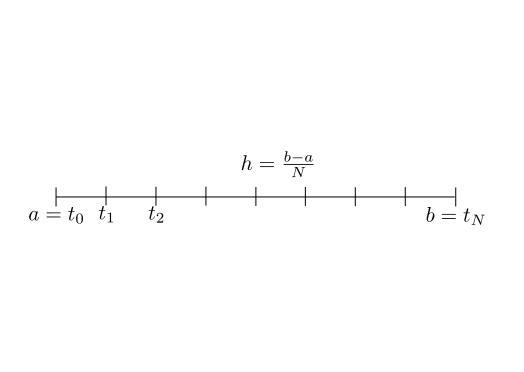
\includegraphics[width=\textwidth]{images/knoten_einschrittverfahren}
\caption{Der Zeitraum, in dem die DGL gelöstwerden soll, wird durch Knoten in Intervalle unterteilt. Knoten: $ t_i = a + jh, 0 \leq j \leq N $, $N=$ Anzahl Maschen, Schrittweite $h=\frac{b-a}{N}$}
\end{figure}


Wir betrachten hierzu die Integralgleichung für $y(t)$ auf $[t_j,t_{j+1}]$

$$y(t_{j+j})=y(t_j)+ \int^{t_{j+1}}_{t_j} y'(t) dt=y(t_j)+ \int^{t_{j+1}}_{t_j} f(t,y(t))dt$$

$f(t,y(t))$ ist unbekannt, weil $y(t)$ unbekannt ist. Also muss das Integral \emph{approximiert} werden. Durch die Apprximation des Integrals (durch Interpolation bzw. Approximation) berechnen wir die \emph{Näherung der Lösung} $$y_j \approx y(t_j), j=0,\ldots N$$

Durch die Approximation kommt es zum sogenannten \emph{Diskretisierungsfehler}, mit dem wir uns später noch ausführlicher befassen werden.

\begin{defi}[Disktretisierungsfehler $e_j$]
Der Diskretisierungsfehler $e_j$ berechnet sich durch $$e_j = y(t_j)-y_j$$
\end{defi}

Je nach Approximation des Integrals ergeben sich verschieden Verfahren, wobei wir nur Einschrittverfahren betrachten.

\begin{defi}[Einschrittverfahren]
Bei einem Einschrittverfahren basiert die Berechnung von $y_{j+1}$
\begin{itemize}
\item \emph{im expliziten Fall} nur auf den Werten von $y_j$
\item \emph{im impliziten Fall} nur auf den Werten von $y_j$ und $y_{j+1}$
\end{itemize}
\noindent Sobald Werte $y_{j-2}$ oder Werte die noch weiter in der "Vergangenheit" liegen berücksichtigt werden, spricht man von einem Zwei- bzw. Mehrschrittverfahren.
\end{defi}


Beim \emph{Euler Verfahren} macht man folgende Kette von Approximationen:
\begin{eqnarray*}
\int^{t_{j+1}}_{t_j} f(t,y(t))dt & \approx & \int^{t_{j+1}}_{t_j} f(t_j,y(t_j))dt \\
 & \approx & h \cdot f(t_j,y(t_j)) \\
 & \approx & h \cdot f(t_j,y_j)
\end{eqnarray*}


Anmerkung: Hier haben wir die Rechtechformel angewendet: $\int_{t_j}^{t_{j+1}}g(t)dt \sim h \cdot g(t_j)$ 
Für Abschätzungen des Integrationsfehlers muss $g(t)$ hinreichend glatt sein und $h$ hinreichend klein sein.

\begin{figure}[H]
\includegraphics[width=\textwidth]{images/rechteckformel-links}
\caption{Blauer Bereich ist der Integrationsfehler. Der rote Bereich ist das Ergebnis der numerische Integration mit der Rechtecksapproximation und die Summe von rotem und blauben Bereich ist das Ergebnis der exakten Integration}
\end{figure}


\begin{defi}[explizites Eulerverfahren]
\begin{equation*}
y_{j+1}=y_j+hf(t_j,y_j), ~j=0,...,N-1
\end{equation*}

Interpretation: Da $f(t_j,y_j)=y'(t_j)$ können wir für die Berechnung von $y_{j+1}$ einfach der Tangente durch $y_j$ mit der Steigung $f(t_j,y_j)$ folgen. Das tun wir solange, bis wir beim Zeitpunkt $t_{j+1}$ ankommen, was dem Zeitintervall $h$ entspricht. Also wie bereits definiert $y_j + h\cdot f(t_j,y_j) = y_{j+1} $
\end{defi}

%Die Qualität eines numerische Verfahren für ein AWP wird gemessen durch den Diskretisierungsfehler
%
%\begin{defi}[Diskretisierungsfehler]
%\begin{equation*}
%e_j=y(t_j)-y_j, ~1 \leq j \leq N 
%\end{equation*}
%
%\end{defi}
%
%Da $y(t)$ nicht bekannt ist ist das eine nicht berechenbare Grösse. Sie hängt allerdings eng mit dem berechenbaren \emph{lokalen Diskretisierungsfehler} zusammen (dazu später)

Ein weiteres auf der Rechteckregel basierendes Verfahren ist das \emph{implizite Eulerverfahren}. Hier wird $f(t_{j+1},y_{j+1})$ für die Approximation genutzt. Wir benutzen also den "rechten" Wert bei $t_{j+1}$ für die Berechnung des Integrals.

\begin{defi}[implizites Eulerverfahren]
\begin{equation*}
y_{j+1}=y_j+hf(t_{j+1},y_{j+1}), ~j=0,...,N-1
\end{equation*}

Anmerkung: Wer sich fragt, warum man überhaupt das implizite Eulerverfahren benutzen will, obwohl das explizite Eulerverfahren einfacher anzuwenden ist möge einen Blick auf Wikipedia werfen. Sinngemäß steht dort, dass das implizite Eulerverfahren ein größeres Stabilitätsgebiet hat.
\end{defi}

\begin{figure}[H]
\includegraphics[width=\textwidth]{images/rechteckformel-rechts}
\caption{der hellrote Bereich ist der Integrationsfehler. Der rote Bereich ist das Ergebnis der numerische Integration durch das Rechteckverfahren mit dem Wert bei $t_{j+1}$ als Stützstelle und der dunkelrote Bereich ist das Ergebnis der exakten Integration}
\end{figure}

Hier noch eine alternative Darstellung der Integrationsverfahren (nicht Teil der Vorlesung)

\begin{figure}[H]
\includegraphics[width=\textwidth]{images/eulers_compared}
\caption{Die Approximation durch den expliziten Euler ist in rot gehalten. Die Representation des impliziten Eulers ist blau. Der Grundgedanke beider Verfahren ist es, mit der Steigung $f(t_i,y_i)$ am Punkt $t_t$ bzw $t_{t+1}$ den Wert $y_{t+1}$ zu approximieren. Es ist offensichtlich, dass diese Approximationen nie dem genauen Wert von $y_{t+1}$ (in schwarz geschrieben) erreichen werden, es sei denn $y(t)$ ist linear.}
\end{figure}

\subsubsection{Kurzer Einschub über numerische Integration}
Wir benötigen genauere Verfrahen als die Rechteckregel.

Aufgabenstellung: Approximieren 


\begin{eqnarray*}
\int^{x+h}_{x} g(t) dt \\
x=t_j, ~ g(t)=f(t,y(t))
\end{eqnarray*}
$  $ und $g$ ausreichend glatt.

Gängiger Ansatz: Lege ein Gitter über $[x,x+h]$ mit $m\geq1$ Maschen und maschenweite $$\Delta = \frac{h}{m}$$ und benutze die Werte von g in den Gitterpunkten $$x+k\Delta, 0 \leq k \leq m$$

Ansatz: $$\int^{x+h}_{x} g(t) dt \approx h \sum^{m}_{k=0} w_k g(x+k\Delta)$$ wobei $$w_k \in \mathbb{R}, w_k > 0$$ die \emph{Gewichtung} der zugehörigen Stützstelle $g(x+k \Delta)$ ist. (Anmerkung: Es wäre rein theoretisch möglich auch negative Gewichtungen zu benutzen, das ist aber nicht erwünscht.) Je nach Wahl von $m$ und $w_k$ erhalten wir unterschiedliche Integrationsformeln.

Der Ansatz erhält wichtige Eigenschaften des Integrals, insbesondere die \emph{Linearität} $$\int\lambda_1g_1+\lambda_2 g_2 dt = \lambda_1 \int g_1 dt + \lambda_2 \int g_2 dt$$

die sich inder numerischen Quadraturformel wie folgt überträgt $$\sum^{m}_{k=0} \lambda_1 g_1(x+k\Delta) + \lambda_2 g_2(x+k\Delta) = \lambda_1 \sum^{m}_{k=0}  g_1(x+k\Delta) + \lambda_2 \sum^{m}_{k=0}  g_2(x+k\Delta) $$



Wir wollen nun Polynome möglichst hohen Grade mit dieser Quadraturformel \emph{exakt} integrieren. Wegen der Linearität der Formeln genügt es, eine Basis von Polynomen, etwas $1,t,t^{2},...,t^{q}$ zu benutzen, um ein Polynom vom Grad $\leq q$ zu integrieren. Um einfachere Formeln zu erhalten, benutzen wir im Folgenden die Basis $$1,t-x, (t-x)^{2},..., (t-x)^{q}$$

% Einsetzen: $\int^{x+h}_{x}1dt=h$ $h \sum^{m}_{k=0} w_k \cdot \underbrace{1}_{g(x+k\Delta) für g=1} = h \sum^{m}_{k=0} w_k $ Aus diesen Gleichunge folgt $\sum^{m}_{k=0} w_k  =1$


Für $g(t)=t-x$ $$\int^{x+h}_{x} (t-x) dt=\left. \frac{(t-x)^{2}}{2} \right|^{x+h}_x = \frac{h^{2}}{2} \Rightarrow \sum^{m}_{k=0} k w_k \stackrel{!}{=} \frac{h^{2}}{2\Delta h} = \frac{h}{2\Delta} \stackrel{\Delta = \frac{h}{m}}{=}  \frac{m}{2}$$


Allgemein für $g(t)=(t-x)^{q}, q \in \mathbb{N}_{0}$

\begin{eqnarray*}
&&\int^{x+h}_{x} (t-x)^{q} dt = \left. \frac{(t-x)^{q+1}}{q+1} \right|^{x+h}_x = \frac{h^{q+1}}{q+1} \\
&&\Rightarrow h \sum^{m}_{k=0} w_k (k\Delta)^{q} \stackrel{!}{=} \frac{h^{q+1}}{q+1} \\ 
&&\Leftrightarrow \sum^{m}_{k=0} k^{q} w_k = \frac{h^{q}}{(q+1)\Delta^{q}}\stackrel{ \Delta=\frac{h}{m}}{=}\frac{m^{q}}{q+1} \\
&& \Rightarrow  \sum^{m}_{k=0}k^{q} w_k = \frac{m^{q}}{q+1}
\end{eqnarray*}








%======================================== 06.05.2013

Für die numerische Integration $$\int_{x}^{x+h} g(t) dt \approx h \sum_{k=0}^{m} \omega_k g(x+k\Delta), \Delta=\frac{h}{m}$$ gilt also

$$ g(t)=(t-x)^{q} \text{wird exact integrert} \Leftrightarrow \underbrace{\sum_{k=0}^{m}k^{q}\omega_k=\frac{m^{q}}{q+1}}_{ \text{lineare Gleichungen für} ~ \omega_k}, q=0,1,2,\ldots$$

Es gibt zwei Mögliche Vorgehensweisen zur Bestimmung der $w_k$
\begin{itemize}
\item Wähle m und bestimme die $\omega_k$ aus den Gleichungen für $q=0,\ldots,m$
\item Wähle m, interpoliere $$(x,g(x)),(x+\Delta,g(x+\Delta)),\ldots,(x+h,g(x+h))$$ durch ein Polynom $p_m$ m-ten Grades und verwende $$\int_{x}^{x+h} g(t) dt \approx \int_{x}^{x+h} p_m(t) dt$$
\end{itemize}

\begin{bsp}[Bestimmung der Gewicht $\omega_k$ bei $m=1$]
$m=1 \Rightarrow \omega_0, \omega_1$

Ersten Vorgehensweise

$q=0$: $\omega_0 + \omega_1 \stackrel{!}{=} 1$

$q=1$: $0 \cdot \omega_0 + 1\cdot \omega_1 \stackrel{!}{=} \frac{1}{2}$ 

$\Rightarrow \omega_1=\frac{1}{2}$ 

$\Rightarrow \omega_2=\frac{1}{2}$

Dies liefert die bekannte Trapezregel: $$\int_{x}^{x+h} g(t) dt \approx h \cdot \frac{g(x)+g(x+h)}{2}$$

Die Bedingung für $q=2$ wird nicht mehr erfüllt $$0^{2}\cdot\omega_0 +1^{2}\cdot\omega_1=\frac{1}{2} \not= \frac{1}{3}$$

Zweite Vorgehensweise: wir interpolieren $(x,g(x))$ und $(x+h,g(x+h))$ durch ein Polynom ersten Grades (das ist eine Gerade)
$$g_1(t) = g(x) + \frac{g(x+h)-g(x)}{h} (t-x)$$
und integrieren

\begin{eqnarray*}
\int_{x}^{x+h} g_1(t) dt &=& h g(x) + \frac{g(x+h)-g(x)}{h} \left[ \frac{(t-x)^{2}}{2} \right]_{x}^{x+h} \\
&=& h g(x) + \frac{g(x+h)-g(x)}{h} \frac{h^{2}}{2} \\
&=& h \left( \underbrace{\frac{1}{2}}_{=\omega_0} g(x) + \underbrace{\frac{1}{2}}_{=\omega_1} g(x+h) \right)
\end{eqnarray*}

\end{bsp}

\begin{bsp}[Bestimmung der Gewicht $\omega_k$ bei $m=2$]
Wir wählen $$m=2, ~ \omega_0=0, \omega_1=1, \omega_2=0$$

Prüfen der Gleichungen:

$q=0$: $0+1+0=1$

$q=1$: $0\cdot0+1\cdot1+2\cdot0=1=\frac{2}{2}$

$q=2$: $0^{2}\cdot 0+1^{2}\cdot 1+ 2^{2}\cdot 0=1\not= \frac{4}{3} \Rightarrow $ nicht mehr erfüllt

Wir erhalten hier die Mittelpunktsregel $$\int_{x}^{x+h}g(t)\approx h \cdot g(x+\frac{h}{2})$$

Mit der Mittelpunktregel sind wir also genau so gut wie mit der Trapezregel, müssen aber nur an einem Punkt auswerten.
\end{bsp}

\begin{defi}[Ordnung eines Integrationsverfahrens]
Ein Integrationsverfahren hat die Ordnung $p \in \mathbb{N}$, falls gilt:

$$|\int^{x+h}_{x} g(t) dt - h \sum^{m}_{k=0} \omega_k g(x+k\Delta)| = O(h^{p+1})$$ mit $h \rightarrow 0$ für $g \in \mathbb{C}^{\infty}$
\end{defi}

Man erhält folgende gängien Integrationsrechgeln:

\begin{table}[H]
\centering
\begin{tabular}{ |c c c c c| }
\hline
  m & Name & Gewichtungen & Ordnung & Fehler \\
  \hline \hline
  1 & Trapezregel & $\frac{1}{2},\frac{1}{2}$ & 2 & $O(h^{3})$\\
  2 & Simpsonregel & $\frac{1}{6},\frac{4}{6},\frac{1}{6}$ & 4 & $O(h^{5})$\\
  3 & 3/8-Regel & $\frac{1}{8},\frac{3}{8},\frac{3}{8},\frac{1}{8}$ & 4 & $O(h^{5})$\\
  4 & Milne-Regel & $\frac{7}{90},\frac{32}{90},\frac{12}{90},\frac{32}{90},\frac{7}{90}$ &6 & $O(h^{7})$\\
  \hline
\end{tabular}
\end{table}

Für $m\geq 7$ treten negative Gewichte auf und die Formeln werden numerisch ungünstig.

Bemerkung: Es besteht ein enger Zusammenhang zwischen dem Maximalgrad, für den Polynome von einem Integrationsverfahren exakt integriert werden und der Ordnung des Verfahrens:

Sei das Verfahren exakt für alle Polynome vom Grad $\leq p-1$, d.h. obige Bedingungen gelten für $q=0,\ldots , p-1$. Ist nun $g \in C^{p}([x,x+h])$ dann gilt mit Taylor-Entwicklung für $t \in [x,x+h]$:

 $$g(t)=\sum_{l=0}^{p-1} \frac{1}{l!} g^{(l)}(x)(t-x)^{l}+R(t), \; R(t)=\frac{1}{p!}g^{(p)}(\tau)(t-x)^{p}$$

wobei $\tau \in [x,t]$ geeigent ist. Ist $C$ eine Oberschranke von $|g^{(p)}|/p!$ auf $[ x,x+h ] $ , dann gilt $|R(t)| \leq C|t-x|^{p} \leq Ch^{p}$ für alle $t \in [x,x+h]$. Da das Polynom $g(t)-R(t)$ exakt integriert wird, folgt

$$\left| \int^{x+h}_{x} g(t)dt - h \sum_{k=0}^{m} \omega_k g(x+k\Delta)\right| = \left| \int^{x+h}_{x} R(t)dt - h \sum_{k=0}^{m} \omega_k R(x+k\Delta)\right| \leq 2 Ch^{p+1}$$ d.h. das Verfahren hat \emph{mindestens Ordnung $p$}

\subsubsection{wichtige Einschrittverfahren}
Ausgangspunkt für alle Einschrittverfahren ist
\begin{equation}
y(t_{j+1})=\underbrace{y(t_j)}_{\approx y_j}+\underbrace{ \int^{t_{j+1}}_{t_j} f(s,y(s)) ds}_{to~ be~ approximated}
\end{equation}

Mit der Trapezregel zum Beispiel, wird das Integral mit
\begin{equation}
\int^{t_{j+1}}_{t_j} f(t,y(t))dt \approx h \frac{f(t_j,y(t_j))+f(t_{j+1},y(t_{j+1}))}{2}
\end{equation}
approximiert.

\begin{figure}[H]
\includegraphics[width=\textwidth]{images/trapez_approximation}
\caption{Der blaue Bereich ist das Ergebnis der exakten Integration. Die durchsichtig-rot darübergelegte rote Fläche repräsentiert die Integration nach der Trapezregel.}
\end{figure}



\begin{defi}[Trapezregel]
\begin{equation*}
y_{j+1} = y_j + \frac{h}{2} \left(f(t_j,y_j)+f(t_{j+1},y_{j+1})\right)
\end{equation*}
Das Trapezverfahren ist ein implizites Verfahren, was für die praktische Anwendung ein Nachteil ist.
\end{defi}


Die numerische Approximation 
\begin{equation}
f(t_j,y(t_j)) \approx f(t_j,y_j)
\end{equation}

ist naheliegend. Wir müssen uns also noch Gedanken über die numerische Approximation von $y(t_{j+1})$ machen.





a) $y(t_{j+1}) \approx y_{j+1} \Rightarrow$ Trapezverfahren $y_{j+1} = y_j + h \frac{f(t_j,y_j)+f(t_{j+1},y_{j+1})}{2}$

diese Verfahren ist IMPLIZIT ($y_{j+1}$ kommt rechts vor)


b) $y_{j+1} \approx y_j + h \cdot f(t_j,y_j)$ ist das Ergebnis des expliziten Eulerverfarhen, ausgedrückt durch $y_j$

$\Rightarrow$ Verfahren von Heun $y_{j+1} = y_j + h \frac{f(t_j,y_j)+f(t_{j+1},y_{j}+h \cdot f(t_j,y_j))}{2}$

\begin{defi}[Das Verfahren von Heun]
$y_{j+1} = y_j + h \frac{f(t_j,y_j)+f(t_{j+1},y_{j}+h \cdot f(t_j,y_j))}{2}$

Oder anders ausgedrückt (bekannt als erstes Runge-Kutta-Verfahren zweiter Ordnung)


$y_{j+1}=y_j + \frac{h}{2} (k_1 + k_2)$

$k_1=f(t_j,y_j)$

$k_2=f(t_{j+1},y_j+hk_1)$

Das Verfahren von Heun basierst auf der Trapezregel, wobei $y_{y+1}$ durch das explizite Eulerverfahren approximiert wird!
\end{defi}


%==================================== vorlesung 7.5.2013

Weiteres Verfahren durch Mittelpunktregel

\begin{eqnarray*}
\int_{t_j}^{t_{j+1}} f(t,y(t)) dt & \approx & h \cdot f(t_j + \frac{h}{2},y(t_j+\frac{h}{2})) \\
 &\underbrace{\approx}_{y(t_j+\frac{h}{2}) \approx y_j + \frac{h}{2}f(t_j,y_j)}&  h\cdot f(t_j+\frac{h}{2},y_j+\frac{h}{2}f(t_j,y_j))
\end{eqnarray*}



Somit modifiziertes EulerVerfahren
$y_{t_j+1} = y_j+h\cdot f(t_j+\frac{h}{2},y_j+\frac{h}{2}f(t_j,y_j))$


\begin{defi}[Modifiziertes Eulerverfahren]

$$y_{j+1}=y_j+h\cdot f(t_j+\frac{h}{2},y_j+\frac{h}{2} f(t_j,y_j))$$

(bekannt als zweites Runge-Kutta-Verfahren zweiter Ordnung)

$$y_{j+1}=y_j + h k_2$$ 

mit $k_1=f(t_j,y_j),k_2=f(t_j + h/2, y_j + (h/2)k_1)$

\end{defi}




Verwenden wir die Simpson-Regel 

\begin{defi}[Simpsonregel]
\begin{equation*}
\int_{t_j}^{t_{j+1}} f(t,y(t)) dt \approx \frac{h}{6} \left(f(t_j,y_j)  + 4 \cdot f(t_j + \frac{h}{2},y(t_j + \frac{h}{2})) + f(t_{j+1},y_{j+1}) \right)
\end{equation*}
Das Simpsonverfahren ist ein implizites Verfahren, was für die praktische Anwendung ein Nachteil ist.
\end{defi}

und approximieren wir 

$y(t_j+0.5\cdot h)$ und $y(t_{t_j+1})$ geeignet durch Taylorentwicklung, dann erhalten wir das wichtige Runge-Kutta-Verfahren (RK4)

\begin{defi}[Das Runge-Kutta-Verfahren vierter Ordnung (RK4)]
\begin{eqnarray}
y_{j+1}&=& y_j+\frac{h}{6}(k_1+2k_2+2k_3+k_4) \\
&& k_1=f(t_j,y_j) \nonumber \\
&& k_2=f(t_j+\frac{h}{2},y_j+\frac{h}{2}k_1) \nonumber\\
&& k_3=f(t_j+\frac{h}{2},y_j+\frac{h}{2}k_2) \nonumber\\
&& k_4=f(t_{j+1},y_j+h\cdot k_3) \nonumber
\end{eqnarray}
\end{defi}

Man beachte, dass die Gewichtungen denen des Simpsonverfahrens ähneln und auch tatsächlich mit diesen verwandt sind!

Beobachteunge aus numerischen Beispielen in der Vorlesung:

\begin{table}[H]
\centering

\begin{tabular}{ |l c| }
	\hline
  Verfahren & Diskretisierungsfehler \\ \hline \hline
  Euler & $O(h)$\\
  Heun & $O(h^{2})$ \\
  mod. Euler & $O(h^{2})$ \\
  RK4 & $O(h^{4})$ \\ \hline
\end{tabular}
\end{table}

Im offiziellen Skript befinden sich noch zwei grössere Beispiel zur numerischen Berechnung von DGLs, die aber in der Vorlesung nicht behandelt wurden.

Aber wie geht nun die mathematische Berechnung des Diskretisierungsfehlers?

\subsubsection{Konvergenz und Konsistenz}

Vereinheitlichte Notation für Einschrittverfahren

\begin{equation}
y_{j+1} = y_j + h \Phi (t_j, h_i y_j)
\end{equation}

\begin{defi}[Verfahrensfunktion von Einschrittverfahren]

Die Funktion 

\begin{equation*}
\Phi(t,h,y)
\end{equation*}
heisst Verfahrensfunktion

Kann $\Phi$ explizit (d.h. formelmäßig) berechnet werden, dann ist das Verfahren emplizit, ansonsten implizit.
\end{defi}

\begin{bsp}[Verfahrensfunktion des Eulerverfahren]


$y_{j+1}=y_j+h\underbrace{f(t_j,y_j)}_{\Phi(t_j,h,y_j)} \Rightarrow \Phi(t_j,h,y_j)=f(t_j,y_j)$


\end{bsp}

\begin{bsp}[Verfahrensfunktion des Verfahren von Heun]



$y_{j+1}=y_j+ \underbrace{\frac{h}{2} (f(t_j,y_j) + f( \underbrace{t_j+h}_{t_{j+1}},y_j+hf(t_j,y_j)))}_{h\Phi(t_j,h,y_j)}$

$\Rightarrow \Phi(t,h,y)=\frac{1}{2}(f(t,y)+f(t+h,y+hf(t,y)))$
\end{bsp}


\begin{bsp}[Verfahrensfunktion des mod. Euler]



$ \Phi(t,h,y)=f(t+\frac{h}{2},y+\frac{h}{2}f(t,y))$
\end{bsp}



\begin{bsp}[Verfahrensfunktion des impliziten Euler]

\begin{equation*}
y_{j+1}=y_j+hf(t_j+h,y_{j+1})
\end{equation*}

\begin{eqnarray*}
\Rightarrow \Phi(t_j,h,y_j)&=&f(t_j+h,y_{j+1}) \\
&=& f(t_j+h,y_j+h\Phi(t_j,h,y_j))
\end{eqnarray*}


$\Phi(t,h,y)$ ist implizit gegeben durch die Gleichung. Daher ist dieses Verfahren ein implizites Verfahren.
\end{bsp}


Folgende abschätzbare Grösse ist eng verknüpft mit den nicht  direkt abschetzbaren Diskretisierungsfehler

\begin{defi}[Konsistenzfehler eines Verfahrens]

Der Ausdruck

$\tau(t,h)=\frac{1}{h}(y(t+h)-y(t)-h\Phi(t,h,y(t)))$ mit $y(t)=Loesung$

heisst \emph{lokaler Abbruchfehler} oder \emph{Konsistenzfehler} des Verfahren an der Stelle $t$

\end{defi}


Es gibt  zwei Interpretationen von $\tau(t,h)$:

\begin{itemize}
\item $\tau(t,h) = \frac{1}{h} \cdot$ (Defekt bei Einsetzten der Lösung in die Verfahrensgelichung)
\item $\tau(t,h) = $ Differenz der Sekantensteigung der Lösung auf $[t,t+h]$ und der Sekantensteigung der numerischen Lösung
\end{itemize}

Zur Veranschaulichung der zwei Interpretationen
\begin{figure}[H]
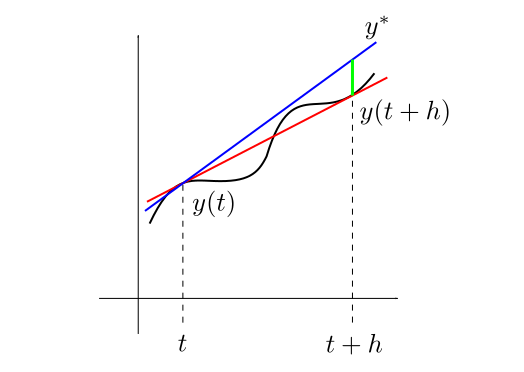
\includegraphics[width=\textwidth]{images/konsistenzfehler}
\caption{Grün ist der Konsistenzfehler des Verfahrens. $y*$ ist die Lösung des numerischen Verfahrens, das von der echten Lösung an $y(t+h)$ abweicht.}
\end{figure}


Sekantensteigung der Lösung y $\frac{y(t+h)-y(t)}{h}$

Sekantensteigung der num. Lösung $\frac{y^{*}-y(t)}{h}=\Phi(t,h,y(t))$


\begin{defi}[Konsistenzordnung eines Verfahrens]
Das Verfahren mit Verfahrensfunktion $\Phi$ heisst konsistent von der Ordnung $p \in \mathbb{N}$ falls mit einer konstanten $C>0$ gilt:


$|\tau(t,h)| \leq C h^{p}$ auf $[a,b]$ für h hinreichend klein

\end{defi}
\begin{defi}[Stabilität eines Verfahrens]
Das Verfahren heisst stabil falls es auf $K>0$ gibt mit

$|\Phi(t,h,y_1)-\Phi(t,h,y_2)| \leq K|y_1-y_2|$ für alle $t\in [a,b]$ und alle $y_1,y_2$

\end{defi}

\begin{defi}[Konvergenzordnung eines Verfahren]
Das Verfahren heisst konvergent mit der Ordnung $p$, falls es $M>0$ und $H>0$ gibt mit

$|e_j|=|y(t_j)-y_j|\leq Mh^{p}, ~ \forall j=1, \ldots , N$ auf alle N mit $h=\frac{b-a}{N} \leq H$
\end{defi}


Bemerkung: Stabilität ist eine Lipschitzbedingung bezüglich y für $\Phi$ Diese folgt überlicherweise aus der Lipschitzstegikeit bezüglich y von f.

Zentral ist folgender Satz

\begin{satz}[Zusammenhang zwischen Konsistenzordnung und Konvergenzordnung]

Ein stabiles, konsistentes Verfahren ist konvergent. Ist die Konsistenzordnung p, so ist auch die Konvergenzordnung p.

\end{satz}


\begin{bsp}[Konsistenzordnung des Eulerverfahren]



$f \in C^{1}([a,b]\times \mathbb{R})$ mit y als Lösung von $y'=f(t,y) \Rightarrow y' ~ ist ~ C^{1} \Rightarrow y ~ ist~ c^{2}$

Taylor

$y(t+h)-y(t)=y'(t)\cdot h + \frac{1}{2} y''(t+\underbrace{\psi}_{\in [0,1] geeignet} h)h^{2} = f(t,y(t))h+\frac{1}{2}y''(t+\psi h)h^{2}$

$\Rightarrow |\tau(t,h)|=\left|  \frac{y(t+h)-y(t)}{h} - \Phi(t,h,y(t))   \right| = \frac{1}{2}|y''(t+\psi h)|h = O(h)$

$\Rightarrow$ Konsistenzordung $p=1$


\end{bsp}


%========================================= Mitschrift vom 13.5.2013
Konsistenzfehler
$\tau(t,h)=\frac{y(t+h)-y(t)}{h} -\Phi(t,h,y(t))$

Konsistenzordnung $p$, falls
$|\tau(t,h)|=O(h^{p}), ~(h \rightarrow 0)$

\begin{bsp}[Modifiziertes Euler-Verfahren]
$\Phi(t,h,y)=f(t+\frac{h}{2},y+\frac{h}{2}f(t,y))$

\begin{eqnarray*}
y(t+h)&\stackrel{Taylor ~ um ~ h=0}{=}& y(t)+y'(t)h+\frac{1}{2}y''(t)h^{2}+\overbrace{\frac{1}{6}y'''(t + \underbrace{\xi}_{ \in [0,1]} h) h^{3}}^{R_3 = O(h^{3})} \\
&=& y(t)+f(t,y(t))h + \frac{1}{2}(f_t + f_y \cdot f)h^{2}+R_3
\end{eqnarray*}

\begin{eqnarray*}
\Phi(t,h,y(t))&=&f(t+\frac{h}{2},y(t)+\frac{h}{2}f(t,y(t))) \\
&\stackrel{Taylor}{=}& f(t,y(t))+ \underbrace{f_t \cdot \frac{h}{2} + f_y \frac{h}{2}f(t,y(t))}_{\nabla_{t,y}f(t,y(t))^{T}}
\begin{pmatrix}
\frac{h}{2} \\
\frac{h}{2} f(t,y(t))
\end{pmatrix}
\end{eqnarray*}

\begin{eqnarray*}
|\tau(t,h)|&=&\left| \frac{y(t+h)-y(t)}{h} - \Phi(t,h,y(t))\right|\\
& =& \left| f+\frac{1}{2}f_t h + \frac{1}{2}f_y f h + \frac{1}{h}R_3 -\left( f + f_t \frac{1}{2}+f_y \frac{h}{2} + R_2 \right)\right| \\
&=& \left| \frac{1}{h}R_3 - R_2\right| \\
& =&  O(h^{2})
\end{eqnarray*}

$\Rightarrow$ Konsistenzordnung mind $p=2$

Nebenrechung:
$f(t+\underbrace{s}_{\frac{h}{2}},\underbrace{y}_{y(t)}+\underbrace{d}_{\frac{h}{2} f}) = \nabla f(t,y)^{T} \begin{pmatrix}
s \\ d
\end{pmatrix} + O \left( \left|\left| \begin{pmatrix}
s \\ d
\end{pmatrix} \right|\right|^{2} \right)
$
\end{bsp}

Konsistenzordnung einiger Verfahren:
\begin{table}[H]
\centering
\begin{tabular}{|l c|}
\hline
Verfahren & Konsistenzordnung \\
\hline \hline
Expl. Euler-Verf. & 1 \\
Impl. Euler-Verf. & 1 \\
Verf. von Heun & 2 \\
Mod. Euler & 2\\
RK4 & 4 \\
\hline
\end{tabular}
\end{table}

\subsubsection{Explizite Runge-Kutta-Verfahren}
Explizite RK-Verfahren haben folgende Form:

r-stufiges explizites Runge-Kutta-Verfahren:

\begin{equation}
k_i=f(t+\gamma_i h, y + \sum\limits_{j=1}^{i-1} \alpha_{ij}k_j), \; i=1,\ldots, r
\end{equation}

\begin{equation}
\Phi(t,h,y)=\sum_{i=1}^{r} \beta_i k_i
\end{equation}


Bezeichnung: $k_i=k_i(t,h,y)$ heist $i$-te Stufe.

Kompakte Darstellung als \underline{ Butcher-Schema}

\begin{table}[H]
\centering
\begin{tabular}{c| c c c c c}
$\gamma_1$ & 0 \\
$\gamma_2$ & $\alpha_{21}$ & 0 \\
$\gamma_3$ & $\alpha_{31}$ & $\alpha_{32}$ & 0\\
$\vdots$ & $\vdots$ & $\vdots$ & $\ddots$ & $\ddots$ \\
$\gamma_r$ & $\alpha_{r1}$ & $\alpha_{r1}$ & \ldots & $\alpha_{r,r-1}$ & 0 \\
\hline \\
 & $\beta_1$ & $\beta_1$ & \ldots & $\beta_{r-1}$ & $\beta_r$
\end{tabular}
\caption{Man beachte, dass bei expliziten RK-Verfahren alle $\alpha_{ij}$ auf der Diagonale und oberhalb davon gleich Null sind.}
\label{tab:ExplicitRkButscherScheme}
\end{table}



\begin{bsp}[Butcher-Schema Expliziter Euler]
$r=1$
\begin{table}[H]
\centering
\begin{tabular}{c| c}
0 & 0\\
\hline
& 1
\end{tabular}
\end{table}
\end{bsp}

\begin{bsp}[Butcher-Schema Mod Euler]
$r=2$
\begin{table}[H]
\centering
\begin{tabular}{c| c c}
0 & 0 &\\
$\frac{1}{2}$ & $\frac{1}{2}$ & 0 \\
\hline \\
 & 0 & 1
\end{tabular}
\end{table}
\end{bsp}

\begin{bsp}[Butcher-Schema Von Heun]
$r=2$
\begin{table}[H]
\centering
\begin{tabular}{c| c c}
0 & 0 &\\
1 & 1 & 0 \\
\hline \\
 & $\frac{1}{2}$& $\frac{1}{2}$
\end{tabular}
\end{table}
\end{bsp}

\begin{bsp}[Butcher-Schema Trapezregel]
$r=2$
\begin{table}[H]
\centering
\begin{tabular}{c| c c}
0 & 0 &\\
1 & $\frac{1}{2}$ & $\frac{1}{2}$ \\
\hline \\
 & $\frac{1}{2}$& $\frac{1}{2}$
\end{tabular}
\end{table}
\end{bsp}


\begin{bsp}[Butcher-Schema RK4]
$r=4$
\begin{table}[H]
\centering
\begin{tabular}{c| c c c c}
0 & 0 &\\
$\frac{1}{2}$ & $\frac{1}{2}$ & 0 \\
$\frac{1}{2}$ & 0 & $\frac{1}{2}$ & 0 & \\
1 & 0 & 0 &1 & 0 \\
\hline \\
 & $\frac{1}{6}$ & $\frac{1}{3}$ & $\frac{1}{3}$ & $\frac{1}{6}$
\end{tabular}
\end{table}
\end{bsp}




%================================= 27.5.2013 (Vorelsung von Asissiten, nicht Prof)

Anmerkung: Ein bisschen Wiederholung (die folgende Vorlesung wurde nicht von Prof. Ulbrich gehalten)

Explizites Runge-Kutta-Verfahren
$$\varphi(t,h,y) = \sum^{r}_{i=1} \beta_i k_i$$

(r-stufig)

$$k_i = f(t+\gamma_i h, y + h \sum^{i-1}_{j=1} \alpha_{ij}k_j$$

Im Butcherschema heisst das, dass alle $\alpha_{ij}$ oberhalb der Diagonale gleich Null sind.

\begin{bsp}[Butcherschema für das Verfahren von Heun]

Verfahren von Heun

$$\varphi(t,h,y) = \frac{1}{2}(f(t,y)+f(t+h,y+f(t,y))) \stackrel{!}{=} \frac{1}{2}k_1 + \frac{1}{2}k_2$$

$$\Rightarrow k_1 = f(t,y) = f(t + 0 \cdot h,y)$$

$$\Rightarrow k_2 = f(t+h,y+hk_1)=f(t+1 \cdot h,y+hk_1)$$

\begin{table}[H]
\centering
\begin{tabular}{c| c c}
0 & 0 &\\
1 & 1 & 0 \\
\hline \\
 & $\frac{1}{2}$& $\frac{1}{2}$
\end{tabular}
\end{table}


\end{bsp}


Mit diesem Ansatz lassen sich RK-Verfahren beliebiger Konsistenzordnung $p$ erzeugen. Man muss dafür die Stufenzahl $r$ gross genug wählen (bis zur Stufe 4 ist der Verhältnis lienar, danach muss man immer mehr Stufen benutzen um die Konsistenzordnung zu verbessern)

\begin{satz}[Konsistenzordnung expliziter RK-Verfahren]
Betrachte ein $r$-stufiges, explizites RKV mit $$\gamma_i = \sum^{r}_{j=1} \alpha_{ij}, i=1, \ldots , r$$

Es besitzt genau dann für jede rechte Seite $f \in C^{p}([a,b]\times \mathbb{R})$ die Konsistenzordnung


\begin{eqnarray*}
p \geq 1 &\Leftrightarrow & \sum^{r}_{i=1} \beta_i=1 \\
p \geq 2 & \Leftrightarrow & \sum^{r}_{i=1} \beta_i \gamma_i =\frac{1}{2}\\
p \geq 3 & \Leftrightarrow & \sum^{r}_{i=1} \beta_i \gamma_i^{2} =\frac{1}{3}\\ &\text{und}& \sum^{r}_{i,j=1} \alpha_{ij} \beta_i \gamma_i =\frac{1}{6}\\
p \geq 4 & \Leftrightarrow & \sum^{r}_{i=1} \beta_i \gamma_i^{3} =\frac{1}{4} \\
& \text{und}& \sum^{r}_{i,j=1} \alpha_{ij} \beta_i \gamma_i \gamma_j =\frac{1}{8}     \\ &\text{und} &\sum^{r}_{i,j=1} \alpha_{ij} \beta_i  \gamma_j^{2} =\frac{1}{12} \\
& \text{und}& \sum^{r}_{i,j,k=1} \alpha_{ij} \beta_i \alpha_{ik} \gamma_k =\frac{1}{24}
\end{eqnarray*}



\end{satz}


\subsubsection{Bermerkungen}

Durch eine \emph{adaptive, zeitabhängige Wahl der Schrittweite} $h$ lässt sich der Aufwand der Verfahren stark verringern. Die Steuerung der Schrittweite erfordert eine Schätzung des \emph{lokalen Fehlers}.

Es gibt zwei Möglichkeiten:

\begin{enumerate}
\item Hierzu verwendet man ein Verfahren mit zwei unterschiedlichen Schrittweiten (z.B. $h$ und $\frac{h}{2}$) und vergleicht das Resultat.
\item Man verwendet Verfahren unterschiedlicher Ordnung.

\end{enumerate}



\subsubsection{Steife Differentialgelichungen}
Steife DGLs kommen nur bei mehrdimensionalen Probleme vor. Der schnell fallende Teil der Lösung Lösung ist an sich für das Gesamtergebnis nicht wichtig, zwingt den numerischen Lösungsalgorithmus aber dazu, kleine Approximationsschritte zu machen. (Der aufmerksame Student bemerkt hier sofort die Parallelen zu Regelungssysteme 1, insbesondere Buss-Skript Kapitel 5.8)

\begin{figure}[H]
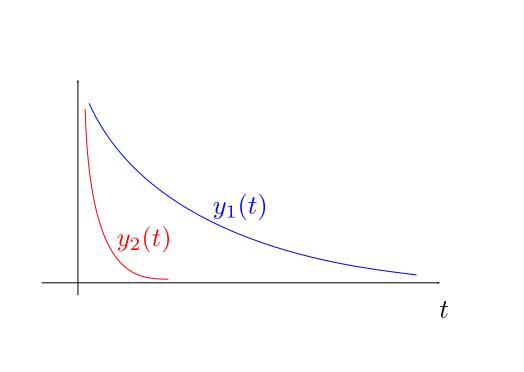
\includegraphics[width=\textwidth]{images/steife_dgl}
\caption{Der schnell abklingende, rote Teil der Lösung spielt bei der Gesamtlösung kaum eine Rolle (mit zunehmendenm $t$ verringert sich sein Anteil an der Lösung). Trotzdem zwingt die hohe Änderungsrate von $y_2(t)$ zu kleinen Integrationsschritten.}
\end{figure}


Ausgangsfunktion:

$$y'(t) = f(t,y(t)), t\in [a,b]$$

$$y(0)=y_0$$

$$y \in \mathbb{R}^{n}, f:[a,b] \times \mathbb{R}^{n} \rightarrow \mathbb{R}^{n}, n > 1$$

Der Begriff "steifes DGL-System" ist nicht einheitlich definiert, der wesentliche Punkt aller steifen DGL-System ist jedoch: \emph{ die Lösung ist zusammengesetzte aus langsam veränderlichen Teilen (die meist Abklingen) und Teilen, die im Vergleich dazu schnell abklingen.}

\begin{defi}[Steife eines Systems]
Ein System heisst \emph{steif}, wenn gewissen Anteile der Lösung \emph{sehr viel schneller} abklingen als andere. 
\end{defi}



%=============================== Vorlesung 28.5.2013 - ned on Ulbrich



Wichtiger Spezialfall: Lineare AWP

$$y'=Ay(t)+g(t), t \in [a,b], y(0)=y_0$$

$$A \in \mathbb{R}^{n \times n}, g:[a,b] \rightarrow \mathbb{R}^{n}, y: [a,b] \rightarrow \mathbb{R}^{n}$$

Sei $A$ diagonalisierbar mit den Eigenwerten $\lambda_i$ und den Eigenvektoren $v_i$. Mit einer partikulären Lösung $y_p(t)$ ist dann die allgemeine Lösung $$y(t)=y_h(t)+y_p(t)$$ wobei $$y_h(t)=\sum_{i=1}^{n}c_i e^{\lambda i t}v_i$$

Für den Fall $Re\{\lambda_i\}<0, i=1,\ldots,n$ konvergiert $e^{\lambda i t} \rightarrow 0 ~ (t\rightarrow \infty)$ $$ \Rightarrow y(t) \stackrel{(t\rightarrow \infty)}{\rightarrow} y_p(t)$$

Hierbei klingen die Summanden in $y_h$ mit $Re\{\lambda_i\}<<0$ sehr schnell ab und Summanden mit $Re\{\lambda_i\}<0$ deutlich langsamer ab. Gibt es also Eigenwerten mit $Re\{\lambda_i\}<<0$ und Eigenwerte mit $Re\{\lambda_i\}<0$ (schwach negativer Realteil) so nennt man das DGL-System \emph{steif}.

Allgemeiner nichtlinearer Fall $y'=f(t,y)$:

Ein nichtlineares DGL-System heisst steif (in einer Umgebung von $(t,y)$), wenn die Jakobimatrix von $f$ Eigenwerte mit $Re\{\lambda_i\}<<0$ und $Re\{\lambda_i\}<0$ besitzt.

Problem an einem Bsp:

\begin{bsp}[$y'=Ay$]

$$y(0)=y_0 = \begin{pmatrix}
c_1+c_2 \\ c_1-c_2
\end{pmatrix}
$$


$$  A= \frac{1}{2}
\begin{pmatrix}
\lambda_1+\lambda_2 & \lambda_1-\lambda_2 \\
\lambda_1-\lambda_2 & \lambda_1+\lambda_2
\end{pmatrix} \text{mit} \lambda_2 << \lambda_1 < 0
$$

$$\Rightarrow \lambda_1, \lambda_2 \text{sind Eigenwerten von} A$$

$$
v_1=\begin{pmatrix}
1 \\ 1
\end{pmatrix}
v_2=\begin{pmatrix}
1 \\ -1
\end{pmatrix}
$$

$$
\Rightarrow y(t)=c_1 e^{\lambda_1 t} v_1 + c_2 e^{\lambda_2 t} v_2
$$

$\Rightarrow$ Der zweite Termin spielt nach kürzester Zeit keine Rolle mehr. Der erste Term ist bestimmend und konvergiert für $t \rightarrow \infty$ gegen Null.

$\Rightarrow$ Vin einem geeigneten Integrationsverfahren erwartet man, dass dieses Verhlaten ohne grosse Einschränkungen an der Schrittweite wiedergespiegelt wird

$\Rightarrow$ $y_i \rightarrow 0 (i \rightarrow \infty)$

Mit dem expliziten Euler ($y_0 = c_1 v_1 + c_2 v_2$)


$$y_{j+1} = y_j + hAy_j=B(h)y_j$$

$$\Rightarrow y_j = B(h)^{j}y_0 = c_1 B(h)^{j}v_1 + c_2 B(h)^{j}v_2 = c_1 (1+h\lambda_1)^{j}v_1 + c_2 (1+h\lambda_2)^{j}v_2$$

Damit $y_j \rightarrow 0$ muss $|1+h\lambda_1|<1$ und $|1+h\lambda_2|<1$, z.B. $\lambda_1 = -1, ~ \lambda_2=-1000$

$$ |1+h\lambda_1| = |1-h|<1 \Leftrightarrow h < 2$$

$$ |1+h\lambda_2| = |1-1000h|<1 \Leftrightarrow h < 0.0002$$

Ein für steife DLG geeigentes Verfahren sollte hier für alle $h<2$ $|y_j|\rightarrow 0$ liefern
\end{bsp}

\begin{bsp}[Nichtlinearer Fall]
Gradientenfluss einer Potentialfunktion

Die Rosenbrockfunktion
$$\Phi: \mathbb{R}^{2} \rightarrow \mathbb{R}$$

$$\Phi(x)=100(x_2-x_1^{2})+(1-x_1)^{2}$$

Richtung des Steilsten Abstiegs $-\nabla \Phi = f$

$$ f(x) = -\nabla \Phi(x) = \begin{pmatrix}
400 x_1(x_2-x_1^{2})+2(1-x_1)\\
200(x_1^{2}-x_2)
\end{pmatrix}
$$

Weg $x(t) \rightarrow$ Fluss des steilsten Abstiegs : $x'(t)=f(x(t))$

Betrachte Jakobimatrix von $f$

$$Jf(x)=\begin{pmatrix}
400x_2-1200x_1^{2}-2 & 400x_1 \\
400x_1 & -200
\end{pmatrix}
$$

Das "Tal" ist gegeben durch $x_2=x_1^{2}$

$\Rightarrow$ Jacobimatrix im "Tal" durch einsetzten von  $x_2=x_1^{2}$

$$
JF(x) = \begin{pmatrix}
-800x_1^{2} & 400x_1 \\
400 x_1 & -200
\end{pmatrix}
$$

Man berechne nun die Eigenwerte für verschieden $(x_1,x_2)$ besonders in Nähe des Tals.

$\Rightarrow$ Problem ist steif in der Nähe des Tals.

\end{bsp}

Die homogene Lösung einer linearen AWP ist für diagonalisierbares $A$ zusammengesetzt aus Linearkombinationen von $e^{\lambda_i t}v_i$

$\Rightarrow$ um Verfahren für steife DGL zu bewerten und zu analysieren, betrachtet man die folgende Modellgleichung (\emph{dahlquist'sche Testgleichung})

\begin{defi}[Dahlquist'sche Testgleichung]

\begin{equation}
y'=\lambda y 
\end{equation}

\begin{eqnarray*}
 y(0)=1, \\
 \lambda \in \mathbb{C}, Re\{ \lambda \} < 0
\end{eqnarray*}

Die Lösung ist $$y(t)=e^{\lambda t}$$ und wegen $Re\{ \lambda \} < 0 \Rightarrow \lim\limits_{t \rightarrow \infty} y(t)=0$

Forderung: Die numerisch gewonnenen Lösungen $y_j$ sollen dei Eigenschaften von $y(t)$ möglichst gut wiederspiegeln. Ich kann also mit dieser Gleichung die qualität eines numerischen Verfahrens testen.

\end{defi}

\begin{defi}[Stabilität]
Ein Verfahren heißt
\begin{description}
\item[A-stabil], wenn angewendet auf das Modellproblem die Lösungen $y_j$ die Bedingung $$|y_{j+1}| \leq |y_j| \forall j \geq 0, h > 0$$ erfüllt.
\item[L-stabil] wenn es A-stabil ist und zusätzlich $|y_j| \stackrel{j \rightarrow \infty}{\rightarrow} 0$
\end{description}
\end{defi}

Bei vielen Einschritt-Verfahren gilt bei Anwendung auf das Modellproblem der Zusammenhang über die \emph{Stabilitätsfunktion}

\begin{defi}[Stabilitätsfunktion R]

\begin{eqnarray*}
R&:&D \rightarrow \mathbb{C}\\ 
q&=&h\lambda \\
y_{j+1}&=&R(q) ~ y_j 
\end{eqnarray*}

\end{defi}

\begin{defi}[Stabilität als Funktion der Stabilitätsfunktion]
\begin{eqnarray*}
\text{A-stabil} &\Leftrightarrow &|R(q)| \leq 1 \forall q \in \mathbb{C}, Re\{ q\} < 0\\
\text{L-stabil}  &\Leftrightarrow & |R(q)| < 1 \forall q \in \mathbb{C}, Re\{ q\} < 0
\end{eqnarray*}
\end{defi}

\begin{defi}[Stabilitätsgebiet $S$]
$$S=\{q \in \mathbb{C} | ~ |R(q)|<1 \}$$
\end{defi}

\begin{satz}[Zusammenang Stabilitätsgebiet und L-Stabilität]
$$\text{L-stabil} \Leftrightarrow \{ q \in \mathbb{C} | Re\{ q\}<0 \} \subset S$$
\end{satz}

\begin{bsp}[Stabilität des expliziten Euler-Verfahrens]
\begin{eqnarray*}
y_{j+1}&=&y_j + hf(t_j,y_j)\\
& =& y_j + h \lambda y_j \\
&=& (1 + \lambda h)y_j 
\Rightarrow R(q) = 1 + q
\end{eqnarray*}

$$\Rightarrow S=\{ q \in \mathbb{C} | |1+q| < 1 \}$$


\begin{figure}[H]
\includegraphics[width=\textwidth]{images/stability_explicit_euler}
\caption{Das Stabilitätsgebiet des expliziten Euler-Verfahrens ist ein Kreis um $-1$ mit dem Radius $1$. Achtung, das Stabilitätsgebiet ist eine offene Menge, d.h. der Rand des Kreises ist nicht Teil von $S$.}
\end{figure}


Das Explizite Eulerverfahren ist \emph{nicht} A-stabil, und damit auch nicht L-stabil!

\end{bsp}


\begin{satz}[A-Stabilität expliziter RK-Verfahren]
Alle expliziten Runge-Kutta Verfarhen sind \emph{nicht} A-stabil!
\end{satz}

\begin{bsp}[Stabilität des impliziten Euler-Verfahrens]

\begin{eqnarray*}
y_{j+1}&=&y_j + hf(t_{j+1},y_{j+1}) \\
&=& y_j + h \lambda y_{j+1} \\
\Leftrightarrow y_{j+1} &=& \frac{1}{1-h\lambda} y_j\\
& \Rightarrow & R(q)=\frac{1}{1-q}
\end{eqnarray*}

$$S=\{q \in \mathbb{C}; |1-q|>1 \} \supset \{ q \in \mathbb{C}; Re(q)<0\}$$

TODO: Ich glaube die Graphik ist nicht ganz richtig.

\begin{figure}[H]
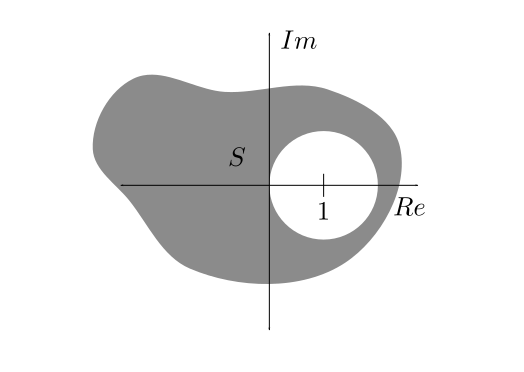
\includegraphics[width=\textwidth]{images/stability_implicit_euler}
\caption{Das Stabilitätsgebiet des impliziten Euler-Verfahrens ist die ganzen komplexe ebene $\mathbb{C}$ ohne den Kreis mit Radius $1$ um $1$. Der Rand des Kreises ist \emph{nicht} Teil von $S$.}
\end{figure}

Da die komplexe Halbebene $Re\{ q\}<0$ Teil von $S$ ist, mathematisch ausgedrückt $$\{ q \in \mathbb{C} | Re \{ q\}<0 \} \subset S$$

ist das implizite Eulerverfahren L-stabil!

Interpreation(aus praktischer Beobachtung): Des Verfahren ist sehr stabil. Manchmal sogar "zu" stabil (Erinnerung: in einer der Übungen wurde die approximation des Kreises zu stark gedämpft und die Funktion ist gegen Null konvergiert, anstatt auf dem Einheitskreis zu bleiben.)

\end{bsp}



\begin{bsp}[Stabilität des Trapez-Verfahrens]


\begin{eqnarray*}
y_{j+1}&=&y_j + \frac{h}{2} \left(f(t_{j},y_{j}) + f(t_{j+1},y_{j+1}) \right)  \\
&=&y_j + \frac{h}{2} f(t_{j},y_{j}) + \frac{h}{2} f(t_{j+1},y_{j+1})\\
&=& y_j +  \frac{h}{2} \lambda y_{j} + \frac{h}{2} \lambda y_{j+1} \\
\Leftrightarrow y_{j+1}- \frac{h}{2} \lambda y_{j+1} &=&  y_j +  \frac{h}{2} \lambda y_{j} \\
\Rightarrow y_{j+1}&=&\frac{1+\frac{h}{2} \lambda}{1-\frac{h}{2} \lambda} y_j\\
\Rightarrow R(q)&=& \frac{1+\frac{1}{2}q}{1-\frac{1}{2}q}
\end{eqnarray*}
Für das Stabilitätsgebiet $S$ muss wie wir beretis wissen, gelten



\begin{eqnarray*}
|R(q)|&<&1 \\
\left| \frac{1+\frac{1}{2}q}{1-\frac{1}{2}q} \right| &<&1\\
  \frac{\left| 1+\frac{1}{2}q \right|}{\left| 1-\frac{1}{2}q \right|} &<&1\\
 \left| 1+\frac{1}{2}q\right| &<&\left| 1-\frac{1}{2}q\right| \\ 
\Rightarrow S=\left( q \in \mathbb{C} | \left| 1+\frac{1}{2}q\right| \right. &<&\left. \left| 1-\frac{1}{2}q\right| \right) = \{q \in \mathbb{C}; Re(q)<0\}
\end{eqnarray*}

\begin{figure}[H]
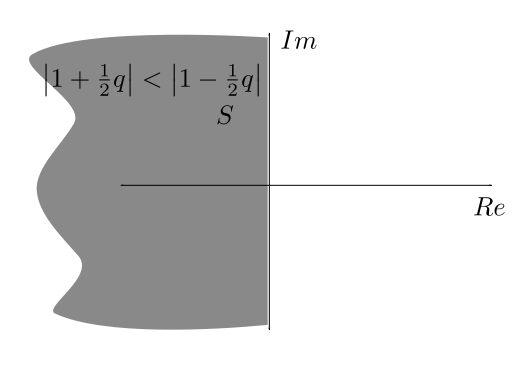
\includegraphics[width=\textwidth]{images/stability_trapez}
\caption{Das Stabilitätsgebiet des Trapez-Verfahrens. Insbesondere ist $|R(q)|=1$ wenn $q$ auf der komplexen Achse liegt, daher ist das Trapezverfahren A-stabil.}
\end{figure}

\end{bsp}

\subsubsection{Implizite Runge-Kutta-Verfahren}

Besonders gut geeignet für steife DGL

$$\Phi(t,h,y) = \sum_{i=1}^{r} \beta_i k_i $$

$$k_i = f(t+\gamma_i h,y +h \sum_{j=1}^{r} \alpha_{ij} k_j), i=1,\ldots,r$$

Butscher-Schema

\begin{table}[H]
\centering
\begin{tabular}{c| c c c c c}
$\gamma_1$ & $\alpha_{11}$ & $\alpha_{12}$ & $\ldots$ & $\ldots$ & $\alpha_{1r}$\\
$\gamma_2$ & $\alpha_{21}$ & $\alpha_{22}$ \\
$\gamma_3$ & $\alpha_{31}$ & $\alpha_{32}$ & $\alpha_{33}$\\
$\vdots$ & $\vdots$ & $\vdots$ & $\ddots$ & $\ddots$ \\
$\gamma_r$ & $\alpha_{r1}$ & $\alpha_{r1}$ & \ldots & $\alpha_{r,r-1}$ & $\alpha_{r,r}$ \\
\hline \\
 & $\beta_1$ & $\beta_1$ & \ldots & $\beta_{r-1}$ & $\beta_r$
\end{tabular}
\caption{Hier sind alle $\alpha_{ij}$ im Butscherschema nutzbar im Gegensatz zu Tabelle \ref{tab:ExplicitRkButscherScheme} auf Seite \pageref{tab:ExplicitRkButscherScheme}}
\end{table}




$\Rightarrow$ nichtlineares Gelichungssystem für die $k_i$

$$
\begin{pmatrix}
k_1 \\ \vdots \\ k_r
\end{pmatrix} = \begin{pmatrix}
f(t+\gamma_1 h, y + \sum_{j=1}^{r} \alpha_{ij} k_j) \\ \vdots \\ f(t+\gamma_1 h, y + \sum_{j=1}^{r} \alpha_{ij} k_j)
\end{pmatrix}
$$

Dadurch, dass ich mehr Paramter$\alpha_{ij}$ zur Verfügung habe $\Rightarrow$ bei impliziten r-stufingen RK-Verfahren kann man die Koeffizienten $\gamma_i, \beta_i, \alpha_{ij}$ so wählen, dass ein L-stabiles Verfahren der Ordnung $p=2r$ entsteht.





%===================================================== Vorlesung 03.06.2013
\subsection{Lösung nichtlinearer Gleichungssystem}

In der Praxis treten häufig nichtlineare Gleichungssystem auf

$$F(x)=0 ~ \text{mit}  ~  F: D \subset \mathbb{R}^{n} \rightarrow \mathbb{R}^{n}$$


\begin{bsp}[$y'=f(t,y)$]

$$y(t) \in \mathbb{R}^{n}$$ mit dem impliziten Eulerverfahren:

$$y_{k+1}=y_k + h f(t_{k+1},y_{k+1})$$

$$\Rightarrow x = y_{k+1}$$ löst das Gleichungssystem $F(x)=0$ mit
$$F(x)=x-y_k-h f(t_{k+1},x)$$
\end{bsp}


Gleichungssysteme hängen also eng mit \emph{Fixpunktgleichungen} zusammen

\begin{defi}[Fixpunktgleichung]
$$x=G(x)$$ mit $G: D\subset \mathbb{R}^{n} \rightarrow \mathbb{R}^{n} $ ist eine Fixpunktgleichung. $x^{*}$ heißt \emph{Fixpunkt} von $G$.

$$G \Leftrightarrow x^{*}=G(x^{*})$$
\end{defi}


\begin{bsp}[Fixpunkt impliziter Euler]

$$x=y_{k+1}$$ ist Fixpunkt von $$G(x)=y_k+hf(t_{k+1},x)$$
\end{bsp}

Zur Äquivalenz von Fixpunktgleichungen und Gleichungssystemen

\begin{description}
\item[$x=G(x)$] $\Leftrightarrow x-G(x)=0 \Leftrightarrow F(x)=0$ mit $F(x)=x-G(x)$
\item[$F(x)=0$] $\Leftrightarrow x=x-F(x) \Leftrightarrow x=G(x)$ mit $G(x)=x-F(x)$
\end{description}

Verallgemeinert:
Sei $M \in \mathbb{R}^{n \times n}$ invertierbar, dann
$$F(x)=0 \Leftrightarrow MF(x)=0 \Leftrightarrow x=G(x)$$ mit $G(x)=x-MF(x)$

$M$ spielt hier die Rolle eines \emph{Vorkonditionierers}.

\subsubsection{Fixpunktiteration und Fixpunktsatz von Banach}

Fixpunktiteration $x_0 \in D$ gegeben. Für $k=0,1,2,\ldots$ $$x_{k+1}=G(x_k)$$

Gesucht werden minimale Voraussetzungen an $G$, so dass $$x_k \stackrel{k\rightarrow \infty}{\rightarrow} x^{*}$$ und $$x^{*}=G(x^{*})$$


Bemerkung: Die \emph{Picard-Iteration} ist eine Fixpunkt-Iteration über Funktionen statt Vektoren.

\begin{figure}[H]
\includegraphics[width=\textwidth]{images/monotone_konvergenz}
\caption{Diese Bild zeigt \emph{monotone Konvergenz}, d.h wir nähern uns mit jeder Iteration dem Fixpunkt $x^{*}$ \emph{von einer Seite} an. Ausserdem wird hier und in den folgenden Abbildungen, der Vorgang der Fixpunktiteration graphisch dargestellt. Man beginnt mit einem Startwert $x_0$ und wertet diesen mit $G(x_0)$ aus. Dieses $G(x_0)$ ist mein erster Iterationsschritt $x_1$. Um die Position von $x_1$ graphisch zu bestimmen, nutzen wir die Gerade $y=x$. Dort wo sich die Funktionen $y=G(x)$ und $y=x$ schneiden, also an dem Punkt $G(x)=x$ befindet sich der Fixpunkt $x^{*}$}
\end{figure}

\begin{figure}[H]
\includegraphics[width=\textwidth]{images/nicht_monotone_konvergenz}
\caption{Auch hier konvergiert das Verfahren gegen den Fixpunkt $x^{*}$, allerdings nicht mehr von einer Seite. Die Iterationsschritte sind nun alterierend größer oder kleiner als der Fixpunkt.}
\end{figure}

\begin{figure}[H]
\includegraphics[width=\textwidth]{images/stetigkeit_fuer_fixpunkt}
\caption{Die Graphik veranschaulicht, dass Stetigkeit am Fixpunkt eine Voraussetzung für Konvergenz ist.}
\end{figure}

\begin{figure}[H]
\includegraphics[width=\textwidth]{images/keine_FP_konvergenz_01}
\caption{In diesem Fall konvergiert das Verfahren \emph{nicht}. Mit jedem Interationsschritt entfernen wir uns weiter vom Fixpunkt $x^{*}$. Der Grund hierfür ist die starke Steigung der Funktion, so dass für die Lipschitzkonstante $L$ gilt: $L>1$. Gleiches gilt auch für den Fall $L<-1$}
\end{figure}

\begin{figure}[H]
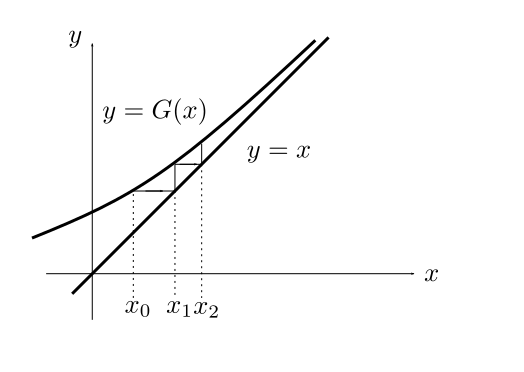
\includegraphics[width=\textwidth]{images/keine_FP_konvergenz_02}
\caption{ Auch bei \emph{asymptotischer Annäherung} der Funktion $y=G(x)$ an $y=x$ konvergiert das Verfahren \emph{nicht, obwohl} die Lipschitzkonstante die Bedingung $L<1$ erfüllt.}
\end{figure}

Anmerkung:
Besonders schenlle konvergenz hat man, wenn die Steigung von $G$ am Fixpunkt gleich Null ist. Dies heißt \emph{superlieare Konvergenz}.


Die obigen Abbildungen motvieren folgenden Satz

\begin{satz}[Fixpunktsatz von Banach]

Sei $D \subset \mathbb{R}^{n}$ abgeschlossen und $\not= 0$, und $G: D \rightarrow \mathbb{R}^{n}$ eine Abbildung mit folgenden Eigenschaften:

\begin{enumerate}
\item $G(D) \subseteq D$ d.h $\forall x \in D: G(x) \in D$ (Selbstabbildungseigenschaft)
\item G ist eine \emph{Kontraktion}, d.h. es gibt $0 < L < 1$ mit $$||G(x)-G(y)|| \leq L||x-y|| \forall x,y, \in D$$
\end{enumerate}

Dann gilt

\begin{enumerate}
\item Für jedes $x_0 \in D$ ist die Fixpunktiteration wohldefiniert und erzeugt die Folge $(x_r) \subset D$
\item $(x_r)$ konvergiert gegen ein $x^{*} \in D$
\item $x^{*}$ ist ein Fixpunkt: $x^{*} = G(x^{*})$
\item $x^{*}$ ist der einzige Fixpunkt von $G$ auf $D$
\item Fehlerabschätzung $$||x^{*}-x_k|| \leq \frac{L}{1-L}||x_k-x_{k+1}|| \leq \frac{L^{k}}{1-L}||x_1-x_0|| \forall k \geq 1$$
\end{enumerate}
\end{satz}


%============================================================= Vorlesung 04.06.2013

Bemerkung: Ist $\overline{x}$ ein Fixpunkt von $G$ und ist $G$ eine Kontraktion auf $D=K_r(\overline{x})=\{ x | ~ ||x-\overline{x}|| \leq r\}$, dann gilt $G(K_r(\overline{x})) \subset K_r(\overline{x})$

Denn:
$\forall x \in K_r (\overline{x}): ||G(x)-\overline{x}||=||G(x)-G(\overline{x})|| \leq L ||x-\overline{x}||\leq Lr < r$

Nachweise des Fixpunktsatzes von Banach:

\begin{enumerate}
\item Durchführbarkeit für bel. $x_0 \in D$ folgt aus $G(D) \subset D$
\item z.z: $x_r \rightarrow x^{*} \in D$ Hier steckt die Hauptarbeit: Für bel $k \geq 1:$ 

\begin{eqnarray*}
||x_{k+1}-x_k||&=&||G(x_k)-G(x_{k-1})|| \\
&\leq & L||x_k - x_{k-1}|| \\
&\leq & L^{2}||x_{k-1} - x_{k-2}|| \\
&\leq & \ldots \\
&\leq & L^{k}||x_{1} - x_{0}||
\end{eqnarray*}
Für beliebige $l > k$ folgt:
\begin{eqnarray*}
||x_l-x_k||&=&||(x_l-x_{l-1})+(x_{l-1}-x_{l-2})+\ldots \\
& & \ldots + (x_{k+2}-x_{k+1})+(x_{k+1}-x_k)|| \\
&\stackrel{\Delta-Ungl.}{\leq}& \sum_{j=k}^{l-1}||x_{j+1}-x_{j}|| \\
&\stackrel{s.o.}{\leq}& \sum_{j=k}^{l-1} L^{j} ||x_1 - x_0|| \\
&\leq & L^{k} ||x_1-x_0|| \sum_{i=0}^{\infty}L^{i} \\
&\stackrel{geom. Reihe}{=} & \frac{L^{k}}{1-L} ||x_1-x_0||
\end{eqnarray*}


Somit $||x_l-x_k|| \stackrel{l,r \rightarrow \infty}{\rightarrow} 0 \Rightarrow (x_k) $ ist eine \emph{Cauchy-Folge} und besitzt in $\mathbb{R}^{n}$ eine Grenzwert $x^{*}$. Mit $D$ abgeschlossen $D > (x_k) \rightarrow x^{*} \Rightarrow x^{*} \in D$
\item z.z: $$\underbrace{x_{k+1}}_{\rightarrow x^{*}}=\underbrace{G(\underbrace{x_k}_{\rightarrow x^{*}})}_{\rightarrow G(x^{*}), \text{da G stetig (Iteration)}} \blacksquare$$
\item z.z.: $x^{*}$ ist der einzige Fixpunkt in $D$. Annahme: $\overline{x} \in D, \overline{x} \not= x^{*}$ erfüllt ebenfalls $\overline{x}=G(\overline{x})$ Dann:
 $$||\overline{x}-x^{*}||=||G(\overline{x})-G(x^{*})|| \leq \underbrace{L}_{<1} ||\overline{x}-x^{*}|| < ||\overline{x}-x^{*}|| $$ Das ist aber ein Widerspruch! $\blacksquare$
\item Fehlerabschätzungen: $$||x_l-x_k|| \leq \frac{L^{k}}{1-L} ||x_1-x_0||, ~ \forall l>k$$ mit $l \rightarrow \infty$ nähert sich $x_l$ dem Fixpunkt $x^{*}$ an $$l \rightarrow \infty: ||x^{*}-x_k||\leq \frac{L^{k}}{1-L} ||x_1-x_0|| ,~ \forall k $$ speziell für $k=1$ gilt: $$ k=1: ||x^{*}-x_1|| \leq  \frac{L}{1-L} ||x_1-x_0||$$ Daher gilt allgemein: \begin{equation} \label{eqn:aposteriori} ||x^{*}-\underbrace{x_k}_{\text{ersetzt} ~ x_1}|| \leq \frac{L}{1-L} ||\underbrace{x_k}_{\text{ersetzt} ~ x_1} - \underbrace{x_{k-1}}_{\text{ersetzt} ~ x_0}|| \end{equation} Gleichung \ref{eqn:aposteriori} ist die \emph{aposteriori} Abschätzung (da ich die Abschätzung des Fehlers in Schritt $k$ auf dem Fehler im Schritt $k-1$ basiere, und dieser erst berechnet werden muss). Wir hatten $$||x_{k+1}-x_k|| \leq L^{k}||x_1-x_0||$$ mit einem \emph{Indexshift} in $k$
\begin{eqnarray*}
||x_k-x_{k-1}|| & \leq & L^{k-1} ||x_1-x_0|| \\
\Rightarrow  ||x^{*}-x_k|| &\leq & \frac{L}{1-L}||x_k-x_{k-1}|| \\
&\leq & \frac{L^{k}}{1-L} ||x_1-x_0||
\end{eqnarray*}


diese Abschätzung ist \emph{apriori} da ich mit dieser Fehlerbaschätzung schon nach einem Iterationschritt eine Oberschranke für den Fehler habe.
\end{enumerate}

Bemerkung: Die aposteriori-Abschätzung ist genauer als die apriori Abschätzung und kann als \emph{Abbbruchbedingung} verwendet werden.

Hilfsmittel zur Abschätzung von $L$:
Ist $D$ abgehschlossen und konvex, dann gilt: $$||G(x)-G(y)|| \leq L ||x-y||$$ mit $$L= \max\limits_{x \in D}  ||G'(x)||$$ wobei $$G'(x) \in \mathbb{R}^{n \times n} = \text{Jakobimatrix}$$ und Matrixnorm $$||M||=\max\limits_{||v||=1}||Mv||$$


Begründung: Setze $$\phi(t)=G(y+t(x-y))$$ Dann ist $$G(x)-G(y)=\phi(1)-\phi(0) = \int_{0}^{1} \phi'(t)dt = \int_{0}^{1}G'(y+t(x-y))(x-y)dt$$ und $$||G(x)-G(y)|| \leq \int_{0}^{1} \underbrace{||G'(\underbrace{y+t(x-y)}_{\in D})||}_{\leq L} \cdot ||x-y|| dt \leq L ||x-y||$$

Beobachtung: Ist $x^{*}=G(x^{*})$ und $||G'(x^{*})||<<1$. Dann, falls $G'$ stetig ist, folgt $||G'(x)||<<1$ in Umgebung von $x^{*} \Rightarrow$ sehr gute Kontraktion sobald die Fixpunktiteration in diese Umgebung eintritt.

Ideal (superlineare Konvergenz): $$||G'(x^{*})||=0$$


\begin{bsp}[Lipschitzkonstante und Fehler von $G(x)=\frac{x^{2}}{4}$]
$$G:\mathbb{R} \rightarrow \mathbb{R}, D=[0,1], G(x)=\frac{x^{2}}{4}$$

Dann: $G([0,1])=[0,\frac{1}{4}]\subset [0,1]$ d.h. Kontrkationsanforderung erfüllt

\begin{description}

\item[L-Konstante direkt abschätzen:] $$x,y \in [0,1]: |G(x)-G(y)|=\frac{1}{4}|x^{2}-y^{2}|=\underbrace{\frac{1}{4}|x+y|}_{\leq \frac{1}{2}=:L}|x-y|$$

\item[L-Konstante über Ableitung abschätzen:] $$x \in [0,1] \Rightarrow |G'(x)|=\left| \frac{x}{2} \right| \leq \frac{1}{2} =: L$$ (Anmerkung: Abschätzung über Ableitung üblicherweise schneller und einfacher!)

\item[Fehlerabschätzungen:] $$x_0=1 \Rightarrow x_1=G(x_0)=\frac{1}{4}$$

\begin{description}
\item[apriori] $$|\underbrace{x^{*}}_{=0}-x_k| \leq \frac{L^{k}}{1-L}|x_1-x_0| \stackrel{L=\frac{1}{2}}{=} \left( \frac{1}{2}\right)^{k-1} \cdot \frac{3}{4}$$
\item[aposteriori] $$|x^{*}-x_k| \leq \frac{L}{1-L}|x_k-x_{k-1}|\stackrel{L=\frac{1}{2}}{=}|x_k-x_{k-1}|$$
\end{description}

\end{description}

\end{bsp}

\begin{bsp}[Impliziter Euler als Fixpunktgleichung]



Anwendung auf impliziten Euler Schritt:

$$y'=f(t,y), ~ y(0)=y_0$$

Zeitschritt $y_j \rightarrow y_{j+1}$ mit impliziten Euler : $$y_{j+1}=\underbrace{y_j+hf(t_{j+1},y_{j+1})}_{=:G(y_{j+1})}$$


D.h $x=y_{j+1}$ ist Fixpunkt von $$G(x)=y_j+hf(t_{j+1},x)$$

Sei $L_f$ die Lipschitzkonstant von $f$ bzgl. $y$ d.h $$||f(t,y_1)-f(t,y_2)||\leq L_f ||y_1-y_2||$$

Dann 
\begin{eqnarray*}
||G(x_1)-G(x_2)||&=&h||f(t_{j+1},x_1)-f(t_{j+1},x_2)|| \\
& \leq & h L_f ||x_1-x_2||, ~ \forall x_1,x_2
\end{eqnarray*}

$\Rightarrow$ wir können $L=h L_f$ wählen. Mit $h < \frac{1}{L_f} \Rightarrow L < 1$

\end{bsp}

\begin{bsp}[Bestimme $L$ von $y'(t)=-99y(t)-\frac{y(t)}{1+y(t)^{2}}$]

$$y'(t)=-99y(t)-\frac{y(t)}{1+y(t)^{2}} , ~ y(0)=1$$

Suche das Ergebnis $y_1$ des ersten impliziten Eulerschritts, d.h $$y \approx y(\underbrace{t_1}_{=h})$$

Durch Anwenden des Fixpunktverfahrens. Hier $$f(t,y)=-99y-\frac{y}{1+y^{2}}$$

Bestimmung von $L_f$: 


\begin{eqnarray*}
|\partial_y f(t,y)| &=& |-99 + \overbrace{\frac{y^{2}-1}{(1+y^{2})^{2}}}^{|\cdot|\leq 1}| \\
&\overbrace{\leq}^{\text{scharf}(y=0)} & 100
\end{eqnarray*}


$\Rightarrow L_f = 100 \Rightarrow L = h L_f = 100h \Rightarrow h < \frac{1}{L_f}=\frac{1}{100}$

Nehmen wir zum Beispiel $h=\frac{1}{2 L_f}=0,005 \Rightarrow L=\frac{1}{2}$ und wählen $x_0=y_0=1$ dann

\begin{table}[H]
\centering
\begin{tabular}{c|l}
k & $|x_{k+1}-x_k|$ \\
\hline \\
0& 5.0 e-1\\
1& 2.5 e-1\\
2& 1.2 e-1\\
\vdots & \vdots \\
31& 1.8 e-10\\
32& 9.1e-11\\
\end{tabular}
\end{table}


\end{bsp}

Beobachtung: 
\begin{itemize}
\item Das Fixpunktverfahren ist universell
\item Konvergenz ist ernstahften Einschränkungen unterworfen
\item Konvergenzrate ist nur linear (Fehlerreduktion ca. um Faktor $L$ pro Iteration)
\end{itemize}

Wunsch: Schnelleres Verfahren $\rightarrow$ Newtonverfahren und Varianten


%=========================================================================== Vorlesung vom 10.6.2013 - von Assistentin gehalten

\subsubsection{Das Newtonverfahren für nicht-lineare Gleichungssysteme}

Nachteile der Fixpunktiteraton

\begin{itemize}
\item oft keine Kontraktion $\rightarrow$ Fixpunktverfahren konvergiert
\item langsame Konvergenz
\end{itemize}

$\Rightarrow$ Das Newtonverfahren ist Standard zur Nullstellensuche einer Funktion $F \in C^{1}$

\begin{defi}[Das Gauss-Newtonverfahren in $\mathbb{R}$]

\begin{eqnarray*}
x_{k+1} &=& x_k - \frac{F(x_k)}{F'(x_k)} \\
&& F \in C^{1} 
\end{eqnarray*}

\begin{figure}[H]

\includegraphics[width=\textwidth]{images/newton_verfahren}
\caption{Die Idee des \emph{Newtonverfahren} ist simpel. Man sucht den Punkt $F(x)=0$ welcher $x^{*}$ entspricht, indem am sich Schritt für Schritt mit den Nullstellen der linearen Approximation von $F'(x_k)$ an den jerweiligen $x_k$ an $x^{*}$ annähert. }
\label{fig:newtonverfahren}
\end{figure}

\end{defi}

\begin{bsp}[Anm. des Authors: Herleitung des Newtonverfahren]
Die Tangentengleichung an $x_k$ lautet, für eine Schrittweite $h$

$$t(x_k+h)=f(x_k)+F'(x_k)h$$

Nun setzten wir unsere Schrittweite $h=x-x_k$ und setzten in die Tangentengleichung ein

$$t(x)=F(x_k)+F'(x_k)(x-x_k)$$

Wir wählen nun $x_{k+1}$ so dass es die einzige Nullstelle dieser Tangente ist

\begin{eqnarray*}
t(x_{k+1})=F(x_k)+F'(x_k)(x_{k+1}-x_k) &\stackrel{!}{=}& 0 \\
\frac{F(x_k)}{F'(x_k)} + x_{k+1}-x_k &=& 0 \\
x_{k+1}  &=&  x_k -\frac{F(x_k)}{F'(x_k)}
\end{eqnarray*}

\end{bsp}

\begin{defi}[Das Gauss-Newtonverfahren im $\mathbb{R}^{n}$]


$$F(x)=0, F(x)=\begin{pmatrix}
F_1(x)  \\ F_2(x) \\ \vdots \\ F_n(x)
\end{pmatrix} \in \mathbb{R}^{n}
$$

Idee: In jedem Iterationsschritt wird $ F(x) $ durch eine lineare Approximation $ \tilde{F}(x)$ ersetzt und die Nullstelle von $ \tilde{F}(x)$ wird als Näherung für die Nullstelle $x^{*}$ interpretiert.

Linearisierung: $$F(x) = \underbrace{F(x_k) + F'(x_k)(x-x_k)}_{=: \tilde{F}_k(x)} + o(||x-x_k||)$$

$\rightarrow$ Newtonverfahren, falls $F'(x_k)^{-1}$ existiert: $$x_{k+1} = x_k - F'(x_k)^{-1}F(x_k)$$

\end{defi}

Die Bestimmung der Inversen $F'(x_k)^{-1}$ ist meist zu aufwändig. $\rightarrow$ bestimme Newton-Korrektur $s_k$ so dass

$$F'(x_k)s_k=-F(x_k)$$

und setzte $$x_{k+1}=x_k+s_k$$

Man kann das Newton-Verfahren als Fixpunktverfahren mit Iterationsfunktion (falls $F'(x)^{-1}$ existiert)

$$G(x)=x-F'(x)^{-1}F(x)$$
auffassen und kann Konvergenz-, Existenz und Eindeutigkeitsaussagen beweisen.

Alternativ: $$G_k(x):= x-\underbrace{F'(x_k)^{-1}}_{\text{Vorkonditionierung}}F(x)$$

Wir zeigen Konvergenz und Eindeutigkeit (Existenz setzten wir mal ohne Beweis voraus):

\begin{satz}[Lokale Konvergenz des Newton-Verfahrens]

$$\text{Sei} F:D \rightarrow \mathbb{R}^{n}$$ zwei mal stetig differenzierbra auf offener Menge $$D \subset \mathbb{R}$$ Weiter sei $x^{*}$ eine regläre Nullstelle von $F$ (d.h. $det(F'(x^{*})) \not= 0$, d.h. $F'(x^{*})$ regulär) Dann $\exists$ Umgebung von $x^{*}$

$$K_\rho (x^{*}) := \left\{  x \in \mathbb{R}^{n} : ||x-x^{*}|| \leq \rho \right\} \subset D$$

so dass für die Folge der Newton-Iterierten bei \emph{beliebigem} Startwert $x_0 \in  K_\rho(x^{*})$ gilt

$$x_k \in K_\rho(x^{*}) \forall k \geq 0, \lim\limits_{k \rightarrow \infty} x_k = x^{*}$$

$(x_k)$ konvergiert quadratisch gegen $x^{*}$ d.h. $\exists C > 0$:
$$ ||x_{k+1}-x^{*}|| \leq C ||x_{k}-x^{*}||^{2}$$ und $x^{*}$ ist die einzige Nullstelle von $F$ in $K_\rho(x^{*})$
\end{satz}


%==================================================== Vorlesung 11.06.2013 - von assistentin gehalten

\begin{bsp}[Beweis des lokalen Konvergenzsatzes des Newtonverfahrens]

Skizze:

Wir zeigen:
\begin{enumerate}
\item $\exists$ Umgebung $K_\rho (x^{*})$, in der $(F')^{-1}$ stetig/beschrängt ist
\item Für ein $x_k \in K_\rho(x^{*})$ definieren wir die Fixpunktiteration: $G_k(x):=x - F'(x_k)^{-1}F(x)$ und zeigen dass $G_k$ eine \emph{Kontraktion} auf $K_\rho(x^{*}) \forall k$ (mit 1 und Lipschitzstetigkeit von $F'$)
\item $x_{k+1} \stackrel{k \rightarrow \infty}{\rightarrow} x^{*} \forall x_0 \in K_\rho(x^{*})$ mit (2)
\item $x_{k+1} \stackrel{k \rightarrow \infty}{\rightarrow} x^{*}$ quadratisch (mit Taylorrestglied)
\item $x^{*}$ ist einzige Nullstelle von $F$ $\blacksquare$
 
\end{enumerate}

Erklärung für die schnelle Konvergenz des Newtonverfahrens:

Für $G(x):=x-F'(x)^{-1}F(x)$ gilt: $|G'(x)|=\ldots=\left| \frac{F''(x)F(x)}{(F'(x))^{2}}  \right| \leq C |F(x)|$ da $\frac{F''(x)}{(F'(x))^{2}}$ stetig ist in der Umgebung von $x^{*}$. Mit Taylor $ C |F(x)| = C|F(x)\underbrace{-F(x^{*})}_{\text{ =0, weil Nullstelle}}| \overbrace{=}^{Taylor} C|F'(x^{*}+t(x-x^{*}))(x-x^{*})| \underbrace{\leq}_{F' stetig} C \cdot L_F |x-x^{*}|$ für ein $t \in [0,1]$

$\Rightarrow |G(x)-x^{*}|=|G(x)-G(x^{*})| \leq |G'(x)||x-x^{*}| \leq C L_F |x-x^{*}||x-x^{*}| \Rightarrow$ die Kontraktionsrate wird kleiner, je näher man an der Nullstelle ist
\end{bsp}

\begin{bsp}[$y'(t)=-99y(t)-\frac{y(t)}{1+y(t)^{2}}$]

$$y(0)=1$$

Mit impl. Euler für $h=0,05 = \frac{5}{L_F}$ \begin{itemize}
\item Fixpunktitertaion divergiert
\item Newton braucht nur 3 Iterationen
\end{itemize}

Erklärung: $|G'(y_0)|<<1$ für $G(x)=x-\frac{F(x)}{F'(x)}$

\end{bsp}


Variationen des Newtonverfahrens:

\begin{defi}[Das vereinfachte Newtonverfahren]

$$F'(x_0)s_k=-F(x_k)$$
$$x_{k+1}=x_k+s_k$$

Bei dieser Variation des Newtonverfahrens wird immer das gleiche $F'(x)^{-1}$ benutzt, welches normalerweise $F'(x_0)^{-1}$ ist.

\begin{figure}[H]
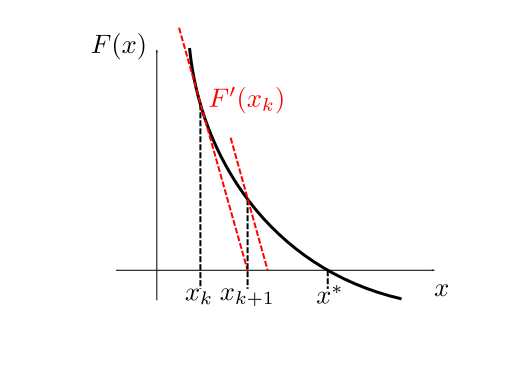
\includegraphics[width=\textwidth]{images/newton_verfahren_simplified}
\caption{Das verinfachte Gauss benutzt im vergelich zu herkömmlichen GNV nur die Steigung bei $x_0$. Dadurch entfällt die aufwändige berechnung/invertierung der Ableitung bei jedem neuen Iterationsschritt. Vergleiche Abbildung \ref{fig:newtonverfahren} auf Seite \pageref{fig:newtonverfahren}}
\end{figure}

Der Nachteil ist, dass es nur linear konvergiert, dafür ist es aber nicht so aufwändig.

\end{defi}

\begin{defi}[Das Sekantenverfahren]
$$x_{k+1}=x_k - \frac{x_k-x_{k-1}}{F(x_k)-F(x_{k-1})} F(x_k)$$

Das Sekantenverfahren ist eine Variation des Newtonverfahrens.

\begin{figure}[H]
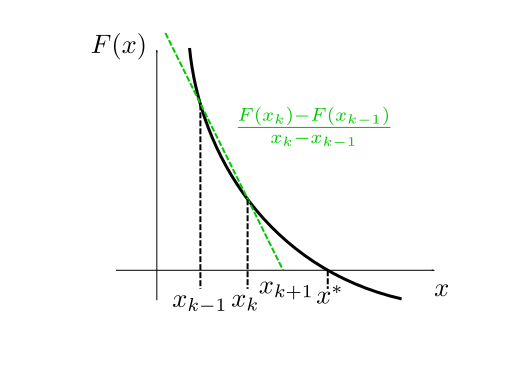
\includegraphics[width=\textwidth]{images/newton_verfahren_sekante}
\caption{Eine Variation des Newtonverfahrens, das nicht mit der Ableitung $F'(x)$ arbeitet, sondern die Sekante  benutzt}
\end{figure}

\end{defi}

\subsubsection{Ausgleichsprobleme}

Anwendung:
Bauteil mit unbekannter, nichtlinearer Kennlinie $k:[l,r] \rightarrow \mathbb{R}$

Zu Eingangsaten $u_1,....,u_m \in [l,r]$ stehen uns (fehlerbehaftete) Messungen zur Verfügung $b_1,...,b_m$ d.h $k(u_i)=b_i + \text{Fehler in der i-ten Messung}$

\begin{figure}[H]
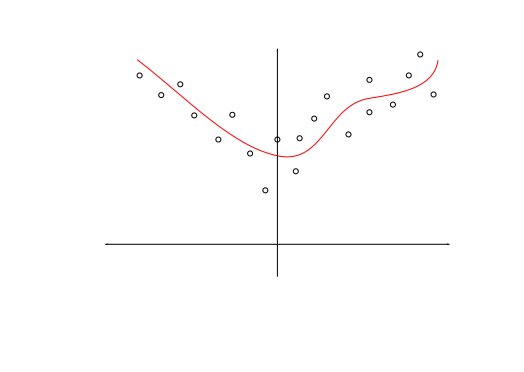
\includegraphics[width=\textwidth]{images/ausgleichsproblem}
\caption{Die Datenpunkte sind mit eine Fehler behaftet, und spiegeln daher nicht die Werte der exakten Funktion wieder.  Die "Rekonstruktion" der ursprünglichen Funktion aus den fehlerbehafteten Daten wird mittels Ausgleichrechnung gemacht.}
\end{figure}

Parametrischer Ansatz: z.B quadratisches Modell, d.h $$g(x,u)=x_1  +x_2u + x_3u^{2}$$

Interpoliere die Daten: $g(x,u_i)=b_i, \forall i=1,\ldots, m$

$$\underbrace{\begin{pmatrix}
1 & u_1 &u_1^{2} \\
1 & u_2 &u_2^{2} \\
\vdots & \vdots & \vdots \\
1 & u_m &u_m^{2} \\
\end{pmatrix}}_{=:A} \underbrace{\begin{pmatrix}
x_1 \\x_2 \\x_3 
\end{pmatrix}}_{=:x} = \underbrace{\begin{pmatrix}
b_1 \\b_2 \\ \vdots \\b_m
\end{pmatrix}}_{b}
$$

Falls $m>3$ ist das Gleichungssystem nicht lösbar $\rightarrow \min\limits_{x} ||A_x-b||$


Das ist ein lineares Ausgleichsproblem (kleinste Quadrate)

Alternativ statt Quadtratisch: $$g(x,u)=x_1u+x_2 e^{x_3 u}$$

Das ist ein nicht lineares Gleichungssytem $$F(x)=0, F_i(x)=x_1 u_i + x_2 e^{x_3 u_i} - b_i$$


$  \min\limits_{x} ||F(x)||_2$ Nichtlineares Ausgeleichsproblem/ kleinste Quadrate Problem.


Allgemein:

\begin{defi}[Lineares Ausgleichsproblem]

\begin{eqnarray*}
& & \min\limits_{x}  ||Ax-b||_2 \\
& \Leftrightarrow & \min\limits_{x} \frac{1}{2} ||Ax-b||^{2}_2 \\
& \Leftrightarrow & \min\limits_{x} \frac{1}{2} \sum_{i=1}^{m} (a_i^{T}x-b_i)^{2} \\
&& A \in  \mathbb{R}^{m \times n} \\
&& a_i = \text{i-te Zeile von A}\\
&& b \in  \mathbb{R}^{m} \\
&& m \geq  n
\end{eqnarray*}

Notwendige Optimierungsbedingungen

\begin{eqnarray*}
\nabla^{2} f(x)&=&A^{T}A \text{ ist positivsemidefinit} \\
&\Rightarrow & f \text{ konvex} \\
&\Rightarrow & \text{ hinreichend} 
\end{eqnarray*}

Hinreichende Optimierungsbedingung

\begin{eqnarray*}
\nabla f(x) &=& 0 \\
\Leftrightarrow A^{T}Ax&=&A^{T}b \text{(Normalengleichung)} 
\end{eqnarray*}

ist eindeutig lösbar, falls $$rang(A)=n$$

\end{defi}


\begin{defi}[Nchtlineares Ausgleichsproblem]

\begin{eqnarray*}
&&\min\limits_{x} ||F(x)||_2 \\
&\Leftrightarrow & \min\limits_{x} \frac{1}{2} ||F(x)||_2^{2}  \\
&\Leftrightarrow & \min\limits_{x} \frac{1}{2} \sum_{i=1}^{m} F_i(x)^{2}\\
&& F: \mathbb{R}^{n} \rightarrow \mathbb{R}^{n} \\
&& F \text{stetig differenzierbar}\\
&& m > n
\end{eqnarray*}

\end{defi}

\begin{bsp}[Standardverfahren zur Lösung mit Gauss-Newton-Verfahren]

Idee: Ersetze $F$ durch Linearisierung (in jedem Iterationsschritt)

\begin{eqnarray*}
F(x)&=&F(x_k)+F'(x_k)(x-x_k) + o(||x-x_k||_{2}) \\
& \rightarrow & \min\limits_x ||F(x_k)+F'(x_k)(x-x_k)||_2
\end{eqnarray*}



und das ist wieder ein lineares Ausgeleichsproblem, dass mit der  Normalengleichung gelöst werden kann (GNP = Gauss-Newton-Problem)

Löse GNP mit Normalengleichung: 

\begin{eqnarray*}
F'(x_k)^{T}F'(x_k)s_k&=&-F(x_k) \\
 \text{setzte } x_{k+1}&=&x_k+s_k
\end{eqnarray*}


\end{bsp}

\begin{bsp}[Gauss-Newton-Verfahren]

$$ $$

\begin{itemize}
	\item Vorgehen
	\begin{itemize}
		\item Wähle $x_0$ (möglichst nahe an Lösung $x^{*}$)
		\item Für $k=0, \ldots n$
		\begin{itemize} 
			\item löse $F'(x_k)^{T}F'(x_k)s_k=-F(x_k)$
			\item setzte $x_{k+1}=x_k+s_k$ 
			\item brich ab, falls $F'(x_k)^{T}F(x_k)$ klein genug.
		\end{itemize}
	\end{itemize}
	\item Eigenschaften und Voraussetzungen
	\begin{itemize}
		\item Das Gauss-Newton-Verfahren ist nur lokal konvergent
		\item Es konvergiert umso schneller je kleiner $||F(x^{*})||_2$ ist
		\item Voraussetzung (ähnlich wie bei Newton): $$F'(x^{*})^{T}F'(x^{*})$$ ist invertierbar
	\end{itemize}
	\end{itemize}
\end{bsp}


%================================================================================ Vorlesung 17.6.2013 -Prof Ulbrich himself

\begin{bsp}[Wiederholung Zusammenhang zwischen Newtonverfahren $F(x)=0$ und Fixpunktiteration]

Es gibt zwei Sichtweisen:
Newtonschritt: Wir sitzen in $x$ und machen den nächsten SChritt zu $$x^{+} = x \underbrace{- F'(x)^{-1}F(x)}_{\text{Newtonschritt s}}$$

Wenn ich nun $$x - F'(x)^{-1}F(x) =: G(x)$$ setze, habe ich damit gleich die Fixpunktgleichung $$x=G(x)$$

Wir stellen fest: Das Newtonverfahren ist die Fixpunktiteration für $$G(x)=x-F'(x)^{-1}F(x)$$

Man kann folgendes zeigen: $$F(\overline{x})=0 \Rightarrow G'(\overline{x})=0$$

\emph{Das Newtonverfahren konvergiert umso schneller, je näher wir an der Lösung sind.} Der Grund dafür ist die \emph{Vorkonditionierung} durch $F'(x)^{-1}$ die jedoch "teuer" zu berechnen sein kann.

D.h: Geben wir und ein beliebiges $L>0$ vor, dann gibt es $\epsilon > 0$ mit $||G'(x)|| \leq L \forall x$ mit $||x-\overline{x}|| \leq \epsilon$ $\Rightarrow$ Auf dieser Umgebung erzielen wir Kontraktionsrate $L$
\end{bsp}


\begin{bsp}[Wiederholung Ausgleichsproblemen]
Gegeben sei ein Modell, das den Ausgang einer Messung beschreibt und Parameter $x \in \mathbb{R}^{n}$ enthält:$M_i (x) \in \mathbb{R}$ ist der zur i-ten Messung gehörende Modelloutput, wenn die Modellparameter $x$ gewählt sind. $d_i \in \mathbb{R}$ sind die gemessenen Daten.

Ziel: Modelleichung, d.h. bestimme $x$ so, dass alle $M_i(x)$ möglichst gut mit $d_i(x)$ übereinstimmen. Was heisst möglichst gut übereinstimmen? Wir lösen $$\min\limits_{x \in \mathbb{R}^{n}} ||M(x)-d||$$ mit 

$$M(x)=\begin{pmatrix}
M_1(x)  \\ \vdots \\ M_n(x)
\end{pmatrix} ,
d=\begin{pmatrix}
d_1  \\ \vdots \\ d_n
\end{pmatrix}$$

Häufig sind die Messwerte ein Funktion von Systemparametern und Input $$M_i(x)=k(x,\underbrace{z_i}_{\text{Input}})$$

\begin{figure}[H]
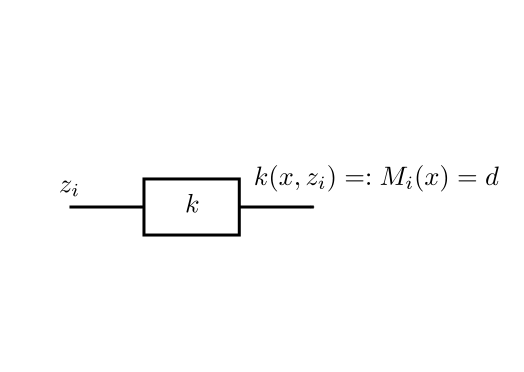
\includegraphics[width=\textwidth]{images/messvorgang}
\caption{Veranschaulichung eines Messvorgangs}
\end{figure}

Günstigere aufgeschrieben als KQ-Problem (KQ = kleinste Quadrate): $$\min\limits_{x} \frac{1}{2}||M(x)-d||^{2}$$ bzw $$\min\limits_{x} \underbrace{ \frac{1}{2}||F(x)||^{2}}_{=:f(x)}$$ mit $$M(x)-d=F(x)$$

Optimalitätsbedingung: $$\nabla f(x)=0$$

$$f(x)=\frac{1}{2} F(x)^{T}F(x) \Rightarrow \nabla f(x)=F'(x)^{T}F(x)$$


Lineare KQ-Probleme: $$F(x)=Ax-b \Rightarrow F'(x)=A \Rightarrow \nabla f(x)= A^{T}(Ax-b)$$

Somit: Lineares KQ-Problem:
$$\min\limits_{x} \underbrace{\frac{1}{2}||Ax-b||^{2}}_{f(x)}$$

In diesem Fall ist $f(x)$ konvex und quadratisch, d.h. 

\begin{eqnarray*}
\overline{x} &\text{löst}& \text{das Problem} \\
 \Leftrightarrow \nabla f(\overline{x})&=&0 \\
 \Leftrightarrow A^{T}A \overline{x}&=&A^{T}b \text{(Normalengleichung)}
\end{eqnarray*}

Im Fall eines nichtlinearen KQ-Problem kommt das Gauß-Newton-Verfahren zur Anwendung. Dieses erzeugt eine Folge $(x_k)$

Ist $x_k$ berechnet, so linearisiere $F$ um $x_k$ : $$F(x_k+s) \approx F(x_k) + F'(x_k)s$$ und berechne den Schritt $s_k$ durch ein lineares KQ-Problem $$\min\limits_{s \in \mathbb{R}^{n}} \frac{1}{2}||\underbrace{F(x_k)}_{=-b}+\underbrace{F'(x_k)}_{=A}s||^{2}$$ dies entspricht der Normalengleichung $$F'(x_k)^{T}F'(x_k)s_k = - F'(x_k)^{T}F(x_k)$$ und setze $$x_{k+1}=x_k+s_k$$
\end{bsp}

\subsection{Grundlagen zur Optimierung}
Optimierungsprobleme haben die Form: $$\min\limits_{x \in \mathbb{R}^{n}} f(x) \text{ unter Nebenbedingung } x \in X $$

$$f: \mathbb{R}^{n} \rightarrow \mathbb{R} \text{ Zielfunktion bzw. Kostenfunktion}$$

$$X \subset \mathbb{R}^{n} \text{ zulässiger Bereich}$$

Zahlreiche Anwendungen: KQ-Probleme, optimales Design (Schaltkreise, Materialien, Bauformen), optimale Steuerung(Robter, Motoren, Satellitenbahnen,$\ldots$)


Wiederholung: 
\begin{itemize}
\item $\overline{x}$ ist das lokale Minimum von $f$ auf $X$, falls es $\epsilon > 0$ gibt, mit $f(x) \geq f(\overline{x}) \forall x \in X, ||x-\overline{x}||<\epsilon$
\item $\overline{x}$ ist das globale Minimum von $f$ auf $X$ mit $f(x) \geq f(\overline{x}) \forall x \in X$
\end{itemize}


%================================================== Vorlesung 18.6.2013
Wir beschränken uns auf den unrestringierten Fall (d.h. ohne Nebenbedingung):
$$\min\limits_{x \in \mathbb{R}^{n}} f(x)$$

Mit der Voraussetzung dass $f$ stetig differenzierbar ist.

Wiederholung:

\begin{itemize}
\item Notwendige Optimalitätsbedingung erster Ordnung: $\overline{x} \in \mathbb{R}^{n}$ ist lokales Minimum von $f$ in $\mathbb{R}^{n}$ und $f $ ist $C^{1}$ dann gilt $$ \nabla f(\overline{x})=0$$ 
\item Notwendige Optimalitätsbedingung zweiter Ordnung: $\overline{x} \in \mathbb{R}^{n}$ ist lokales Minimum von $f$ in $\mathbb{R}^{n}$ und $f$ ist $C^{2}$, dann gilt $$\nabla f(\overline{x})=0$$ und $$\nabla^{2}f(\overline{x}) \text{ (=Hessematrix) ist positiv semi-definit}$$
\item Hinreichende Optimierungsbedingung zweiter Ordnung: Voraussetzung ist, dass $f C^{2}$ ist $\nabla f (\overline{x})$ und $\nabla^{2} f (\overline{x})$ positiv definit $\Rightarrow$ $\overline{x}$ ist lokales Minimum von $f$ (Hinreichende Bedinung ist \emph{keine} notwendige Bedingung)
\end{itemize}


\begin{defi}[Abstiegsrichtung]
Die Steigung von $f$ im Punkt $x \in \mathbb{R}^{n}$ in Richtung $s \in \mathbb{R}^{n} \backslash \{0\}$ ist definiert gemäß:
$$ \left. \frac{d}{dt} f(x+t \frac{s}{||s||}) \right|_{t=0} = \nabla f(x)^{T} \frac{s}{||s||} = \frac{\nabla f(x)^{T} s}{||s||}$$
$s$ heißt \emph{Abstiegsrichtung} von $f$ in Richtung $x$, falls die Steigung in Richtung $s<0$ ist, d.h. falls $\nabla f(x)^{T}s<0$
\end{defi}

Naheliegende Fragen:
Was ist das größte Gefälle von $f$ in $x$ und in welche Richtung tritt dies auf?

Abschätzung: $$|\text{Steigung entlang s}|= \left| \frac{\nabla f(x) s}{||s||} \right| \stackrel{Cauchy-Schwarz-Ungl.}{\leq} \frac{|| \nabla f(x)|| ||s||}{||s||} = ||\nabla f(x)||$$

Speziell:

$$s=\nabla f(x) \Rightarrow \text{Steigung entlang s} = \nabla f(x) = \frac{\nabla f(x)^{T} \overbrace{\nabla f(x)}^{=s} }{\underbrace{||\nabla f(x)||}_{||s||}} = \frac{||\nabla f(x)||^{2}}{||\nabla f(x)||}=||\nabla f(x)||$$

$$\Rightarrow s=\nabla f(x) \text{ist Richtung max. positiver Steigung}$$

$$\Rightarrow s=-\nabla f(x) \text{ist Richtung steilsten Abstiegs}$$


\begin{bsp}[Grundstruktur von Abstiegsverfahren]
$$ $$
\begin{enumerate}
\item In der aktuellen Iterierten $x_k \in \mathbb{R}^{n}$ wird eine Abstiegsrichtung $s_k$ bestimmt
\item Entlang dieser Richtung wird eine Liniensuche durchgeführt: Finde Schrittweite $\sigma_k>0$ mit $f(x_k+\sigma_k s_k)<f(x_k)$ und hinreichend guter f-Abnahmen
\item Neue Iterierte: $x_{k+1}:=x_k+\sigma_k s_k$
\item Wiederhole dieses Vorgehen
\end{enumerate}

\end{bsp}

Ziel: Wähle $s_k$ und $\sigma_k$ so, dass für jeden Häufungspunkt $\overline{x}$ von $(x_k)$ gilt: $\nabla f(\overline{x})=0$

Noch offen: Wie wählen wir die Suchrichtungen $s_k$?

\begin{itemize}
\item $s_k=-\nabla f(x_k)$=Richtung des Steilsten Abstiegs
\item $s_k=-\nabla^{2} f(x_k)^{-1} \nabla f(x_k)$ = Newton-Schritt
\end{itemize}

Wie wählen wir die Schrittweite $\sigma_k$? $\rightarrow$ Armijo-Schrittweitenregel.

\subsubsection{Schrittweitenregel}
Ziel:

\begin{itemize}
\item $f$-Abnahmen $f(x_k)-f(x_k+\sigma_k s_k)$ möglichst groß
\item Berechnung von $\sigma_k$ nicht zu aufwändig
\end{itemize}

Einige Möglichkeiten:

Sei $$\Phi_k(\sigma):=f(x_k+\sigma s_k)$$

\begin{description}
\item[Minimierungsregel:] Wähle $\sigma>0$ als Lösung von $\min\limits_{\sigma>0} \Phi_k(\sigma)$ (geht gut für quadratische $f$, für kubische $f$ oder größer zu aufwändig)
\item[erstes lokales Minimum:] $\sigma_k$ ist das erste lokale Minimum von $\Phi_k$ auf $(0,\infty) \rightarrow$ häufig ebenfalls zu aufwändig
\item[Armijo-Regel]: Ist die am häufigsten benutzte Regel. Bestimme das größte $\sigma_k \in \{ 1, \frac{1}{2}, \frac{1}{4}, \ldots \}$ für das gilt: $$f(x_k+\sigma_k s_k) \leq f(x_k) + \gamma \sigma_k \nabla f(x_k)^{T}s_k$$ mit $\gamma \in (0,1)$ fest (meist $\gamma \in [10^{-4},10^{-2}]$)
\end{description}


Interpretation der Armijo-Regel: $$ \text{Armijo-Regel } \Leftrightarrow \Phi_k(\sigma_k) \leq \Phi_k(0) + \gamma \Phi'_k(0)\sigma_k$$

\begin{figure}[H]
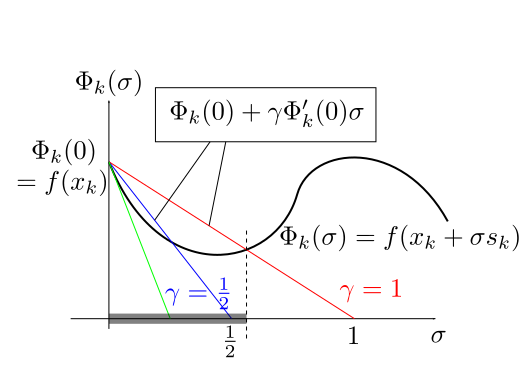
\includegraphics[width=\textwidth]{images/armijo}
\caption{Gesucht wird die größte Schrittweite $\sigma_k$ (im Bild $\sigma$) mit der die Armijo-Ungleichung noch erfüllt wird, d.h. die schwarze Funktion $\Phi_k(\sigma)$ ist kleiner als $\Phi_k(0)+\gamma \Phi_k'(0)\sigma$ Dazu probiert man nun mit dem Faktor $\gamma$ verschieden konfigurationen. Im Bild ist der Bereich, der die Armijo-Bedinung für $\gamma=1$ erfüllt, auf der $\sigma$-Achse grau markiert.}
\end{figure}

$\sigma_k$ Armijo-Schrittweite $\Rightarrow$ f-Abnahme bei Schrittweite $\sigma_k$ ist mindestens $\gamma \cdot \text{Gefälle}$ von $\Phi_k$ bei $\sigma=0 \cdot \text{Schrittweite} \sigma_k$

Das ist für Konvergenzbeweise und Praxis ausreichend.

\subsubsection{Berechnung von Abstiegsrichtungen, Winkelbedingungen}

Naheliegend und häufig verwendet: $s_k=-\nabla f(x_k)$. Das ist das \emph{Gradientenverfahren} bzw \emph{Das Verfahren des steilsten Abstiegs} (meist mit Armijo-Regel)

Beobachtung in der Praxis: Das Gradientenverfahren ist häufig sehr ineffizient.

Erklärung hierfür (sogar unter verwendung der besseren, aber aufändigeren Minimierungsregel für die Schrittweite):

$s_k=-\nabla f(x_k) =: -g_k$

Minimierungsregel $\Rightarrow \Phi'_k(\sigma_k)=0$, d.h. $\nabla f(\underbrace{x_k-\sigma_k g_k}_{x_{k+1}})^{T} \cdot \underbrace{(-g_k)}_{s_k}=-g_{k+1}^{T}g_k$ Der neue Gradient steht also \emph{senkrecht} zum alten Gradienten, daraus folgt, dass auch die neue Suchrichtung senkrecht zur alten Suchrichtung steht. Das ist unter Unmständen schlecht (Siehe CG-Verfahren in Wikipedia).


\begin{figure}[H]
\includegraphics[width=\textwidth]{images/cg_verfahren_wikipedia}
\caption{Hier sieht man, dass das Gradientenverfahren (grün) im Zick-Zack-Kurs gegen das Minimum konvergiert. Es ist offensichtlich, dass das CG-Verfahren (conjugated gradients) wesentlich schneller (in diesem Fall schon im zweiten Iterationsschritt!) konvergiert.}
\end{figure}

%================================================================================= Vorlesung 24.6.2013 - Prof himself

Beobachtung: Die Methode des steilsten Abstiegs $$s_k = -g_k = - \nabla f(x_k)$$ kann ein Zick-Zack-Verhalten aufweisen und ist daher häufig ineffizient. Wir benötigen "bessere" Suchrichtungen. Diese müssen zumindeste ein gewissens Mindestmaß an Abstieg aufweisen. Wie formulieren/quantifizieren wir das?

$s_k$ ist eine Abstiegsrichtung $\Leftrightarrow g_k^{T}s_k <0 \Leftrightarrow -g_ks_k > 0$

Steilstes Gefälle in $x_k$ ist $-||g_k||$ (erzielt durch $d=-g_k$)

Steigung entlang $s_k: $ $\frac{g_k^{T}s_k}{||s_k||}=\underbrace{\frac{-g_k^{T}s_k}{||s_k||||g_k||}}_{=: \rho(g_k, s_k)} \underbrace{(-||g_k||)}_{\text{steilstes Gefälle}}$

$\rho = $ ist nach dieser Formel ein Bruchteil bzw. Faktor des maximialen Gefälles, das entlang $s_k$ erzielt wird.

Interpretation von $\rho(g_k,s_k)$:
Man kann zeigen, dass $$\cos(\angle (v,w)) = \frac{v^{T}w}{||v||||w||}$$

 $$v=-g_k$$ $$w=s_k $$ $$\Rightarrow \rho(g_k,s_k)=cos\angle (-g_k,s_k)$$


Auf grund der letzten Gleichung heisst die Bedingung \emph{Winkelbedingung}.
\begin{figure}[H]
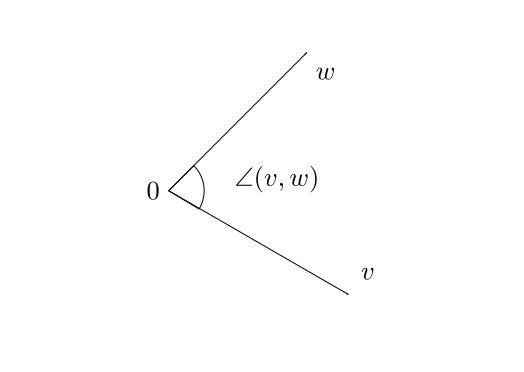
\includegraphics[width=\textwidth]{images/winkel}
\caption{Veranschaulichung zur Herleitung des Winkelsatzes}
\end{figure}





\begin{defi}[Winkelbedingung]
Wir fordern einen gewissen Mindestabstieg entlang $s_k$ durch folgende Winkelbedingung


\begin{equation}
\rho(g_k,s_k)\geq \eta 
\label{eqn:Winkelbedingung}
\end{equation}

mit $\eta \in (0,1)$ fest.

Interpretation: 

\begin{eqnarray*}
\rho &\geq& \eta \\
\Leftrightarrow cos(\angle (-g_k,s_k)) &\geq& \eta \\
\Leftrightarrow \angle(-g_k,s_k) &\leq & \alpha \in (0,\frac{\pi}{2})
\end{eqnarray*}
\end{defi}


\begin{defi}[Verallgemeinerte Winkelbedingung]

Man kann die Winkelbedingung $\rho \geq \eta$ verallgemeinern, indem man $\eta$ von $||g_k||$ abhängig macht. $$\rho(g_k,s_k) \geq \eta(||g_k||)$$ mit $\eta: \mathbb{R}_{+} \Rightarrow \mathbb{R}_{+}$ stetig, monoton wachsend mit $\eta(t)>0 ~ \forall t > 0$


\end{defi}

Wir benötigen noch eine letzte Zutat:

Da die \emph{Armijo-Regel} stets Schrittweiten $\leq 1$ liefert, gilt $||x_{k+1}-x_k|| \leq ||s_k||$ und wir müssen daher sicherstellen, dass $||s_k||$ nicht zu klein im Vergleich zu $||g_k||$ wird (Eine kleine Schrittweite bedeutet, dass viele Iterationsschritte zum erreichen des Ziels notwendig sind. Das wollen wir vermeiden)

Dies führt auf folgende Bedingung:

\begin{defi}[Längenbedingung an die Schrittweite]

\begin{equation}
||s_k|| \geq \kappa ||g_k||
\label{equ:Langenbedingung}
\end{equation}

mit Konstante $\kappa > 0$

Bemerkung: Auch hier kann (\ref{equ:Langenbedingung}) verallgemeinert werden mit $$\kappa \rightarrow \kappa(||g_k||)$$ $\kappa(t)$ muss die gleiche Bedingung wie $\eta(t)$ erfüllen

\end{defi}

Wie wir sehen werden, ist ein Abstiegsverfahren mit Armijo-Regel und Wahl der Suchrichtungen so dass Gleichung (\ref{equ:Langenbedingung}) und Winkelbedingung (\ref{eqn:Winkelbedingung}) erfüllt sind (bzw deren Verallgemeinerungen) golbal konvergent gegen Punkte mit $$\nabla f(\overline{x})=0$$

\begin{figure}[H]
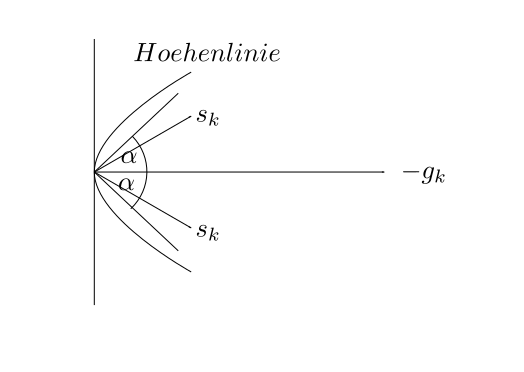
\includegraphics[width=\textwidth]{images/winkelbedingung}
\caption{Veranschaulichung zur Winkelbedingung. Im Prnzip verlange wir, dass sich der Winkel $\alpha$ zwischen 0 und $\frac{\pi}{2}$ befindet. Bei $\alpha=0$ gilt $s_k=-g_k$ wir gehen als in Richtung des steilsten Abstiegs. Im schlimmsten Fall ist $\alpha=\frac{\pi}{2}$ - dann bewegen wir uns im rechten Winkel zu $-g_k$ fort und bleiben gleich weit von der Lösung entfernt, wie zuvor.}
\end{figure}


Mögliche Wahl von geeigneten Suchrichtungen

\begin{itemize}
\item Richtung des steilsten Abstiegs
\item Newtonschritt
\item Newtonartige Schritte (z.B. BFGS)
\end{itemize}

Die verschiedenen Methoden werden nun etwas detailierter besprochen.

Richtung des steilsten Abstiegs  $$s_k = -g_k$$ hat bekanntlich Nachteile, aber

\begin{itemize}
\item es erfüllt Winkelbedingung (\ref{eqn:Winkelbedingung}) $\forall \eta \in (0,1]$
\item es erfüllt die Längebedingung (\ref{equ:Langenbedingung}) $\forall x \in (0,1]$
\end{itemize}



%========================================================================== Vorlesung  25.6.2013




Der Newtonschritt: $s_k$ löst TODO dann $\underbrace{\nabla^{2}f(x_k)}_{F'(x_k)}s_k=-\underbrace{\underbrace{\nabla f(x_k)}_{g_k}}_{F(x_k)}$ (= Newtonverfahren für $\underbrace{\nabla f(x)}_{=:F(x)}=0$)

Allerdings müssen wir prüfen, wann diese Methode die Winkelbedingung (\ref{eqn:Winkelbedingung}) und die Längebedingung (\ref{equ:Langenbedingung}) erfüllt.

Es sind zwei Voraussetzungen zu erfüllen 
\begin{enumerate}
\item $||\nabla^{2} f(x_k)|| \leq C ~ \forall k$
\item $0 < \lambda \leq \lambda_{\min} (\nabla^{2}f(x_k)) ~ \forall k$ 
\end{enumerate}



Aus den beiden Voraussetzungen folgen Winkelbedingung und Längenbedingung für geeignete Konstaten $\eta$ und $\kappa$: 

\begin{eqnarray}
||g_k||&=&||\nabla^{2} f(x_k) s_k|| \\
&\leq & ||\nabla^{2} f(x_k)|| \cdot ||s_k|| \\
&\stackrel{\text{Voraussetzung} 1}{\leq}& C ||s_k|| \\
\Rightarrow ||s_k|| &\geq & \frac{1}{C} ||g_k|| \\
\Rightarrow ||s_k|| &\geq & \kappa ||g_k||
\end{eqnarray}

 erfüllt falls $\kappa \leq \frac{1}{C}$

Zur Winkelbedingung (W)


\begin{eqnarray*}
-g_k^{T}s_k &\stackrel{Newton}{=}& s_k^{T}\nabla^{2}f(x_k)s_k \\
&\geq& \lambda_{\min} (\nabla^{2}f(x_k))||s_k||^{2} \\
&\geq& \lambda ||s_k||^{2} \\
\Rightarrow \rho(g_k,s_k)&=&\frac{-g_k^{T}s_k}{||g_k||||s_k||} \\
&\geq& \frac{\lambda ||s_k||^{2}}{||g_k||||s_k||} \\
&=& \lambda \frac{||s_k||}{||g_k||} \\
&\geq& \frac{\lambda}{C} \\
\Rightarrow \rho &>& \eta
\end{eqnarray*}

Diese Bedingung ist also erfüllt $\forall \eta \in (0,\frac{\lambda}{C}]$

Die beiden Bediungungen werden nicht immer erfüllt sein, d.h eine Absicherung/Prüfung ist nötig (dazu später)



Newtonartige Schritte:
Verwende statt $\nabla^{2}f(x_k)$ eine Approximation $$H_k = H_k^{T} \in \mathbb{R}^{n \times n} \Rightarrow H_k s_k = - \nabla f(x_k)$$

Besonders wichtiges Beispiel ist das \emph{BFGS-Verfahren}.

Beim BFGS-Verfahren wählt man eine symetrische, positiv definiete Startmatrix $H_k$ um so $s_0$ und daraus $x_1$ zu berechnen. In der $(k+1)$-ten Interatierten wird $H_{k+1}$ aus $H_k$ durch ein Rang-2-Update berechnet: $$H_{k+1}=H_k + \frac{y_k y_k^{T}}{y_k^{T} d_k} - \frac{(H_k d_k)(H_k d_k)^{T}}{d_k^{t}H_k d_k}$$ $$d_k = x_{k+1}-x_k$$ $$  y_k=g_{k+1}-g_k$$



$$\lambda_{\min} (M)= \min\limits_{v \not= 0} \frac{v^{T}Mv}{||v||^{2}}=\min\limits_{||v||=1} v^{T}Mv$$

$$M=UDU^{T}$$ mit $$U=(u_1,\ldots,u_n)$$ mit  $u_i$ Eigenvektor zum Eigenwert $\lambda_i$ $||u_i||=1$

$$D=\begin{pmatrix}
\lambda_1 & & 0\\ & \ddots & \\ 0 & & \lambda_n
\end{pmatrix}$$


mit $$\lambda_{\min}(M)= \lambda_1 \leq \ldots \leq \lambda_n$$ 


\subsubsection{Ein globaler Konvergenzsatz}

\begin{bsp}[Abstiegsverfahren mit Arminjo-Regel]

$$ $$
\begin{enumerate}
\item Wähle Startpunkt $x_0 \in \mathbb{R}^{n}, \epsilon \geq 0$ für $k=0,1,2, \ldots$
\item Stop, falls $||g_k|| \leq ||\epsilon||$
\item Berechne eine Suchrichtung $s_k$, welche die Winkelbedingung und Längenbedingung erfüllt (durch $s_k=-g_k$ oder $s_k$ ist Newtonschritt mit BFGS-Regel)
\item Berechne die Schrittweite $\sigma_k$ durch die Armijo-Regel
\item Setze $x_{k+1}:= x_k + \sigma_k s_k$
\end{enumerate}

\end{bsp}


\begin{satz}[Globale Konvergenz]


Sei $$f C^{1}$$ und $$\epsilon=0$$. Dann 

\begin{itemize}
\item gibt es entweder ein $k$ mit $\overbrace{\nabla f(x_k)}^{g_k}=0$ oder
\item das Abstiegsverfahren erzeugt eine Folge $(x_k)$, deren Häufingspunkte $\overline{x}$ die Optimalitätspedingung $\nabla f(\overline{x})=0$ erfüllen
\end{itemize}

\end{satz}

% 2.3.4
\subsubsection{Globalisiertes Newton-Verfahren}
Hier wird $s_k$=Newton-Schritt gewählt, wann immer möglich (Winkelbedingung muss erfüllt sein) Andernfalls wird auf $s_k=-g_k$ ausgerichtet.



\begin{bsp}[Globalisiertes Newton-Verfahren]

$$ $$

\begin{enumerate}
\item Wähle $x_0 \in \mathbb{R}^{n}, \epsilon > 0 , 0 < \eta_1 , \eta_2 < 1, \beta>0$

für $k=0,1,\ldots$

\item Berechne $g_k := \nabla f(x_k)$

\item Stop falls $g_k =0$
\item Falls möglich, berechne den Newton-Schritt $d_k$ durch $$\nabla^{2} f(x_k) d_k = -g_k$$

Ist $d_k$ berechenbar und gilt die verallgemeinerte Winkelbedingung $\rho(g_k,d_k) \geq \underbrace{\min(\eta_1,\eta_2 ||g_k||^{\beta})}_{\eta(||g_k||)}$  so setze $s_k=d_k$, sonst setzte $s_k=-g_k$

\item Berechen Schrittweite $\sigma_k$ mit Arminjo-Regel

\item Setzte $x_{k+1}:=x_k+\sigma_k s_k$
\end{enumerate}


\end{bsp}

\begin{satz}[Konvergenz des globalisierten Newtonverfahren]
Das globalisierte Newtonverfahren konvergiert im Sinnes des vorherigen Konvergenzsatzes. Ist $\gamma < \frac{1}{2}$ in der Armijo-Regel und $\overline{x}$ ein Häufungspunkt von $(x_k)$ mit $\lambda_{\min} (\nabla^{2}f(\overline{x})) \geq \lambda > 0$, dann geht das Verfahren irgendwann in das ungedämpfte ($\sigma_k=1$) Newtonverfahren über $\Rightarrow$ schnelle lokale Konvergenz
\end{satz}


\subsubsection{Globalisierung des Newtonverfahrens für Gleichungssysteme}
Für das System $F(x)=0$ verwenden wir zur Globalisierung die Winkelbedingung und die Armijo-Regel für die Zielfunktion $f(x)=\frac{1}{2}||F(x)||^{2}$($\Rightarrow \nabla f(x)=F'(x)^{T}F(x)$)



Vorgehen wie im globalen Newton-Verfahren für Minimierungsprobleme, allerdings mit $d_k$ aus $F'(x_k) d_k = -F(x_k)$ Alles andere bleibt unverändert und verwendet $f(x)=\frac{1}{2} ||F(x)||^{2}, \nabla f(x)=F'(x)^{T}F(x)$

\section{Komplexe Funktionen}
Wir beschäftigen uns hier mit den Eigenschaften von Funktionen

$$f: U \subset \mathbb{C} \rightarrow \mathbb{C}$$ mit $U \subset \mathbb{C}$ offen

\begin{defi}[Komplexe Exponentialfunktion]
$$e^{z}:=e^{x+iy}=e^{x}e^{iy}$$ $$x=Re(z),$$ $$y=Im(z), $$ $$z=x+iy$$ wobei $$e^{iy}=\cos y + i \sin y$$
Reihendarstellung $$e^{z}=\sum\limits_{k=0}^{\infty} \frac{z^{k}}{k!}$$ konvergiert auf ganz$ \mathbb{C}$
\end{defi}

\begin{defi}[Komplexer Kosinus und Sinus]
$$\cos z = \frac{1}{2} (e^{iz}+e^{-iz})=\sum\limits_{k=0}^{\infty}(-1)^{k} \frac{z^{2k}}{(2k)!}$$
$$\sin z = \frac{1}{2i} (e^{iz}-e^{-iz})=\sum\limits_{k=0}^{\infty}(-1)^{k} \frac{z^{2k+1}}{(2k+1)!}$$
\end{defi}

%========================================================= Vorlesung vom 01.07.2013 - gehalten von Dominik Meidber (Oberassistent)

\subsection{Potenzreihen in $\mathbb{C}$}


Potenzreihe $$f(z)=\sum_{k=0}^{\infty} a_k (z-z_0)^{k} , a_k \in \mathbb{C}, z_0 \in \mathbb{C}$$


\begin{satz}[Konvergenz von Folgen in $\mathbb{C}$]

Eine Potenzreihe heißt an der Stelle $z \in \mathbb{C}$ konvergent, wenn die Folge der Partialsummen $$s_n=\sum_{k=0}^{n}a_k (z-z_0)^{k}$$

für $n\rightarrow \infty$ in $\mathbb{C}$ konvergiert.

\end{satz}

Aus Mathe 1 und 2 wissen wir: Für eine Potenzreihe $\sum_{k=0}^{\infty}a_k(z-z_0)^{k}$ gelten folgende Aussagen:

Es gibt einen $R \in (0, \infty]$ (Konvergenzradius) mit

\begin{itemize}
\item $R=0 \rightarrow$ Reihe konvergerit für $z=z_0$
\item $R \in (0,\infty) \rightarrow$ Reihe konvergiert für $z$ mit $|z-z_0|<R$ absolut und divergiert für alle für $z$ mit $R<|z-z_0|$
\item $R = \infty \rightarrow$ Reihe konvergeirt für alle $z \in \mathbb{C}$
\item Es gilt $R=\frac{1}{\limsup\limits_{k \rightarrow \infty} \sqrt[k]{|a_k|} }$
\item Es gilt $R=\lim\limits_{k \rightarrow \infty} \frac{|a_k|}{|a_{k+1}|}$ falls dieser Grenzwert exisitert
\end{itemize}

\subsection{Komplexe Differenzierbarkeit}

\begin{defi}[Komplexe Differenzierbarkeit]

$$f: U \rightarrow \mathbb{C} , U \subset \mathbb{C} \text{ offen}$$ heißt komplex differenzierbar in $z \in U$, falls der folgende Grenzwert exisitiert $$f'(z) := \lim\liminf_{h \in  \mathbb{C}, h \rightarrow 0} \frac{f(z+h)-f(z)}{h}$$

$f'(z)$ heisst Ableitung von $f$ an der Stelle $z$

Ist $f$ in jedem Punkt $z \in U$ differenzierbar, dann heißt $f$ \emph{analytisch bzw. holomorph}
\end{defi}

Bemerkung: Ist $f$ in $z$ komplex differenzierbar, dann folgt:

$$\frac{f(z+h)-f(z)-f'(z)h}{h}=\frac{f(z+h)-f(z)}{h}-f'(z) \rightarrow 0$$

$$\Rightarrow |f(z+h)-f(z)-f'(z)h|=o(|h|)$$


\begin{satz}[Regeln für komplexes Differenzieren]
Für komplex differenzierbare Funktionen gelten die Summen-, Produkt-, Quotienten- und Kettenregeln.
\end{satz}


\begin{bsp}[Zeige $\left( \frac{1}{z} \right)' = -\frac{1}{z^{2}}$]

$$\left( \frac{1}{z} \right) = -\frac{1}{z^{2}}$$

$$\frac{\frac{1}{z+h}-\frac{1}{z}}{h} = \frac{\frac{z-(z+h)}{(z+h)z}}{h}=-\frac{1}{(z+h)z} \stackrel{h \rightarrow 0}{\rightarrow} - \frac{1}{z^{2}}$$
\end{bsp}

\begin{bsp}[Zeige $(z^{n})'=n \cdot z^{n-1}$]
Durch Induktion:
TODO
\end{bsp}

\begin{bsp}[Komplexe Differenzierbarkeit von $f(z)=\overline{z}$]
$$f(z)=\overline{z}$$

$$\frac{\overline{z+h} - \overline{z}}{h} = \frac{\overline{h}}{h}$$

Betrachte zwei Nullfolgen $h\rightarrow 0$ in $\mathbb{C}$

$h=it, t \in \mathbb{R}, t\rightarrow 0$

$$\frac{\overline{h}}{h}=\frac{-it}{it}=-1$$

$h=t \in \mathbb{R}$

$$\frac{\overline{h}}{h} = \frac{t}{t} = 1$$

$$ \Rightarrow \frac{\overline{h}}{h} \text{existiert nicht}$$

D.h. $f(z)=\overline{z}$ ist \emph{nicht} komplex differenzierbar

\end{bsp}

\begin{bsp}[Komplexe Differenzierbarkeit von $f(z)=Re(z)$]
$$f(z)=Re(z)=\frac{1}{2}(z+\overline{z})$$ ist auch nicht komplex differnzierbar (siehe vorheriges Beispiel)
\end{bsp}


\begin{satz}[Konvergenzradius differenzierbarer Funktionen]

$$ $$
Sei $$f(z)=\sum_{k=0}^{\infty} a_k (z-z_0)^{k}$$ mit Konvergenzradius $R \in (0,\infty]$ Dann ist $f$ auf $B_R(z_0)$ komplex differenzierbar mit 
$$f'(z)=\sum_{k=1}^{\infty} k a_k (z-z_0)^{k-1}$$

Die Reihe für $f'$ besitzt wider den Konvergenzradius $R$

$$\stackrel{\text{Indutkiv}}{\Rightarrow} f^{(n)}(z)=\sum_{k=n}^{\infty} (k-n+1) \ldots  k a_k (z-z_0)^{k-n}$$ 
$$ \Rightarrow a_k =\frac{f^{(k)}(z_0)}{k!} , \forall k \geq 0$$
\end{satz}

%=================================================== Vorelesung 02.07.2013

Teilwwiser Nachweis des Satzes: Formell duch summenweises Differenzieren (erfordert Konvergenz d. $f(z)$-Reihe und gleichmäßige Konvergenz der $f'(z)$-Reihe)

Konvergenz-Radius der $f'$-Reihe im Fall, dass $\lim\limits_{k \rightarrow \infty} \left| \frac{a_k}{a_{k+1}}\right| = R$ existiert. Dann: Konvergenzradius von $f'$-Reihe
$$\lim\limits_{k \rightarrow \infty} \left| \frac{b_{k-1}}{b_k}\right|=\lim\limits_{k \rightarrow \infty} \left| \frac{k a_{k}}{(k+1)a_{k+1}}\right| = 
\lim \underbrace{\frac{k}{k+1}}_{\rightarrow 1} \underbrace{\left| \frac{ a_{k}}{a_{k+1}}\right|}_{\rightarrow R} =R$$

Formel für $a_n$: $f^{(n)}(z)=1 \ldots n a_n (z-z_0)^{0} + 2 \ldots (n+1)a_{n+1}(z-_0)^{1}+ \ldots \Rightarrow f^{(n)}(z_0)=\underbrace{1 \ldots n}_{n!} a_n \cdot 1 = n! \cdot a_n$ 


\begin{bsp}[Ableiten von $f(z)=\frac{1}{1-z}$]

$$f(z)=\frac{1}{1-z}=\sum_{k=0}^{\infty} z^{k}$$ $$R=1$$ $$z_0=0$$

Direktes Ableiten von $f(z)$

$$f'(z)=\frac{1}{(1-z)^{2}}, (|z|<1)$$

Ableiten der Reihe

$$f'(z)=\sum_{k=1}^{\infty} k z^{k-1}, (|z|<1)$$

$$\Rightarrow f'(z)=\frac{1}{(1-z)^{2}}=\sum_{k=1}^{\infty} k z^{k-1}, (|z|<1)$$


\end{bsp}


\begin{bsp}[Ableiten von $f(z)=e^{z}$]

$$f(z)=e^{z}=\sum_{k=0}^{\infty} \frac{z^{k}}{k!}, R=\infty, z_0=0$$

Ableiten der Reihe:

$$f'(z)=\sum_{k=1}^{\infty} \frac{k}{k!}z^{k-1}=\sum_{k=1}^{\infty} \frac{1}{(k-1)!} z^{k-1}=\sum_{k=0}^{\infty} \frac{z^{k}}{k!}=e^{z}$$


\end{bsp}

\subsubsection{Zusammenhang mit der reellen Differenzierbarkeit}

Wir indentifizieren eine Funktion $$f: U \subset \mathbb{C} \rightarrow \mathbb{C}$$ mit einer Funktion $$ \tilde{f}: \tilde{U} \subset\mathbb{R}^{2} \rightarrow \mathbb{R}^{2}$$

$$z \in U, z=x+iy \hat{=} \begin{pmatrix}
x \\y
\end{pmatrix} \in \tilde{U} \subset \mathbb{R}^{2}
$$

$$f(x+iy)=u(x,y)+iv(x,y)\hat{=} \tilde{f}(x,y)=\begin{pmatrix}
u(x,y)\\v(x,y)
\end{pmatrix} \in \mathbb{R}^{2}$$

Sei $f$ in $z$ komplex differenzierbar.

Wir schreiben $f'(z)=a+ib, h=s+it \hat{=} \begin{pmatrix}
s\\t
\end{pmatrix}  $ Dann

$f'(z)h=(a+ib)(s+it)=(as-bt)+i(at+bs)\hat{=}\begin{pmatrix}
as-bt \\at+bs
\end{pmatrix} = \begin{pmatrix}
a & -b \\ b& a
\end{pmatrix}  \begin{pmatrix}
s \\t
\end{pmatrix} $

Nun: $|f(z+h)-f(z)-f(z)h|=o(|h|) \hat{=} ||\tilde{f}(x+s,y+t)-\tilde{f}(x,y)- \begin{pmatrix}
a & -b \\ b& a
\end{pmatrix}  \begin{pmatrix}
s \\t
\end{pmatrix} || = o(|| \begin{pmatrix}
s\\t
\end{pmatrix} ||)$


$\Rightarrow \tilde{f}$ ist reell differenzierbar in $(x,y)$ mit $$\tilde{f}'(x,y)= \begin{pmatrix}
u_x(x,y) & u_y(x,y)\\
v_x(x,y) & v_y(x,y)
\end{pmatrix} = \begin{pmatrix}
a & -b \\ b & a
\end{pmatrix} $$

wobei $$a=Re(f'(x+iy))$$ $$b=Im(f'(x+iy))$$

$\Rightarrow \tilde{f}= \begin{pmatrix}
u \\ v
\end{pmatrix} $ hat eine Jakobimatrix mit besonderer Struktur.


Wir folgern: Ist $f(\underbrace{x+iy}_{z})= u(x,y)+iv(x,y)$ komplex differenzierbar, dann gelten die \emph{Cauchy-Riemann-Differenzialgleichungen}

\begin{defi}[Cauchy-Riemann-Differenzialgleichungen]

$$u_x(x,y)=v_y(x,y)$$

$$u_y(x,y)=-v_x(x,y)$$

\end{defi}

\begin{satz}[Komplexe Differenzierbarkeit] 


$$f: U \subset \mathbb{C} \rightarrow \mathbb{C} , f(x+iy)=u(x,y)+iv(x,y)$$ ist komplex differenzierbar in $x+iy$ genau dann, wenn $\tilde{f}(x,y)= \begin{pmatrix}
u(x,y) \\v(x,y)
\end{pmatrix} $ in $ \begin{pmatrix}
x \\ y
\end{pmatrix} $ differenzierbar und die Cauchy-Riemann-DGL'n gelten.

Es gilt die Formel

$$f'(x+iy)=\underbrace{u_x(x,y)}_{=a}-i\underbrace{u_y(x,y)}_{=-b}=\underbrace{v_y (x,y)}_{=a} + i\underbrace{v_x(x,y)}_{=b}$$


\end{satz}


\begin{bsp}[Komplexe Diff'barkeit von $f(z)=\overline{z}$ mit CR prüfen]

$$f(z)=\overline{z}=x-iy$$

$$\Rightarrow u(x,y)=x, v(x,y)=-y$$

$$\Rightarrow u_x=1 \not= -1 = v_y$$

Das verletzt die erste CR-Gleichung

$\Rightarrow z \rightarrow \overline{z}$ ist nicht komplex differenzierbar.


\end{bsp}


\begin{bsp}[Komplexe Diff'barkeit von $f(z)=Re(z)$ mit CR prüfen]

$$f(z)=Re(z)$$

$$u=x$$
$$v=0$$

$$u_x=1 \not= 0 = v_y$$

Das verletzt die erste CR-Gleichung

$f(z)=Re(z)$ ist nicht komplex differenzierbar.

\end{bsp}


\begin{satz}[Eigenschaften analytischer Funktionen]
$f,g$ analytisch ($\hat{=}$ komplex differenzierbar) auf $U$ mit $f=g'=0$, dann folgt $f=g+const.$ 

TODO: Interpretation

\end{satz}

\begin{satz}[Eigenschaften analytischer Funktionen]
Ist $f:U \rightarrow \mathbb{C}$ analytisch auf $U$ mit $|f| \equiv const$, dann folgt $f \equiv const.$ auf $U$

Nachweis:

$$|f| \equiv 0 \Rightarrow f \equiv 0$$


$$|f| \equiv C \not= 0 \text{ auf } U \Rightarrow f(z) \not= 0 \forall z \in U $$ und 
$$ f(z) \overline{f(z)}=|f(z)|^{2}=C^{2}$$

Also

$$\overline{f(z)}=\frac{C^{2}}{f(z)}$$ komplex differentierbar auf $U$, da dies für $f(z)$ gilt.

$$f(z)=u+iv$$

$$\Rightarrow u_x=v_y, u_y=-v_x$$

$$\overline{f(z)}=u-iv = \hat{u}+i\hat{v}$$

$$\Rightarrow \hat{u}_x=\hat{v}_y, \hat{u}_y=-\hat{v}_x$$

$$\Rightarrow v_y=u_x=-v_y \Rightarrow v_y=0 \Rightarrow u_x=0$$

$$\Rightarrow -v_x=u_y=v_x \Rightarrow v_x=0 \Rightarrow u_y=0$$

$\Rightarrow u, v$ sind konstante Funktionen, d.h.$f$ ist konstant

TODO: Interpretation

\end{satz}


Interpretation der Ableitung als Drehstreckung:
Polardarstellung

$$f'(z)=|f'(z)| e^{i \Phi}, h=h|h|e^{i \alpha} \Rightarrow f'(z)h=|f'(z)||h|e^{i(\alpha + \Phi)}$$

\begin{figure}[H]
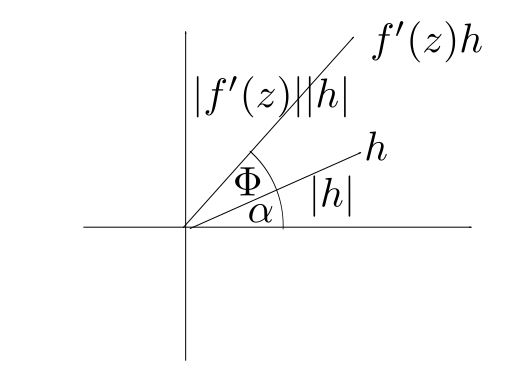
\includegraphics[width=\textwidth]{images/complex_multi}
\caption{Eine Drehstreckung von $h$ durch $f'$. Das entspricht einer Multiplikation in $\mathbb{C}$}
\end{figure}

\begin{satz}[Konformität von analytischen Funktionen]
$$ $$
Jede analytische Funktion mit $f'(z)\not=0$ auf $U$ ist konform, d.h. \emph{winkel- und orientierungstreu}.

Begründung:

Schneiden sich zwei $C^{-1}$-Kurven $w(t) \in \mathbb{C}$ und $k(t) \in \mathbb{C}$ im Punkt $\hat{z}=w(t_1)=k(t_2)$, dann haben sie dort die Tangenten $w'(t_1)$ bzw $k'(t_2)$

Die Tangenten der Bildkruven $f(w(t))$ bzw $f(k(t))$ im Punkt $f(\hat{z})$ sind gegeben durch $\underbrace{f'(w(t_1))}_{f'(\hat{z})}w'(t_1)$ bzw $\underbrace{f'(k(t_2))}_{f'(\hat{z})}k'(t_2)$

D.h. beide Tangeten werden um den gleichen Winkel gedreht und um den gleichen Faktor gestreckt.

\begin{figure}[H]
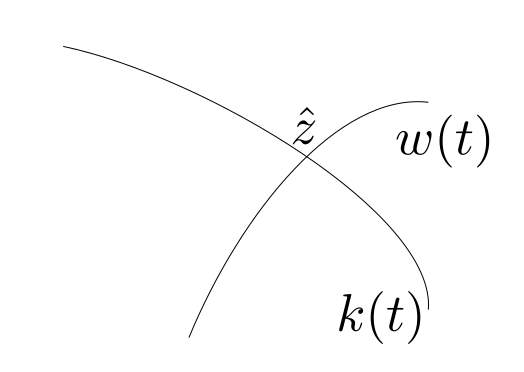
\includegraphics[width=\textwidth]{images/winkeltreue}
\caption{Die zwei Kurven $w$ und $k$. Unter einer Abbildung (z.B. einer Mulitplikation mit $e^{i\Phi}$ was einer Drehung entspricht) bleibt der Winkel zwischen den Tangenten $w'$ und $k'$ im Punkt $\hat{z}$ erhalten.}
\end{figure}

\end{satz}

Folgerung: Die Koordinatenlinien $x \equiv const.$ und $y \equiv const.$ sind orthogonal zueinander in der $z=x+iy$-Ebene werden durch die holomorphe Abbildung $f=u+iv$ auf zueinander orthogonale Bildkruven abgebildet.



%========================================================================================================== Vorlesung 8.7.2013

\subsection{Komplexe Kurvenintegrale}

Für $v: [a,b] \rightarrow \mathbb{C}$ stetig, $v(t)=v_1(t) + iv_2(t)$ definieren wir


$$\int_{a}^{b}v(t) dt := \int_{a}^{b} v_1 (t) dt + i \int_{a}^{b} v_2(t) dt$$

\begin{defi}[Aufteilung in Teilkurven]
$$f: U \subset \mathbb{C} \rightarrow \mathbb{C}$$ sei stetig, $U$ offen. Weiter sei $w:[a,b] \rightarrow U$

Dann ist das Integral von $f$ entlang $w$ definiert durch $$ \int_{w} f(z) dz := \int_{a}^{b} f(w(t))w'(t) dt$$

Besteht $w$ aus endlich vielen stetig differenzierbaren Teilkurven $$w_k:[a_k,b_k] \rightarrow U$$ dann definieren wir $$\int_{w} f(z) dz := \sum_{k=1}^{n} \int_{w_k} f(z) dz$$

\end{defi}

Interpretation über Kurvenintegrale um $\mathbb{R}^{2}$:

$f(x+iy)=u(x,y) + iv(x+iy)$, $\tilde{f}(x,y)= \begin{pmatrix}
u(x,y) \\ v(x,y)
\end{pmatrix} $

$w(t)=w_1(t)+iw_2(t)$

$$\tilde{w}(t)= \begin{pmatrix}
w_1(t) \\w_2(t)
\end{pmatrix} $$

Dann

\begin{eqnarray}
\int_{w} f(z) dz &=& \int_{a}^{b} f(w(t))w'(t) dt \\
&=& \int_{a}^{b} \underbrace{(u(\tilde{w}(t)) +iv(\tilde{w}(t)))}_{f(w(t))}(w'_1(t) + iw'_2(t)) \\
&=& \int_{a}^{b} [u(\tilde{w}(t))w'_1(t)-v(\tilde{w}(t))w'_2(t)] dt \\
& & + i \int_{a}^{b} [v(\tilde{w}(t))w'_1(t)+u(\tilde{w}(t))w'_2(t)] dt \\
&=& \int_{\tilde{w}} \begin{pmatrix}
u \\ -v
\end{pmatrix} \cdot dx + i \int_{\tilde{w}} \begin{pmatrix}
v \\ u
\end{pmatrix} \cdot dx
\end{eqnarray}



Daraus $$\Rightarrow Re \left( \int_{\tilde{w}} f(z) dz \right) = \int_{\tilde{w}} \begin{pmatrix}
u \\ -v
\end{pmatrix} \cdot dx = \text{Zirkulation von } q=\begin{pmatrix}
u \\ -v
\end{pmatrix} \text{ längs } \tilde{w}$$

Und $$\Rightarrow Im(\int_{\tilde{w}} f(z) dz) = \int_{\tilde{w}} \begin{pmatrix}
v \\ u
\end{pmatrix} \cdot dx = \text{Fluss von } q  \text{senkrecht durch } \tilde{w}$$


Es übertragen sich folgende Rechenregeln:

\begin{enumerate}

\item Linearität: $$\int_{w} (\alpha f(z) + \beta g(z)) dz = \alpha \int_{w} f(z) dz + \beta \int_{w} f(z) dz$$
\item Additivität: $$\int_{w} f(z) dz := \sum_{k=1}^{n} \int_{w_k} f(z) dz$$
\item Abhängigkeit von Orientierung: $$\int_{w}^{*} f(z) dz = - \int_{w} f(z) dz$$ wobei $w^{*}(t)$ die gleiche Kurve wie $w(t)$ ist, nur in andere Richtung durchlaufen
\item Abschätzung: $$\left|\int_{w} f(z) dz \right| \leq L(w) \cdot \max\limits_{a \leq t \leq b} |f(w(t))|$$ mit Kurvenintegral $L(w)=\int_{a}^{b} |w'(t)| dt$
\item Invarianz bei orientierungstreuer Umparametriesierung: Sind $w$ und $\hat{w}$ verschiedene Parametrisierungen der gleichen Kurve mit gleichem Durchlaufsinn, dann gilt $$\int_{w} f(z) dz = \int_{\hat{w}} f(z) dz$$
\end{enumerate}

\begin{defi}[Doppelpunktfreie geschlossene Kurve]
Ist $w \subset \mathbb{C}$ eine doppelpunktfreie geschlossene Kurve, dann zerlegt $w$ die komplexe Ebene in zwei Gebiete, ein bschränktes (das Innere) und ein unbeschränktes.

Das Innere wird von $w$ positiv umlaufen, wenn das Innere in Durchlaufrichtunge \emph{links} liegt.

Bei positivem Umlauf schreiben wir $$\oint_{w} f(z) dz := \int_{w} f(z) dz$$

\begin{figure}[H]
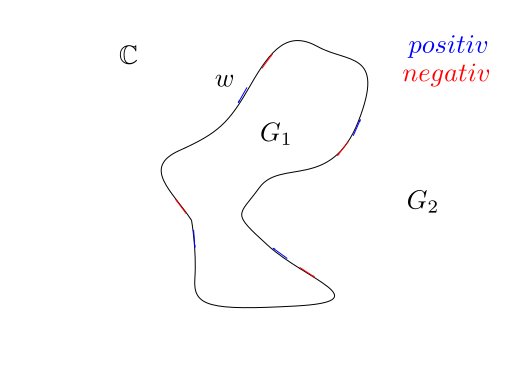
\includegraphics[width=\textwidth]{images/umlaufrichtung}
\caption{}
\end{figure}


\end{defi}

Ein wichtiges Integral:
Mit $m \in \mathbb{Z}$:

$$\oint_{|z-z_0|=r} (z-z_0)^{m} dz = 
\left\{  \begin{matrix}
0 & m \not= -1 \\
2 \pi i & m=-1
\end{matrix} \right.$$

%================================================================== Vorlesung 09.07.2013

\begin{figure}[H]
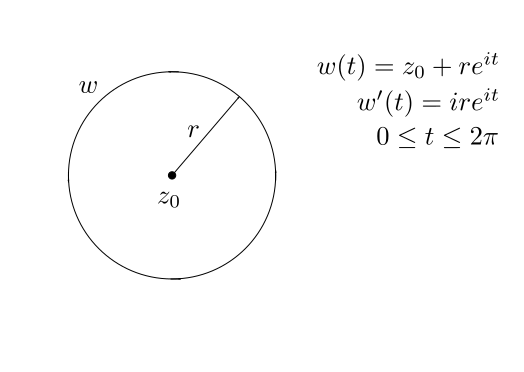
\includegraphics[width=\textwidth]{images/umlauf01}
\caption{Veranschaulichung des Integrals $\oint_{|z-z_0|=r} (z-z_0)^{m} dz$ und seiner Parametrisierung}
\end{figure}

$$\oint_{|z-z_0|=r} (z-z_0)^{m} dz = \int_{0}^{2\pi} \underbrace{(re^{it})^{m}}_{(w(t)-z_0)^{m}} \underbrace{ire^{it}}_{w'(t)} dt
= ir^{m+1} \int_{0}^{2\pi} e^{(m+1)it} dt$$

\begin{description}
\item[$m=-1$]: $$i \cdot 1 \cdot \int_{0}^{2\pi} 1 = 2\pi i $$
\item[$m \in \mathbb{Z}\backslash\{-1\}$]: $$ir^{m+1}  \left. \frac{e^{(m+1)it}}{(m+1)i}  \right|_{t=0}^{2 \pi} = ir^{(m+1)}(1-1)=0$$
\end{description}


\subsection{Der Integralsatz von Cauchy}

\begin{satz}[Integralsatz von Cauchy]
Sei $$f:U \rightarrow \mathbb{C} $$ komplex differenzierbar af dem offenen einfach zusammenhängenden Gebiet $U$ (d.h. keine "Löcher"). $w$ sei eine in $U$ verlaufenden einfach geschlossene Kurve (ohne Doppelpunkte). 

\begin{figure}[H]
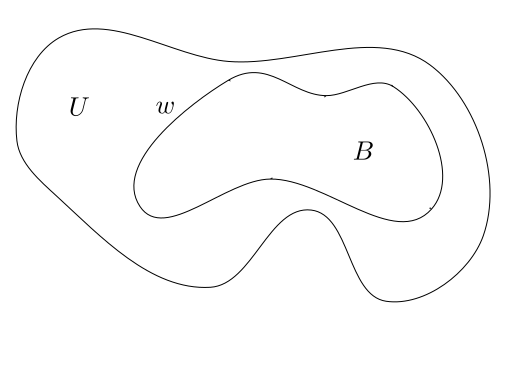
\includegraphics[width=\textwidth]{images/umlauf02}
% \caption{}
\end{figure}


Dann gilt

$$\int_{w} f(z) dz = 0$$

Zusatz: Dieser Satz gilt auch, wenn $w$ endlich viele Doppelpunkte hat.
\end{satz}

Nachweis mit dem Satz von Green für den Fall dass $f'$ stetig ist:
Ohne Einschränkung sei $w$ positiv orientiert. Das Innere heiße $B$.


\begin{eqnarray*}
Re\left(  \oint_{w} f(z) dz  \right) &=& \oint_{\tilde{w}=\partial \tilde{B}} \begin{pmatrix}
u \\ -v
\end{pmatrix} \cdot dx \\
& \stackrel{Green}{=}& \int_{\tilde{B}} \nabla^{T} \begin{pmatrix}
0 & 1 \\ -1 & 0
\end{pmatrix} \begin{pmatrix}
u \\-v
\end{pmatrix} df(x,y) \\
&=& \int_{\tilde{B}} \underbrace{(-v_x - u_y)}_{= 0 \text{ wegen CR-DGL}} dx dy \\
&=& 0
\end{eqnarray*}

\begin{eqnarray*}
Im\left(  \oint_{w} f(z) dz  \right) &=& \oint_{\tilde{w}=\partial \tilde{B}} \begin{pmatrix}
v \\ u
\end{pmatrix} \cdot dx  \\
&\stackrel{Green}{=}& \int_{\tilde{B}} \nabla^{T} \begin{pmatrix}
0 & 1 \\ -1 & 0
\end{pmatrix} \begin{pmatrix}
v \\u
\end{pmatrix} df(x,y) \\
&=& \int_{\tilde{B}} \underbrace{(u_x-v_y)}_{= 0 \text{ wegen CR-DGL}} dx dy \\
&=& 0
\end{eqnarray*}





$$\Rightarrow \oint_{w} f(z) dz =0$$

Bei endlich vielen Dopelpunkten: Zerlege die Schleife in einfach geschlossene Teilkurven

Bemerkung: Es ist zentral, dass $U$ einfach zusammenhängend ist. Denn dann ist $f$ holomorph auf dem inneren von $B$


\begin{bsp}[Cauchy auf nicht einfach zusammenhängendem Gebiet]

$$f(z)=\frac{1}{z}$$

$$U=\mathbb{C}\backslash \{0\}$$

Dann ist $f$ holomorph auf $U$, aber $U$ ist \emph{nicht} einfach zusammenhängend. Wir wissen $$\frac{1}{z}=(z-z_0)^{m} \text{ mit } m=-1, z_0=0$$

$$\oint_{|z|=0} \frac{1}{z} dz = 2 \pi i \not= 0$$
\end{bsp}



\begin{bsp}[Cachy-Integralsatz für $f(z)=z^{2}$]
$$U=\mathbb{C}$$

$$f(z)=z^{2}$$

$$m=2, z_0=0$$

Dann hatten wir berechnet: $\oint_{|z|=r} z^{2} dz = 0$ Das liefert auch der Cauchy-Integralsatz.
\end{bsp}

Folgerung: $f:U \rightarrow \mathbb{C}$ holomorph auf einfach zusammenhängendem, offenen Gebiet $U$. $w_1,w_2, \subset U$ verlaufen beiden von $z_0$ nach $z_1$ und $w_1 \cup w_2^{*}$ haben nur endlich viele Doppelpunkte. Dann $$\int_{w_1} f(z) d = \int_{w_2} f(z) dz$$

D.h. das Integral ist hier wegunabhängig.

Begründung: $$0=\int_{w_1 \cup w_2^{*}} f(z) dz = \int_{w_1} f(z) dz - \int_{w_2} f(z) dz$$

Wobei $w_2^{*}$ die gleiche Kurven wie $w_2$ ist, nur in entgegengesezte Richtung durchlaufen/parametrisiert.

\begin{figure}[H]
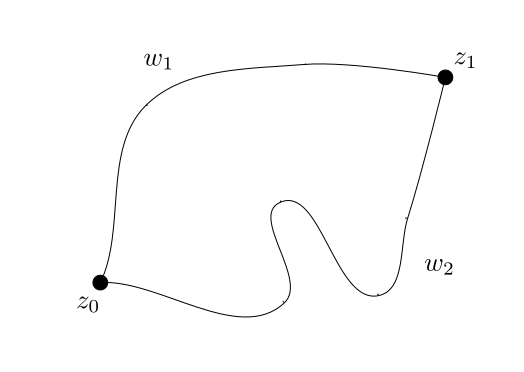
\includegraphics[width=\textwidth]{images/wegunabhangigkeit}
\caption{Skizze zum Nachweis bzw. Herleitung der komplexen Integration}
\end{figure}


Damit können wir komplexe Stammfunktionen berechnen.

\begin{satz}[Komplexe Integration]
$$U \subset \mathbb{C} $$ einfach zusammenhängend, offen $$f:U \rightarrow \mathbb{C}$$ holomorph auf $U$. Sei $z_0 \in U$ beliebig fest. Dann ist 
$$F(z) = \int_{z_0}^{z} f(z) dz = \int_{w} f(z) dz$$

mit $w$ eine beliebige Kurven in $U$ die $z_0$ mit $z$ verbindet.

\end{satz}

Nachweis:

\begin{figure}[H]
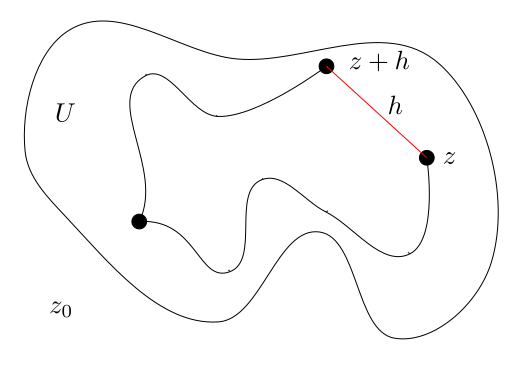
\includegraphics[width=\textwidth]{images/komplexe_integration}
\caption{Skizze zum Nachweis bzw. Herleitung der komplexen Integration}
\end{figure}



\begin{eqnarray*}
F(z+h)-F(z) &=& \int_{z_0}^{z+h} f(\xi) d\xi - \int_{z_0}^{z} f(\xi) d\xi \\
&=& \int_{z_0}^{z} f(\xi) d\xi + \int_{z}^{z+h} f(\xi) d\xi - \int_{z_0}^{z} f(\xi) d\xi \\
&=& \int_{z}^{z+h} f(\xi) d\xi = \int_{0}^{1} f(z+th) \cdot h ~ dt
\end{eqnarray*}



mit $$w(t)=z+ht,  0 \leq t \leq 1, w'(t)=h$$


$$\Rightarrow \frac{F(z+h)-F(z)}{h} = \int_{0}^{1} f(z+th) dt \stackrel{g \rightarrow 0}{\rightarrow} f(z) \Rightarrow F'(z)=f(z)$$

Berechnung von komplexen Integralen mit Hilfe der Stammfunktion:

\begin{satz}["Haupsatz" der komplexen Integralrechnung]
Ist $f$ analytisch auf $U \in \mathbb{C}$ und $F$ eine Stammfunktion von $f$ auf $U$, dann gilt für jede Kurve $w \subset U$:

$$\int_w f(z) dz = F(w(b))-F(w(a))$$

wobei $w:[a,b] \rightarrow \mathbb{C}$

Dies folgt aus $$\frac{d}{dt} F(w(t)) = F'(w(t))w'(t) = f(w(t))w'(t)$$

Also $$\int_{w} f(z) dz = \int_{a}^{b} f(w(t))w'(t) dt = \int_{a}^{b} \frac{d}{dt} F(w(t)) dt = F(w(b))-F(w(a))$$
\end{satz}

\subsection{Cauchy Integralformel}
Anmerkung:
Cauchy-Integralformel ist cooler, besser, schöner als der Cauchy Integralsatz!

\begin{satz}
$$U \subset \mathbb{C}$$ sei offen, aber eventuell nicht einfach zusammenhängend. Seien $w_1,w_2$ geschlossenen Kurven, die die Ausnahmemenge $A \subset \mathbb{C} \backslash U$ mit gleicher Orientierung umlaufen. Ist dann $f$ auf $U$ analytisch, dann gilt: $$\int_{w_1} f(z) dz = \int_{w_2} f(z) dz$$

\begin{figure}[H]
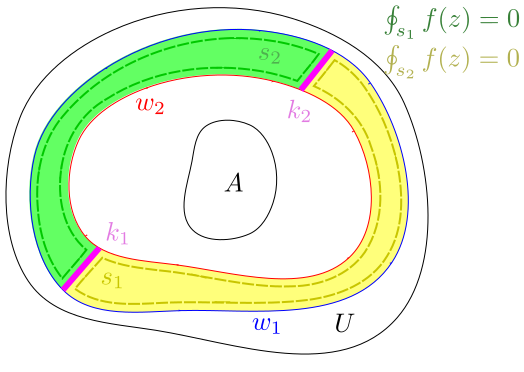
\includegraphics[width=\textwidth]{images/umlauf03}
\caption{Zwei gleichorientierte Kurven $w_1,w_2$ durchlaufen $U$ um das "Loch" $A$. Die zwei Kurven $w_1,w_2$ werden durch die "Schnitte" $k_1,k_2$ verbunden und es werden neue Kurven $s_1,s_2$ gebildet. Da sich die Linienintegrale $s_1,s_2$ auf den Schnitten gegenseitig aufheben (sie sind entgegengesetzt orientiert) entsprechen die Integrale von $s_1,s_2$ den Integralen von $w_1,w_2$. Der Vorteil von $s_1,s_2$ ist, dass diese nun auf einfach zusammenhängenden Gebieten liegen und wir sie daher einfach berechnen können.}
\end{figure}

Denn (Bild) 


\begin{eqnarray*}
0 &\stackrel{Cauchy Integrals.}{=}& \int_{s_1} f(z) dz + \int_{s_2} f(z) dz \\
&=& \int_{w_1} f(z) dz - \int_{w_2} f(z) dz \\
& & + \int_{k_1} f(z) dz - \int_{k_1} f(z) dz  \\
& & + \int_{k_2} f(z) dz - \int_{k_2} f(z) dz \\
&=& \int_{w_1} f(z) dz - \int_{w_2} f(z) dz
\end{eqnarray*}

\end{satz}

Speziell sei jetzt: $f:U \rightarrow \mathbb{C}, U \subset \mathbb{C} $ offen, $f$ analytisch. Sei $z \in U$ mit hinreichend kleinem $r$ gilt

$$K_r(z) = \{ \xi | |\xi - z| < r\} \subset U$$

\begin{figure}[H]
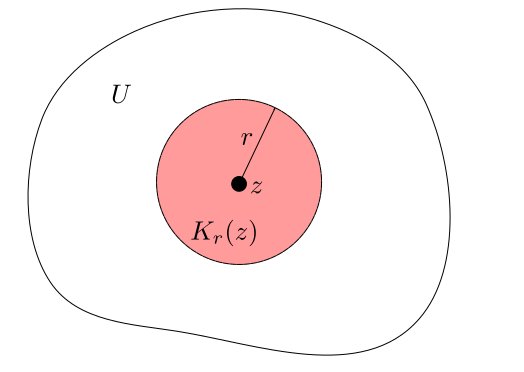
\includegraphics[width=\textwidth]{images/Kumz}
\caption{•}
\end{figure}

Die Funktion $$g(\xi) := \frac{f(\xi)}{\xi-z}$$ ist dann holomorph auf $K_r(z)\backslash\underbrace{\{z\}}_{=A}$. Nach obigem Satz gilt dann, dass alle Integrale $$\oint_{|\xi -z|=\rho} g(\xi) d\xi$$ für $0 < \rho < r$ den gleichen Integralwert $I$ haben.

Also: 

\begin{eqnarray*}
\forall 0 < \rho < r: \\
I &=& \oint_{|\xi-z|=\rho} \frac{f(\xi)}{\xi-z} d\xi \\
&=& \int_{0}^{2\pi} \frac{f(z+\rho e^{it})}{\rho e^{it}} i \rho e^{it} dt \\
&=& i \int_{0}^{2\pi} f(z+\rho e^{it}) dt \\
&\stackrel{\rho \rightarrow 0^{+}}{\rightarrow} & 2 \pi i f(z)
\end{eqnarray*}

wobei $w(t)=z+\rho e^{it} , 0\leq t \leq 2\pi, w'(t)=i\rho e^{it}$

dies führt zur wichtigen \emph{Cauchy Integralfomel}

\begin{defi}[Cauchy Integralfomel]
$$ \oint_{|\xi-z|=\rho} \frac{f(\xi)}{\xi-z} d \xi = 2 \pi i f(z)$$
$$ \forall 0 < \rho < r$$
\end{defi}

%========================================================================== Vorlesung 15.7.2013

\begin{satz}[Cauchy-Integralformel]
$$U \subset \mathbb{C}$$ ist ein offenes Gebiet. Und $$f: U \rightarrow \mathbb{C}$$
sei holomorph. $w$ sei eine einfach geschlossene Kruve in $U$, deren Inneres vollständig in $U$ liegt. Dann gilt für alle $z$ im Inneren von $B$
$$\oint_w \frac{f_\eta}{\eta-z} d\eta = 2 \pi i f(z)$$

Anmerkung: Wie sehen hier, dass die Kurve nicht unbedingt ein Kreis sein muss.
\end{satz}

Bemerkung: Insbesondere folgt daraus:

Ist $w$ die \emph{Randkruve} eine offenen Gebiets $W$ und $f$ holomorph in Umgebung von $\overline{W}$ ($\overline{W}=W \cup w$), dann ist $f$ auf $W$ vollstädnig durch die Werte auf $\partial W = w$ festgelegt.

\begin{bsp}[Berechnung eines Kruvenintegrals]

$$\oint_{|\zeta|=4} \frac{e^{\zeta}}{\zeta^{2}+3 \zeta} d\zeta$$

Mit Partialbruchzerlegung und Koeffizientenvergleich

\begin{eqnarray*}
\oint_{|\zeta|=4} \frac{e^{\zeta}}{\zeta^{2}+3 \zeta} d\zeta &=& \\
\oint_{|\zeta|=4} \frac{1}{3} \frac{e^{\zeta}}{\zeta} - \frac{1}{3} \frac{e^{\zeta}}{\zeta + 3} d\zeta &=& \\
\oint_{|\zeta|=4} \frac{1}{3} \frac{e^{\zeta}}{\zeta} d\zeta -  \oint_{|\zeta|=4} \frac{1}{3} \frac{e^{\zeta}}{\zeta + 3} d\zeta &=& \\
\text{mit Caucy Integralformel} \\
\underbrace{\frac{1}{3} 2\pi i e^{0}}_{z=0, f(\zeta)=e^{\zeta}} - \underbrace{\frac{1}{3} 2 \pi i e^{-3}}_{z=-3,f(\zeta)=e^{\zeta}} &=& \frac{2}{3} \pi i (1-e^{-3}) \\
\end{eqnarray*}
\end{bsp}


Weiter Folgerung aus Cauchy-Integralformel:

\begin{satz}[Ableiten der Cauchy-Integralformel]

$k$-faches Ableiten von $$f(z)=\frac{1}{2\pi i} \oint_w \frac{f(\zeta)}{\zeta - z} d\zeta$$ nach $z$ für alle $k \geq 0$

$$f^{(k)}(z) = \frac{k!}{2 \pi i} \oint_w \frac{f(\zeta)}{(\zeta - z)^{k+1}} d \zeta$$
\end{satz}

\subsection{Anwednungen der Cauchy-Integralformel}

\subsubsection{Taylor-Entwicklung}

Wir zeigen mit d. CIF (Cauchy-Integralformel): Ist $f$ in Umgebung von $z_0$ komplex differenzierbar, dann lässt sie sich in einer Kreisumgebung als Potenzreihe darstellen und ist daher $\infty$ oft komplex differenzierbar.

Wir verwenden eine Trick: Betrachte $z,z_0, \zeta \in \mathbb{C}$ mit $|z-z_0|<|\zeta-z_0|$

Dann 
\begin{eqnarray*}
\frac{1}{\zeta-z} &=& \frac{1}{(\zeta - z_0)-(z-z_0)} \\
&=& \frac{1}{\zeta - z_0} \cdot \frac{1}{1-\frac{z-z_0}{\zeta-z_0}} \\
&\stackrel{geom. Reihe}{=}& \frac{1}{\zeta-z_0} \sum_{k=0}^{\infty} \left( \frac{z-z_0}{\zeta-z_0} \right)^{k}
\end{eqnarray*}





Wir setzten in CIF ein: 
\begin{eqnarray*}
f(z)&=&\frac{1}{2 \pi i} \oint_w \frac{f(\zeta)}{\zeta-z} d\zeta \\
&=& \frac{1}{2 \pi i} \oint_w f(\zeta) \sum_{k=0}^{\infty} \frac{(z-z_0)^{k}}{(\zeta-z_0)^{k+1}} d\zeta \\
&=& \sum_{k=0}^{\infty} \underbrace{\left( \frac{1}{2 \pi i} \oint \frac{f(\zeta)}{(\zeta-z_0)^{k+1}} d\zeta \right)}_{a_k}(z-z_0)^{k}
\end{eqnarray*}




%=========================================================== Vorlesung 16.7.2013
\begin{satz}[Taylorreihe analytischer Funktionen]


$$f:U \rightarrow \mathbb{C}, U \subset \mathbb{C}$$

offenes Gebiet, $r >0 , z_0 \in U$ so, dass $K_R(z_0) \subset U$

Ist dann $0 < \rho < r$, dann ist $f(z)$ auf $K_\rho(z_0)$ als Potenzreihe (=Taylor-Reihe) darstellbar

$\forall t \in K_\rho(z_0)$:

$$f(z)=\sum_{k=0}^{\infty} a_k (z-z_0)^{k} = \sum_{k=0}^{\infty} \frac{f^{(k)}(z_0)}{k!}(z-z_0)^{k}$$ wobei

$$a_k=\frac{
1}{2 \pi i} \oint_{|\zeta-z_0|=\rho} \frac{f(\zeta)}{(\zeta-z_0)^{k+1}} d \zeta$$

Insbesondere ist $f$ in $z$ undendlich off differenzierbar.



\end{satz}

Bemerkung:
Taylor-Reihen sind eindeutig.

\begin{bsp}[Berechnung der Taylorreihe von $f(z)=\frac{1}{1+z}$ auf zwei Wegen]

Taylorreihe um $z_0=0$ via geometrischer Reihe.

$$|z| < 1 \Rightarrow \frac{1}{1+z}=\sum_{k=0}^{\infty} (-z)^{k} = \sum_{k=0}^{\infty} \underbrace{(-1)^{k}}_{a_k} z^{k}$$

Taylorriehe via $a_k=\frac{f^{(k)}(0)}{k!}$

$$f'(z)=-\frac{1}{(1+z)^{2}}$$
$$f''(z)=\frac{2}{(1+z)^{3}}$$
$$f'''(z)=-\frac{6}{(1+z)^{4}}$$
$$f^{(k)}(z)=-\frac{(-1)^{k} k!}{(1+z)^{k+1}}$$

$$\Rightarrow f^{(k)}(0) = (-1)^{k} k! \Rightarrow f(z)=\sum_{k=0}^{\infty} \frac{f^{(k)}(0)}{k!} z^{k} = \sum_{k=0}^{\infty} (-1)^{k} z^{k}$$
\end{bsp}


\subsubsection{Identitätssatz}


1. Vorgabe von allen Ableitungen in einem Punkt:


\begin{satz}
$$f:U \rightarrow \mathbb{C}, g:U \rightarrow \mathbb{C}$$
beide holomorph auf dem (zusammenhängenden) Gebiet und gebe es $z_0 \in U$ mit $f^{(k)}(z_0) = g^{(k)}(z_0) \; \forall k \geq 0$ dann gilt $$f(z)=g(z)$$ $\forall z \in U$ 
\end{satz}


2. Festlegung der Funktionswerte auf einer Kruve


\begin{satz}
$$f,g: U \rightarrow \mathbb{C}$$ sind holomorph auf dem (zusammenhängenden) Gebiet$U$ und ist $w \in U$ eine Kurve mit $w(a) \not= w(b)$, so dass $f(w(t))=g(w(t)), \forall t \in [a,b]$ dann gilt
$$f(z)=g(z), \forall z \in U$$
Folgerung: Stimmen holomorphe Funktionen auf $[a,b] \subset U (a < b)$ überein, so folgt $$f \equiv g$$
\end{satz}


\begin{bsp}


\begin{eqnarray*}
f(z)= f(x+iy) &=& [\underbrace{(x^{2}-y^{2})e^{3x}cos(3y)-2xye^{3x}sin(3y)}_{=u(x,y)}] \\
& & +i [\underbrace{2xye^{3x}cos(3y)+(x^{2}-y^{2})e^{3x}sin(3y)}_{=v(x,y)}]
\end{eqnarray*}


Behauptung: $f$ ist holomorph und es gitl $f(z)=z^{2}e^{3z}$


Begründung: Auswerten für $x \in  \mathbb{R}, y=0$ gibt jeweils $f(x)=x^{2}e^{3x}$



 Cauchy-Rieman-DGL prüfen $\Rightarrow$ holomorph $\Rightarrow$ Gleicheit, wegen Übereinstimmung auf $\mathbb{R}$

\end{bsp}

\subsubsection{Weiter Eigenschaften holomorpher Funktionen}

\begin{satz}
Ist $f$ auf $\mathbb{C}$ holomorph, dann ist $f$ entweder konstant oder unbeschränkt, d.h. $|f(z)| \leq M \forall z \in \mathbb{C} \Rightarrow f \equiv \text{ const auf } \mathbb{C}$ 

Begründung:

CIF: $|f'(z)| = \left|  \frac{1}{2 \pi i} \oint_{|\zeta -z|=\rho} \underbrace{\frac{f(\zeta)}{(\zeta-z)^{2}}}_{|\cdot| \leq \frac{M}{\rho^{2}}} d\zeta    \right| \leq \frac{1}{2 \pi} \underbrace{2 \pi \rho}_{\text{Kurvenlänge}} \frac{M}{\rho^{2}} = \frac{M}{\rho} \stackrel{\rho \rightarrow \infty}{\rightarrow} 0$



\end{satz}


\begin{satz}[Fundamentalsatz der Algebra]
Jedes nicht-konstate Polynom $p(z)$ besitzt auf $\mathbb{C}$ mindestens eine Nullstelle.

Nachweis: $p(z)= a_n z^{n} + \ldots  + a_1 z + a_0, n \geq 1, a_n \not= 0$

$|z|\rightarrow \infty \Rightarrow |p(z)| \rightarrow \infty$

Daher hat die stetige Funktion $z \longmapsto |p(z)|$ ein Minimum $z_m$ auf $\mathbb{C}$

Anmerkung:

$p(z) \not= 0 \forall z \in  \mathbb{C} \rightarrow |p(z_n)| = \gamma > 0$ Dann : $f(z)=\frac{1}{p(z)}$ ist holomorph. $|f(z)| \leq \frac{1}{\gamma} \forall z \in \mathbb{C}$

$\Rightarrow f$ beschränkt auf $\mathbb{C}$ (und holomorph) $\Rightarrow f \equiv const \Rightarrow p \equiv const$ Das ist aber ein Widerspruch.
\end{satz}


Weitere Eigenschaften

\begin{defi}[Mittelwerteigenschaft]
$$f$$ holomorph auf $K_r(z_0) , 0 < \rho < r \Rightarrow f(z_0) = \frac{1}{2 \pi} \int_{0}^{2\pi} f(z_0+ \rho e^{it}) dt$
\end{defi}

\begin{defi}[Maximumsprinzip]
$$f: U \rightarrow \mathbb{C}$$ holomorph und nicht konstant auf dem offenen Gebiet $U \subset \mathbb{C}$ dann hat $|f|$ auf $U$ kein Maximum.
 \end{defi}

\subsection{Laurentreihen}
Laurentreihen "leben" auf Kreisringen $$K_{r,R}(z) = \{ z | r < |z-z_0|<R\}$$ 
auf denen $f$ holomorph ist. $\overline{K_r(z_0)}$ darf Punkte enthalten, in denen $f$ nicht holomorph ist.

\begin{defi}[Laurent-Reihe von $f$]

$$f(z)=\sum_{k=- \infty}^{\infty} c_k (z-z_0)^{k} = \underbrace{\sum_{k=1}^{\infty} c_{-k} (z-z_0)^{k}}_{\text{Hauptteil}} + \underbrace{\sum_{k=0}^{\infty} c_k (z-z_0)^{k}}_{\text{Nebenteil}}$$

\end{defi}


\begin{satz}[Larent-Entwicklung auf Kreisring]

\begin{figure}[H]
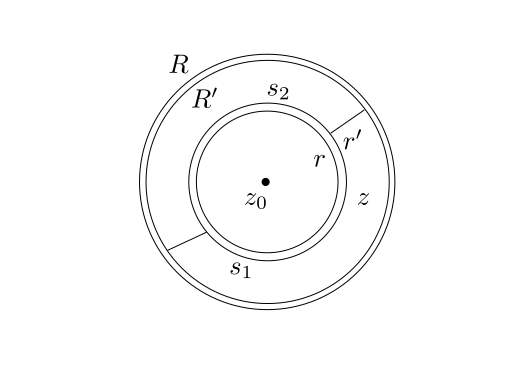
\includegraphics[width=\textwidth]{images/laurent}
\caption{•}
\end{figure}

$$f$$ sei holomorph auf $K_{r,R}(z_0), 0 \leq r < R \leq \infty$ dann kann $f$ auf $K_{r,R}(z_0)$ als \emph{Laurent-Reihe} geschrieben werden 
$$f(z)=\sum_{k=-\infty}^{\infty} c_k (z-z_0)^{k}, \forall z \in K_{r,R}(z_0)$$ Wobei


$$c_k = \frac{1}{2 \pi i } \oint_{|\zeta-z_0|=\rho} \frac{\zeta}{\zeta-z_0}^{k+1} d\zeta , \forall k \in \mathbb{Z}, r < \rho < R$$

Der Hauptteil konvergiert absolut und gleichmäßig auf $K_{r',\infty}(z_0)$ für $r' > r$
Der Nebenteil konvergiert absolut und gleichmäßig auf $K_{R'}(z_0)$ für $R'<R$
\end{satz}

Herleitung der Laurentreihe: Wähle $0<r<r'<R'<R$

Integrand $\frac{f(\zeta)}{\zeta-z}$

mit $z \in K_{r',R'}(z_0)$

CIF: $f(z) = \frac{1}{2 \pi i} \oint_{s_1} \frac{f(\zeta)}{\zeta-z} d\zeta$
$0 = \frac{1}{2 \pi i} \oint_{s_2} \frac{f(\zeta)}{\zeta-z} d\zeta$

Zusammen

\begin{eqnarray*}
f(z) &=& \frac{1}{2 \pi i} \oint_{s_1} \frac{f(\zeta)}{\zeta-z} d\zeta + \frac{1}{2 \pi i} \oint_{s_2} \frac{f(\zeta)}{\zeta-z} d\zeta = \\
 &=& \frac{1}{2 \pi i} \oint_{|\zeta - z_0| = R'} \frac{f(\zeta)}{\zeta-z} d\zeta + \frac{1}{2 \pi i} \oint_{|\zeta - z_0|=r'} \frac{f(\zeta)}{\zeta-z} d\zeta =
\end{eqnarray*}

Für $|\zeta-z|=R' > |z-z_0|$

$\stackrel{Taylor}{\Rightarrow} \frac{1}{\zeta-z} =  \ldots = \sum_{k=0}^{\infty} \frac{(z-z_0)^{k}}{(\zeta-z_0)^{k+1}}$

Für $|\zeta-z_0|=r'$
$\frac{1}{\zeta-z_0}=\frac{-1}{z-z_0} \frac{1}{1-\frac{\zeta-z_0}{z-z_0}} \stackrel{geom. Reihe}{=} - \frac{1}{z-z_0} \sum_{k=0}^{\infty} \left( \frac{\zeta - z_0}{z-z_0}\right)^{k}$
\newpage

\section{Indices}

\subsection{Liste aller Definitionen}
\listtheorems{defi}

\subsection{Liste aller Sätze}
\listtheorems{satz}

\subsection{Liste aller Beispiele}
\listtheorems{bsp}


\end{document}
